\setcounter{dang}{0}
\setcounter{ex}{0}
\section{Mức độ 7,8,9,10}
\Opensolutionfile{ans}[ans/CD7/DA2]
\begin{dang}
	{Góc giữa đường thẳng với đường thẳng}
\end{dang}
\begin{ex}%[1H3B2-3]
	[Mã 101 - 2021 Lần 1]
    \immini{Cho hình lăng trụ đứng $ABC.A'B'C'$ có tất cả các cạnh bằng Góc giữa đường thẳng $AA'$ và $BC'$ bằng
        \choice
        {$30^{\circ}$}
        {$90^{\circ}$}
        {\True $45^{\circ}$}
        {$60^{\circ}$}}
    {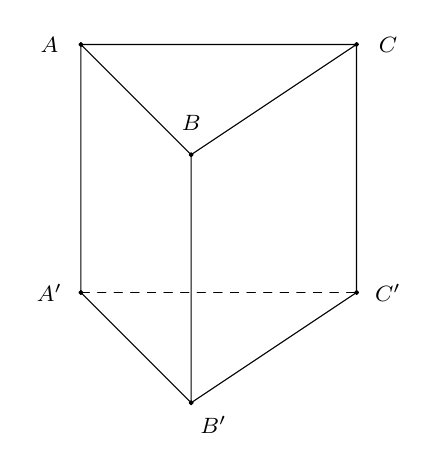
\begin{tikzpicture}[scale=0.7, font=\footnotesize, line join=round, line cap=round, >=stealth]
            \path
            (0,0) coordinate (A)
            (2,-2) coordinate (B)
            (5,0) coordinate (C) ;
            \foreach \x in {A,B,C}
            \path (\x)+(0,-4.5) coordinate(\x');
            \draw[dashed] (A')--(C');
            \draw(A')--(B')--(C') (A')--(A)--(B)--(C)--(C') (B)--(B') (A)--(C);
            \foreach \p/\g in {A/180,B/90,C/0,A'/180,B'/-45,C'/0}\draw[fill=black] (\p) circle (1pt)node[shift={(\g:.4)}]{$\p$};
    \end{tikzpicture}}
    \loigiai{
        \immini{Vì $AA'\parallel BB'$ nên $(AA',BC')=(BB',BC')=\widehat{B'BC}$.\\
            Ta có $\tan\widehat{B'BC}=\dfrac{B'C'}{BB'}=1\Rightarrow\widehat{B'BC}=45^{\circ}$.}
        {\begin{tikzpicture}[scale=0.7, font=\footnotesize, line join=round, line cap=round, >=stealth]
                \path
                (0,0) coordinate (A)
                (2,-2) coordinate (B)
                (5,0) coordinate (C) ;
                \foreach \x in {A,B,C}
                \path (\x)+(0,-4.5) coordinate(\x');
                \draw[dashed] (A')--(C');
                \draw(A')--(B')--(C') (A')--(A)--(B)--(C)--(C')--(B)--(B') (A)--(C);

                \foreach \p/\g in {A/180,B/90,C/0,A'/180,B'/-45,C'/0}\draw[fill=black] (\p) circle (1pt)node[shift={(\g:.4)}]{$\p$};
                \pic[draw,angle radius=3.5mm,angle eccentricity=1.5] {angle = B'--B--C'};
        \end{tikzpicture}}
    }
\end{ex}

\begin{ex}%[Mã 103 - 2021 - Lần 1]%Câu 2.%[1H3B2-3]
    \immini{Cho hình lăng trụ đứng $ABC.A'B'C'$ có tất cả các cạnh bằng nhau (tham khảo hình bên dưới).
        Góc giữa hai đường thẳng $A'B$ và $CC'$ bằng
        \choice
        {\True $45^{\circ}$}
        {$30^{\circ}$}
        {$90^{\circ}$}
        {$60^{\circ}$}}
    {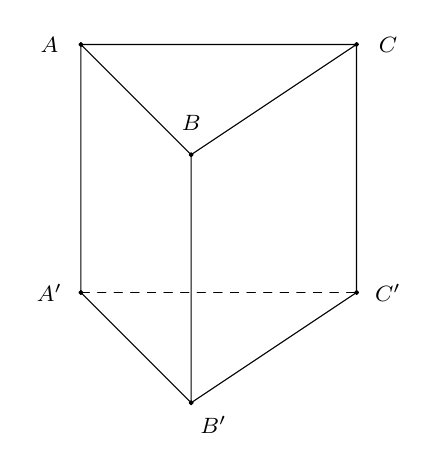
\begin{tikzpicture}[scale=0.7, font=\footnotesize, line join=round, line cap=round, >=stealth]
            \path
            (0,0) coordinate (A)
            (2,-2) coordinate (B)
            (5,0) coordinate (C) ;
            \foreach \x in {A,B,C}
            \path (\x)+(0,-4.5) coordinate(\x');
            \draw[dashed] (A')--(C');
            \draw(A')--(B')--(C') (A')--(A)--(B)--(C)--(C') (B)--(B') (A)--(C);
            \foreach \p/\g in {A/180,B/90,C/0,A'/180,B'/-45,C'/0}\draw[fill=black] (\p) circle (1pt)node[shift={(\g:.4)}]{$\p$};
    \end{tikzpicture}}
    \loigiai{
        \immini{Ta có $CC'\parallel BB'$. Nên $\left(\widehat{A'B; CC'}\right) =\left(\widehat{A'B; BB'}\right)$ = $\widehat{A'BB'}$ ( $\widehat{A'BB'}$ là góc nhọn).\\
            Mặt khác, tam giác $A'BB'$ là tam giác vuông cân ($A'B=BB'$ và $A'B\perp BB'$) suy ra $\widehat{A'BB'}=45^{\circ}$.\\
            Vậy góc giữa hai đường thẳng $A'B$ và $CC'$ bằng $45^{\circ}$.}
        {\begin{tikzpicture}[scale=0.7, font=\footnotesize, line join=round, line cap=round, >=stealth]
                \path
                (0,0) coordinate (A)
                (2,-2) coordinate (B)
                (5,0) coordinate (C) ;
                \foreach \x in {A,B,C}
                \path (\x)+(0,-4.5) coordinate(\x');
                \draw[dashed] (A')--(C');
                \draw(A')--(B')--(C') (B)--(A')--(A)--(B)--(C)--(C') (B)--(B') (A)--(C);
                \foreach \p/\g in {A/180,B/90,C/0,A'/180,B'/-45,C'/0}\draw[fill=black] (\p) circle (1pt)node[shift={(\g:.4)}]{$\p$};
                \pic[draw,angle radius=3.5mm,angle eccentricity=1.5] {angle = A'--B--B'};
        \end{tikzpicture}}
    }
\end{ex}

\begin{ex}%[Mã 102 - 2021 Lần 1]%Câu 3.%[1H3B2-3]
    \immini{Cho hình lăng trụ đứng $ABC.A'B'C'$ có tất cả các cạnh bằng nhau (tham khảo hình bên).
        Góc giữa hai đường thẳng $AA'$ và $B'C$ bằng
        \choice
        {$90^{\circ}$}
        {\True $45^{\circ}$}
        {$30^{\circ}$}
        {$60^{\circ}$}}
    {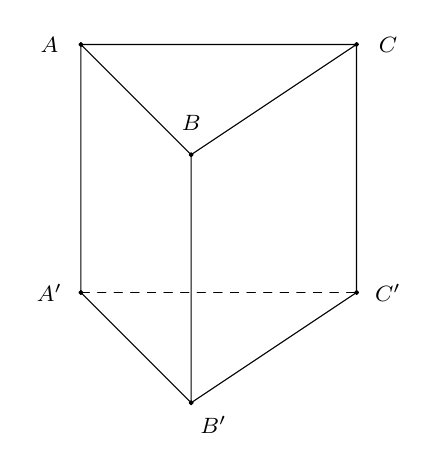
\begin{tikzpicture}[scale=0.7, font=\footnotesize, line join=round, line cap=round, >=stealth]
            \path
            (0,0) coordinate (A)
            (2,-2) coordinate (B)
            (5,0) coordinate (C) ;
            \foreach \x in {A,B,C}
            \path (\x)+(0,-4.5) coordinate(\x');
            \draw[dashed] (A')--(C');
            \draw(A')--(B')--(C') (A')--(A)--(B)--(C)--(C') (B)--(B') (A)--(C);
            \foreach \p/\g in {A/180,B/90,C/0,A'/180,B'/-45,C'/0}\draw[fill=black] (\p) circle (1pt)node[shift={(\g:.4)}]{$\p$};
    \end{tikzpicture}}
    \loigiai{
        \immini{Ta có $AA'\parallel CC'$ nên
            $(AA',B'C)=(CC',B'C)$.\\
            Mặt khác tam giác $BCC'$ vuông tại $C'$ có $CC'=B'C'$ nên là tam giác vuông cân.\\
            Vậy góc giữa hai đường thẳng $AA'$ và $B'C$ bằng $45^{\circ}$.}
        {\begin{tikzpicture}[scale=0.7, font=\footnotesize, line join=round, line cap=round, >=stealth]
                \path
                (0,0) coordinate (A)
                (2,-2) coordinate (B)
                (5,0) coordinate (C) ;
                \foreach \x in {A,B,C}
                \path (\x)+(0,-4.5) coordinate(\x');
                \draw[dashed] (A')--(C');
                \draw(A')--(B')--(C') (A')--(A)--(B)--(C)--(C') (B)--(B')--(C) (A)--(C);
                \foreach \p/\g in {A/180,B/90,C/0,A'/180,B'/-45,C'/0}\draw[fill=black] (\p) circle (1pt)node[shift={(\g:.4)}]{$\p$};
                \pic[draw,angle radius=3.5mm,angle eccentricity=1.5] {angle = B'--C--C'};
        \end{tikzpicture}}
    }
\end{ex}

\begin{ex}%[Mã 104 - 2021 Lần 1]%Câu 4.%[1H3B2-3]
    \immini{Cho hình lăng trụ đứng $ABC.A'B'C'$ có tất cả các cạnh bằng nhau (tham khảo hình bên).
        Góc giữa hai đường thẳng $AB'$ và $CC'$ bằng
        \choice
        {$30^{\circ}$}
        {$90^{\circ}$}
        {$60^{\circ}$}
        {\True $45^{\circ}$}}
    {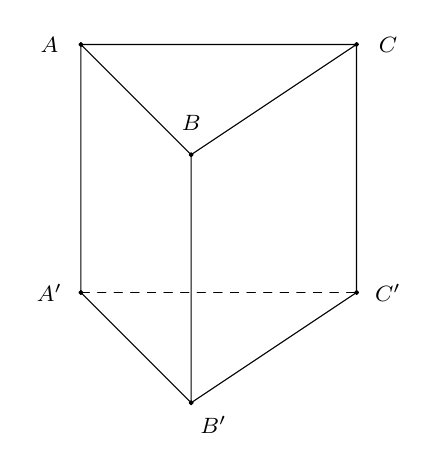
\begin{tikzpicture}[scale=0.7, font=\footnotesize, line join=round, line cap=round, >=stealth]
            \path
            (0,0) coordinate (A)
            (2,-2) coordinate (B)
            (5,0) coordinate (C) ;
            \foreach \x in {A,B,C}
            \path (\x)+(0,-4.5) coordinate(\x');
            \draw[dashed] (A')--(C');
            \draw(A')--(B')--(C') (A')--(A)--(B)--(C)--(C') (B)--(B') (A)--(C);
            \foreach \p/\g in {A/180,B/90,C/0,A'/180,B'/-45,C'/0}\draw[fill=black] (\p) circle (1pt)node[shift={(\g:.4)}]{$\p$};
    \end{tikzpicture}}
    \loigiai{
        \immini{Ta có $BB'\parallel CC'$ (do $BB'$ và $CC'$ là cạnh bên của hình lăng trụ).\\
            Suy ra $\left(\widehat{AB',CC'}\right)=\left(\widehat{AB',BB'}\right)$.\\
            Tứ giác $ABB'A'$ là hình vuông (do $ABC.A'B'C'$ là lăng trụ đứng có tất cả các cạnh bằng nhau) nên $\widehat{AB'B}=45^{\circ}$.\\
            Vậy $\left(\widehat{AB',CC'}\right)=\left(\widehat{AB',BB'}\right)=\widehat{AB'B}=45^{\circ}$.}
        {\begin{tikzpicture}[scale=0.7, font=\footnotesize, line join=round, line cap=round, >=stealth]
                \path
                (0,0) coordinate (A)
                (2,-2) coordinate (B)
                (5,0) coordinate (C) ;
                \foreach \x in {A,B,C}
                \path (\x)+(0,-4.5) coordinate(\x');
                \draw[dashed] (A')--(C');
                \draw(A')--(B')--(C') (A')--(A)--(B)--(C)--(C') (B)--(B')--(A)--(C);
                \foreach \p/\g in {A/180,B/90,C/0,A'/180,B'/-45,C'/0}\draw[fill=black] (\p) circle (1pt)node[shift={(\g:.4)}]{$\p$};
                \pic[draw,angle radius=3.5mm,angle eccentricity=1.5] {angle = B--B'--A};
        \end{tikzpicture}}
    }
\end{ex}

\begin{ex}%[Đề Tham Khảo 2018]%Câu 5.%[1H3B2-3]
    \immini{Cho tứ diện $OABC$ có $OA$, $OB$, $OC$ đôi một vuông góc với nhau và $OA=OB=OC$. Gọi $M$ là trung điểm của $BC$ (tham khảo hình vẽ bên dưới). Góc giữa hai đường thẳng $OM$ và $AB$ bằng
        \choice
        {$45^{\circ}$}
        {$90^{\circ}$}
        {$30^{\circ}$}
        {\True $60^{\circ}$}}
    {\begin{tikzpicture}[>=stealth,line join=round,line cap=round,font=\footnotesize,scale=0.8]
            \path (0,0) coordinate (O)
            (3,-2.5) coordinate (C)
            (6,0) coordinate (B)
            ($(O)+(0,4)$)coordinate (A)
            ($(B)!0.5!(C)$)coordinate (M)
            ;
            \draw (C)--(O)--(A)--(B)--(C)--(A);
            \draw[dashed] (M)--(O)--(B);
            \foreach \p / \r in {A/90,B/0,C/-90,O/180,M/-45}
            \fill (\p) circle (1.2pt) node[shift={(\r:3mm)}]{$\p$};
    \end{tikzpicture}}
    \loigiai{
        \immini{Đặt $OA=a$ suy ra $OB=OC=a$ và $AB=BC=AC=a\sqrt{2}$.\\
            Gọi $N$ là trung điểm $AC$ ta có $MN\parallel AB$ và $MN=\dfrac{a\sqrt{2}}{2}$.\\
            Suy ra góc $\widehat{(OM,AB)}=\widehat{(OM,MN)}$. Xét $\widehat{OMN}$.\\
            Trong tam giác $OMN$ có $ON=OM=MN=\dfrac{a\sqrt{2}}{2}$ nên $OMN$ là tam giác đều.\\
            Suy ra $\widehat{OMN}=60^{\circ}$.\\
            Vậy $\widehat{(OM,AB)}=\widehat{(OM,MN)}=60^{\circ}$.}
        {\begin{tikzpicture}[>=stealth,line join=round,line cap=round,font=\footnotesize,scale=0.8]
                \path (0,0) coordinate (O)
                (3,-2.5) coordinate (C)
                (6,0) coordinate (B)
                ($(O)+(0,4)$)coordinate (A)
                ($(B)!0.5!(C)$)coordinate (M)
                ($(A)!0.5!(C)$)coordinate (N)
                ;
                \draw (C)--(O)--(A)--(B)--(C)--(A) (O)--(N)--(M);
                \draw[dashed] (M)--(O)--(B);
                \foreach \p / \r in {A/90,B/0,C/-90,O/180,M/-45,N/70}
                \fill (\p) circle (1.2pt) node[shift={(\r:3mm)}]{$\p$};
        \end{tikzpicture}}
    }
\end{ex}

\begin{ex}%[Chuyên Long An - 2021]%Câu 6.%[1H3B2-3]
    Cho hình lập phương $ABCD.EFGH$. Góc giữa cặp véc-tơ $\overrightarrow{AF}$ và $\overrightarrow{EG}$ bằng
    \choice
    {$30^{\circ}$}
    {$120^{\circ}$}
    {\True $60^{\circ}$}
    {$90^{\circ}$}
    \loigiai{
        \immini{Ta có $\left(\overrightarrow{AF},\overrightarrow{EG}\right)=\left(\overrightarrow{AF},\overrightarrow{AC}\right)=\widehat{CAF}$.\\
            $\triangle CAF$ là tam giác đều, nên $\widehat{CAF}=60^{\circ}$.}
        {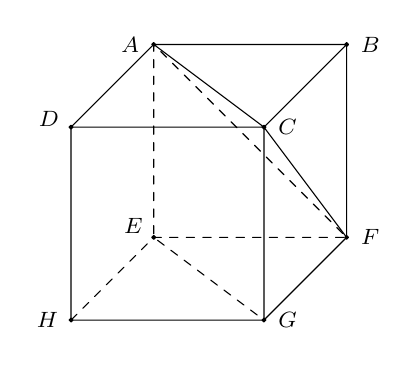
\begin{tikzpicture}[scale=.7, font=\footnotesize, line join=round, line cap=round, >=stealth]
                \path
                (0,0) coordinate (D)
                (3.5,0) coordinate (C)
                (1.5,1.5) coordinate (A)
                (A)+(C) coordinate (B);
                \path (A)+(0,-3.5) coordinate(E);
                \path (B)+(0,-3.5) coordinate(F);
                \path (C)+(0,-3.5) coordinate(G);
                \path (D)+(0,-3.5) coordinate(H);
                \draw[dashed] (H)--(E)--(F)--(A)--(E)--(G);
                \draw (B)--(F)--(G)  (A)--(D)--(C)--(A)--(B)--(C)--(G) (C)--(F) (D)--(H)--(G);
                \foreach \p/\g in {E/150,F/0,G/0,H/180,A/180,B/0,C/0,D/160}\draw[fill=black] (\p) circle (1pt)node[shift={(\g:.3)}]{$\p$};
        \end{tikzpicture}}
    }
\end{ex}

\begin{ex}%[THPT Nguyễn Huệ - Phú Yên - 2021]%Câu 7.%[1H3K2-2]
    Hình chóp $S.ABC$ có $SA$, $SB$, $SC$ đôi một vuông góc với nhau và $SA=SB=SC$. Gọi $I$ là trung điểm của $AB$. Góc giữa $SI$ và $BC$ bằng
    \choice
    {$30^{\circ}$}
    {\True $60^{\circ}$}
    {$45^{\circ}$}
    {$90^{\circ}$}
    \loigiai{
        \immini{Ta có
            \begin{eqnarray*}
                \cos\left(\overrightarrow{SI};\overrightarrow{BC}\right)&=& \dfrac{\overrightarrow{SI}\cdot\overrightarrow{BC}}{SI\cdot BC}=\dfrac{\dfrac{1}{2}\left(\overrightarrow{SA}+\overrightarrow{SB}\right)\cdot\overrightarrow{BC}}{\dfrac{BC}{2}\cdot BC}\\
                &= & \dfrac{\overrightarrow{SA}\cdot\overrightarrow{BC}+\overrightarrow{SB}\cdot\overrightarrow{BC}}{BC^2}=\dfrac{\overrightarrow{SB}\cdot\overrightarrow{BC}}{BC^2}\\
                &= &\dfrac{SB\cdot BC\cdot\cos 135^{\circ}}{BC^2}=\dfrac{SB\cdot SB\sqrt{2}\cdot\cos 135^{\circ}}{2SB^2}\\
                &= & \dfrac{\sqrt{2}\cdot\cos 135^{\circ}}{2}=-\dfrac{1}{2}.
            \end{eqnarray*}
            Suy ra $\left(\overrightarrow{SI};\overrightarrow{BC}\right)=120^{\circ}\Rightarrow(SI;BC)=60^{\circ}$.}
        {\begin{tikzpicture}[>=stealth,line join=round,line cap=round,font=\footnotesize,scale=0.8]
                \path (0,0) coordinate (S)
                (3,-2.5) coordinate (C)
                (6,0) coordinate (B)
                ($(S)+(0,4)$)coordinate (A)
                ($(B)!0.5!(A)$)coordinate (I)
                ;
                \draw (C)--(S)--(A)--(B)--(C)--(A);
                \draw[dashed] (I)--(S)--(B);
                \foreach \p / \r in {A/90,B/0,C/-90,S/180,I/45}
                \fill (\p) circle (1.2pt) node[shift={(\r:3mm)}]{$\p$};
        \end{tikzpicture}}
    }
\end{ex}

\begin{ex}%[THPT Nguyễn Đức Cảnh - Thái Bình - 2021]%Câu 8.%[1H3B2-3]
    Cho hình lập phương $ABCD.A_1B_1C_1D_1$ có cạnh $a$. Gọi $I$ là trung điểm $BD$. Góc giữa hai đường thẳng $A_1D$ và $B_1I$ bằng
    \choice
    {$120^{\circ}$}
    {\True $30^{\circ}$}
    {$45^{\circ}$}
    {$60^{\circ}$}
    \loigiai{
        \immini{Ta có $B_1C\parallel A_1D\Rightarrow(A_1D, B_1I)=(B_1C, B_1I)$.\\
            Vì $ABCD.A_1B_1C_1D_1$ là hình lập phương cạnh $a$ nên $B_1C=a\sqrt{2}; IC=\dfrac{a\sqrt{2}}{2}; B_1I=\dfrac{a\sqrt{6}}{2}$.\\
            Xét $\triangle B_1IC$ có $\cos\widehat{IB_1C}=\dfrac{B_1I^2+B_1C^2-IC^2}{2B_1I\cdot B_1C}=\dfrac{\sqrt{3}}{2}$ \\
            $ \Rightarrow\widehat{IB_1C}=30^{\circ} $.\\
            Do đó $\left(A_1D, B_1I\right)=(B_1C, B_1I)=\widehat{IB_1C}=30^{\circ}$.}
        {\begin{tikzpicture}[scale=0.7, font=\footnotesize, line join=round, line cap=round, >=stealth]
                \path
                (0,0) coordinate (A)
                (3.5,0) coordinate (B)
                (1.5,1.5) coordinate (D)
                (D)+(B) coordinate (C)
                ($(B)!0.5!(D)$) coordinate (I)
                ;
                \path (A)+(0,3.5) coordinate(A_1);
                \path (B)+(0,3.5) coordinate(B_1);
                \path (C)+(0,3.5) coordinate(C_1);
                \path (D)+(0,3.5) coordinate(D_1);
                \draw[dashed] (C)--(A)--(D)--(C) (A_1)--(D)--(D_1) (C)--(I)--(B_1);
                \draw (A_1)--(A)--(B)--(C)--(C_1)--(D_1)--(A_1)--(B_1)--(B) (B_1)--(C_1) (B_1)--(C);
                \foreach \p/\g in {A/-90,B/-90,C/0,D/180,A_1/180,B_1/0,C_1/0,D_1/160,I/-110}\draw[fill=black] (\p) circle (1pt)node[shift={(\g:.4)}]{$\p$};
        \end{tikzpicture}}
    }
\end{ex}

\begin{ex}%[THPT Lê Quý Đôn Điện Biên 2019]%Câu 9.%[1H3K2-2]
    Cho tứ diện $ABCD$ với $AC=\dfrac{3}{2}AD$, $\widehat{CAB}=\widehat{DAB}=60^{\circ}$, $CD=AD$. Gọi $\varphi$ là góc giữa hai đường thẳng $AB$ và $CD$. Chọn khẳng định đúng về góc $\varphi$.
    \choice
    {$\cos\varphi=\dfrac{3}{4}$}
    {$30^{\circ}$}
    {$60^{\circ}$}
    {\True $\cos\varphi=\dfrac{1}{4}$}
    \loigiai{
        \immini{Ta có
            \begin{eqnarray*}
                \overrightarrow{AB}\cdot\overrightarrow{CD}&=& \overrightarrow{AB}\cdot\left(\overrightarrow{AD}-\overrightarrow{AC}\right)=\overrightarrow{AB}\cdot\overrightarrow{AD}-\overrightarrow{AB\cdot}\overrightarrow{AC}\\
                &= & AB\cdot AD\cdot \cos 60^{\circ}-AB\cdot AC\cdot \cos 60^{\circ}\\
                &= & AB\cdot AD\cdot \cos 60^{\circ}-AB\cdot\dfrac{3}{2}AD\cdot \cos 60^{\circ}\\
                &= &\dfrac{-1}{4}AB\cdot AD.
            \end{eqnarray*}
            $\cos\left(\overrightarrow{AB},\overrightarrow{CD}\right)=\dfrac{\overrightarrow{AB}\cdot\overrightarrow{CD}}{AB\cdot CD}=\dfrac{-1}{4}\Rightarrow \cos\varphi=\dfrac{1}{4}$.}
        {\begin{tikzpicture}[font=\footnotesize, line join=round, line cap=round, >=stealth]
                \path 	(0:0) coordinate (B)
                ++(0:4) coordinate (D)
                ++(-145:3) coordinate (C)
                ($(B)+(60:3)$) coordinate (A);
                \draw 	(A)--(C)--(B)--(A)--(D)--(C);
                \draw[dashed] 	(D)--(B);
                \draw pic[draw,angle radius=17,angle eccentricity=1.5]{angle=B--A--C};
                \draw pic[draw,angle radius=15,angle eccentricity=1.5]{angle=B--A--D};
                \draw (1.3,2)node[below]{$60^\circ$};
                \draw (1.9,2.1)node[below]{$60^\circ$};
                \foreach \x /\goc in {A/90,B/180,C/-90,D/0}
                \fill[black] (\x) circle (1pt)
                ($(\x)+(\goc:3mm)$) node {$\x$};
        \end{tikzpicture}}
    }
\end{ex}

\begin{ex}%[THPT Hoàng Hoa Thám Hưng Yên 2019]%Câu 10.%[1H3B2-3]
    \immini{Cho hình hộp chữ nhật $ABCD.A'B'C'D'$, biết đáy $ABCD$ là hình vuông. Tính góc giữa $A'C$ và $BD$.
        \choice
        {\True $90^{\circ}$}
        {$30^{\circ}$}
        {$60^{\circ}$}
        {$45^{\circ}$}}
    {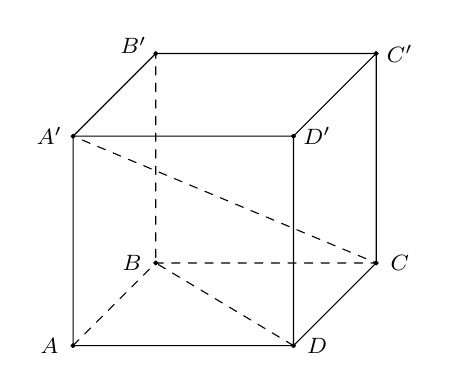
\begin{tikzpicture}[scale=0.7, font=\footnotesize, line join=round, line cap=round, >=stealth]
            \path
            (0,0) coordinate (A)
            (4,0) coordinate (D)
            (1.5,1.5) coordinate (B)
            (B)+(4,0) coordinate (C);
            \foreach \x in {A,B,C,D}
            \path (\x)+(0,3.8) coordinate(\x');
            \draw[dashed] (A)--(B)--(C)--(A') (D)--(B)--(B');
            \draw(A')--(D')--(C')--(B')--(A')--(A)--(D)--(C)--(C') (D)--(D');
            \foreach \p/\g in {A/180,D/0,C/0,B/180,A'/180,D'/0,C'/0,B'/160}\draw[fill=black] (\p) circle (1pt)node[shift={(\g:.3)}]{$\p$};
    \end{tikzpicture}}
    \loigiai{
        Vì $ABCD$ là hình vuông nên $BD\perp AC$.\\
        Mặt khác $AA'\perp(ABCD)\Rightarrow BD\perp AA'$.\\
        Ta có $\heva{& BD\perp AC\\& BD\perp AA'}\Rightarrow BD\perp(AA'C)\Rightarrow BD\perp A'C$.\\
        Do đó góc giữa $A'C$ và $BD$ bằng $90^{\circ}$.
    }
\end{ex}

\begin{ex}%[Chuyên KHTN 2019]%Câu 11.%[1H3B2-3]
    Cho tứ diện $ABCD$ có $AB=CD=2a$. Gọi $M$, $N$ lần lượt là trung điểm $AD$ và $BC$. Biết $MN=a\sqrt{3}$, góc giữa hai đường thẳng $AB$ và $CD$ bằng
    \choice
    {$45^{\circ}$}
    {$90^{\circ}$}
    {\True $60^{\circ}$}
    {$30^{\circ}$}
    \loigiai{
        \immini{Gọi $P$ là trung điểm $AC$, ta có $PM\parallel CD$ và $PN\parallel AB$, suy ra $\left(\widehat{AB,CD}\right)=\left(\widehat{PM,PN}\right)$.\\
            Dễ thấy $PM=PN=a$.\\
            Xét $\triangle PMN$ ta có
            \begin{eqnarray*}
                \cos\widehat{MPN}&= & \dfrac{PM^2+PN^2-MN^2}{2PM\cdot PN}\\
                &= & \dfrac{a^2+a^2-3a^2}{2\cdot a\cdot a}=-\dfrac{1}{2}\\
            \end{eqnarray*}
            $ \Rightarrow\widehat{MPN}=120^{\circ}\Rightarrow\left(\widehat{AB,CD}\right)=180^{\circ}-120^{\circ}=60^{\circ}$.}
        {\begin{tikzpicture}[font=\footnotesize, line join=round, line cap=round, >=stealth]
                \path 	(0:0) coordinate (A)
                ++(0:4) coordinate (D)
                ++(-145:3) coordinate (C)
                ($(A)+(60:3)$) coordinate (B)
                ($(A)!.5!(C)$) coordinate (P)
                ($(B)!.5!(C)$) coordinate (N)
                ($(A)!.5!(D)$) coordinate (M)
                ;
                \draw 	(B)--(C)--(A)--(B)--(D)--(C) (P)--(N);
                \draw[dashed] 	(D)--(A) (P)--(M)--(N);
                \foreach \x /\goc in {B/90,A/180,C/-90,D/0,N/160,M/30,P/200}
                \fill[black] (\x) circle (1pt)
                ($(\x)+(\goc:3mm)$) node {$\x$};
        \end{tikzpicture}}
    }
\end{ex}

\begin{ex}%[Chuyên Lương Văn Chánh Phú Yên 2019]%Câu 12.%[1H3B2-3]
    Cho hình lập phương $ABCD.A'B'C'D'$; gọi $M$ là trung điểm của $B'C'$. Góc giữa hai đường thẳng $AM$ và $BC'$ bằng
    \choice
    {\True $45^{\circ}$}
    {$90^{\circ}$}
    {$30^{\circ}$}
    {$60^{\circ}$}
    \loigiai{
        \immini{Giả sử cạnh của hình lập phương là $a>0$.\\
            Gọi $N$ là trung điểm đoạn thẳng $BB'$. Khi đó, $MN\parallel BC'$ nên $(AM,BC')=(AM,MN)$.\\
            Xét tam giác $A'B'M$ vuông tại $B'$ ta có $A'M =\sqrt{A'B'^2+B'M^2} =\sqrt{a^2+\dfrac{a^2}{4}} =\dfrac{a\sqrt{5}}{2}$.\\
            Xét tam giác $AA'M$ vuông tại $A'$ ta có $AM=\sqrt{AA'^2+A'M^2} =\sqrt{a^2+\dfrac{5a^2}{4}} =\dfrac{3a}{2}$.\\
            Có $AN=A'M=\dfrac{a\sqrt{5}}{2}$; $MN=\dfrac{BC'}{2}=\dfrac{a\sqrt{2}}{2}$.\\
            Trong tam giác $AMN$ ta có\\
            $\cos\widehat{AMN} =\dfrac{MA^2+MN^2-AN^2}{2\cdot MA\cdot MN} =\dfrac{\dfrac{9a^2}{4}+\dfrac{2a^2}{4}-\dfrac{5a^2}{4}}{2\cdot\dfrac{3a}{2}\cdot\dfrac{a\sqrt{2}}{2}} =\dfrac{6a^2}{4}\cdot\dfrac{4}{6a^2\sqrt{2}} =\dfrac{1}{\sqrt{2}}$.\\
            Suy ra $\widehat{AMN}=45^{\circ}$.\\
            Vậy $(AM,BC')=(AM,MN) =\widehat{AMN}=45^{\circ}$.}
        {\begin{tikzpicture}[scale=0.7, font=\footnotesize, line join=round, line cap=round, >=stealth]
                \path
                (0,0) coordinate (A)
                (4,0) coordinate (D)
                (1.5,1.5) coordinate (B)
                (B)+(4,0) coordinate (C)
                ;
                \foreach \x in {A,B,C,D}
                \path (\x)+(0,-3.9) coordinate(\x');
                \path ($(B)!.5!(B')$) coordinate (N);
                \path ($(C')!.5!(B')$) coordinate (M);
                \draw[dashed] (M)--(N)--(A)--(M)--(A')--(B')--(C')--(B)--(B');
                \draw (C')--(D')--(A')--(A)--(B)--(C)--(C') (A)--(D)--(C) (D)--(D');
                \foreach \p/\g in {A/180,B/180,C/0,D/0,A'/180,B'/180,C'/0,D'/0,M/-90,N/30}\draw[fill=black] (\p) circle (1pt)node[shift={(\g:.3)}]{$\p$};
        \end{tikzpicture}}
    }
\end{ex}

\begin{ex}%[Chuyên Hạ Long - 2018]%Câu 13.%[1H3K2-2]
    Cho hình chóp $S.ABC$ có độ dài các cạnh $SA=SB=SC=AB=AC=a$ và $BC=a\sqrt{2}$. Góc giữa hai đường thẳng $AB$ và $SC$ là
    \choice
    {$45^{\circ}$}
    {$90^{\circ}$}
    {\True $60^{\circ}$}
    {$30^{\circ}$}
    \loigiai{
        \immini{Ta có $BC=a\sqrt{2}$ nên tam giác $ABC$ vuông tại $A$.\\
            Vì $SA=SB=SC=a$ nên hình chiếu vuông góc của $S$ lên $(ABC)$ trùng với tâm $I$ của đường tròn ngoại tiếp tam giác $ABC$.\\
            Tam giác $ABC$ vuông tại $A$ nên $I$ là trung điểm của $BC$.\\
            Ta có $\cos(AB,SC) =\left|\cos\left(\overrightarrow{AB},\overrightarrow{SC}\right)\right|=\dfrac{\left|\overrightarrow{AB}\cdot\overrightarrow{SC}\right|}{AB\cdot SC}$.\\
            $\overrightarrow{AB}\cdot\overrightarrow{SC}=\overrightarrow{AB}\left(\overrightarrow{SI}+\overrightarrow{IC}\right) =\overrightarrow{AB}\cdot\overrightarrow{SI} =-\dfrac{1}{2}\overrightarrow{BA}\cdot\overrightarrow{BC} =-\dfrac{1}{2}BA\cdot BC\cdot\cos 45^{\circ} =-\dfrac{a^2}{2}$.\\
            $\cos(AB,SC)=\dfrac{\dfrac{a^2}{2}}{a^2} =\dfrac{1}{2}\Rightarrow\widehat{(AB,SC)} =60^{\circ}$.}
        {\begin{tikzpicture}[font=\footnotesize, line join=round, line cap=round, >=stealth]
                \path 	(0:0) coordinate (A)
                ++(0:4) coordinate (B)
                ++(-150:3) coordinate (C)
                ($(B)!0.5!(C)$) coordinate (M)
                ($(M)+(90:3.5)$) coordinate (S)
                ;
                \draw 	(A)--(C)--(B)
                (A)--(S)	(B)--(S)--(M)	(C)--(S)--(B);
                \draw[dashed] 	(A)--(B);
                \foreach \x /\goc in {A/180,B/0,C/-135,S/90,M/-90}
                \fill[black] (\x) circle (1pt)
                ($(\x)+(\goc:3mm)$) node {$\x$};
        \end{tikzpicture}}
        \noindent Cách 2: $\cos(AB,SC) =\left|\cos\left(\overrightarrow{AB},\overrightarrow{SC}\right)\right|=\dfrac{\left|\overrightarrow{AB}\cdot\overrightarrow{SC}\right|}{AB\cdot SC}$.\\
        Ta có $\overrightarrow{AB}\cdot\overrightarrow{SC} =\left(\overrightarrow{SB}-\overrightarrow{SA}\right)\overrightarrow{SC} =\overrightarrow{SB}\cdot\overrightarrow{SC}-\overrightarrow{SA}\cdot\overrightarrow{SC} =SB\cdot SC\cdot\cos 90^{\circ}-SA\cdot SC\cdot\cos 60^{\circ} =-\dfrac{a^2}{2}$.\\
        Khi đó $\cos(AB,SC)=\dfrac{\left|\dfrac{-a^2}{2}\right|}{a^2}=\dfrac{1}{2}$.
    }
\end{ex}

\begin{ex}%[Chuyên Đh Vinh 2018]%Câu 14.%[1H3K2-2]
    \immini{Cho hình lăng trụ tam giác đều $ABC.A'B'C'$ có $AB=a$ và $AA'=\sqrt{2} a$. Góc giữa hai đường thẳng $AB'$ và $BC'$ bằng
        \choice
        {\True $60^{\circ}$}
        {$45^{\circ}$}
        {$90^{\circ}$}
        {$30^{\circ}$}}
    {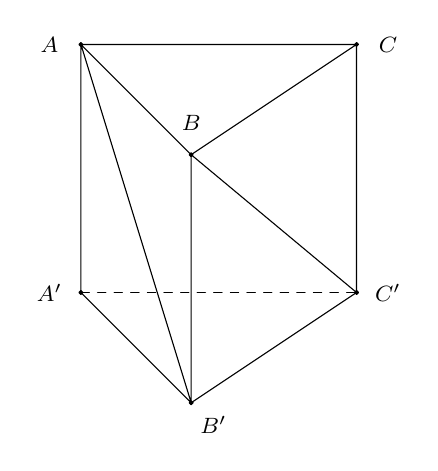
\begin{tikzpicture}[scale=0.7, font=\footnotesize, line join=round, line cap=round, >=stealth]
            \path
            (0,0) coordinate (A)
            (2,-2) coordinate (B)
            (5,0) coordinate (C) ;
            \foreach \x in {A,B,C}
            \path (\x)+(0,-4.5) coordinate(\x');
            \draw[dashed] (A')--(C');
            \draw (A')--(B')--(C') (A')--(A)--(B)--(C)--(C')--(B)--(B')--(A)--(C);
            \foreach \p/\g in {A/180,B/90,C/0,A'/180,B'/-45,C'/0}\draw[fill=black] (\p) circle (1pt)node[shift={(\g:.4)}]{$\p$};
    \end{tikzpicture}}
    \loigiai{
        Ta có
        \begin{eqnarray*}
            \overrightarrow{AB'}\cdot\overrightarrow{BC'}&= & \left(\overrightarrow{AB}+\overrightarrow{BB'}\right)\left(\overrightarrow{BC}+\overrightarrow{CC'}\right)\\
            &= & \overrightarrow{AB}\cdot\overrightarrow{BC}+\overrightarrow{AB}\cdot\overrightarrow{CC'}+\overrightarrow{BB'}\cdot\overrightarrow{BC}+\overrightarrow{BB'}\cdot\overrightarrow{CC'}\\
            &= & \overrightarrow{AB}\cdot\overrightarrow{BC}+\overrightarrow{AB}\cdot\overrightarrow{CC'}+\overrightarrow{BB'}\cdot\overrightarrow{BC}+\overrightarrow{BB'}\cdot\overrightarrow{CC'}\\
            &= & -\dfrac{a^2}{2}+0+0+2a^2=\dfrac{3a^2}{2}.
        \end{eqnarray*}
        Suy ra $\cos\left(\overrightarrow{AB'},\overrightarrow{BC'}\right)=\dfrac{\overrightarrow{AB'}\cdot\overrightarrow{BC'}}{\left|\overrightarrow{AB'}\right|\cdot\left|\overrightarrow{BC'}\right|} =\dfrac{\dfrac{3a^2}{2}}{a\sqrt{3}\cdot a\sqrt{3}}=\dfrac{1}{2}\Rightarrow\widehat{(AB',BC')}=60^{\circ}$.
    }
\end{ex}
%---------------------
\begin{ex}%%[1H3K2-4]
    [Kim Liên - Hà Nội - 2018]
    Cho tứ diện $ABCD$ có $DA=DB=DC=AC=AB=a$, $\widehat{ABC}=45^{\circ}$. Tính góc giữa hai đường thẳng $AB$ và $DC$.
    \choice
    {\True $60^{\circ}$}
    {$120^{\circ}$}
    {$90^{\circ}$}
    {$30^{\circ}$}
    \loigiai{
        Ta có tam giác $ABC$ vuông cân tại $A$, tam giác $BDC$ vuông cân tại $D$.\\
        Ta có
        \allowdisplaybreaks
        $\begin{aligned}[t]
            \vec{AB}\cdot\vec{CD}=\left(\vec{DB}-\vec{DA}\right)\vec{CD}&=\vec{DB}\cdot\vec{CD}-\vec{DA}\cdot\vec{CD}\\
            &=\left|\vec{DB}\right|\left|\vec{CD}\right|\cos\left(\vec{DB},\vec{CD}\right)-\left|\vec{DA}\right|\left|\vec{CD}\right|\cos\left(\vec{DA},\vec{CD}\right)\\
            &=-\dfrac{1}{2}a^2
        \end{aligned}$\\
        Mặt khác ta lại có $\cos\left(\vec{AB},\vec{CD}\right)=\dfrac{\vec{AB}\cdot\vec{CD}}{\left|\vec{AB}\right|\left|\vec{CD}\right|}=-\dfrac{1}{2}$\\
        Suy ra $\left(\vec{AB},\vec{DC}\right)=120^{\circ}\Rightarrow(AB,CD)=60^{\circ} $.
    }
\end{ex}
\begin{ex}%%[1H3K2-4]
    [Chuyên Trần Phú - Hải Phòng - 2018]
    Cho hình lập phương $ABCD.A'B'C'D'$. Gọi $M$, $N$ lần lượt là trung điểm của $AD$, $BB'$. Cosin của góc hợp bởi $MN$ và $AC'$ bằng
    \choice
    {$\dfrac{\sqrt{3}}{3}$}
    {\True $\dfrac{\sqrt{2}}{3}$}
    {$\dfrac{\sqrt{5}}{3}$}
    {$\dfrac{\sqrt{2}}{4}$}
    \loigiai{
        \begin{center}
            \begin{tikzpicture}[line cap=round,line join=round, >=stealth,scale=1]
                \def \a{-1.5} \def \b{-1}\def \c{4.5} \def \h{4}
                \path (.5,.5)coordinate(A)
                +(\a,\b)coordinate(B)
                +(\c,0)coordinate(D)
                ($(B)+(D)-(A)$)coordinate(C)
                +(0,\h) coordinate(C')
                ($(B)+(C')-(C)$)coordinate(B')
                ($(A)+(C')-(C)$)coordinate(A')
                ($(D)+(C')-(C)$)coordinate(D')
                ($(B)!.5!(B')$) coordinate (N)
                ($(A)!.5!(D)$) coordinate (M);
                \draw [dashed] (C')--(A)--(B)(D)--(A)--(A') (M)--(N);
                \draw (B')--(B)--(C)(B')--(C')--(C)--(D)--(D')--(A')--(B')(C')--(D');
                \foreach \x/\g in {A/135,B/-135,C/-45,D/0,A'/135,B'/180,C'/-20,D'/0,M/60,N/180}\fill[red] (\x) circle (1pt)+(\g:3mm) node[black]{$\x$};
            \end{tikzpicture}
        \end{center}
        Xét hình lập phương $ABCD.A'B'C'D'$ cạnh $a$.\\
        Đặt $\vec{a}=\vec{AB}$, $\vec{b}=\vec{AD}$, $\vec{c}=\vec{AA'}\Rightarrow\left|\vec{a}\right|=\left|\vec{b}\right|=\left|\vec{c}\right|=a$.\\
        Từ đó suy ra  $\vec{a}\cdot\vec{b}=\vec{b}\cdot\vec{c}=\vec{a}\cdot\vec{c}=0$.\\
        Ta có
        \begin{itemize}
            \item $\vec{MN}=\vec{AB}+\vec{BN}-\vec{AM}=\vec{a}-\dfrac{1}{2}\vec{b}+\dfrac{1}{2}\vec{c}\Rightarrow\left|\vec{MN}\right|=\sqrt{a^2+\dfrac{1}{4}a^2+\dfrac{1}{4}a^2}=\dfrac{a\sqrt{3}}{\sqrt{2}}$.
            \item $\vec{AC'}=\vec{AB}+\vec{AD}+\vec{AA'}=\vec{a}+\vec{b}+\vec{c}\Rightarrow\left|\vec{AC'}\right|=\sqrt{a^2+a^2+a^2}=a\sqrt{3}$.
            \item $\vec{AC'}\cdot\vec{MN}=a^2-\dfrac{1}{2}a^2+\dfrac{1}{2}a^2=a^2$.
        \end{itemize}
        Từ đso suy ra
        $\cos(MN;AC')=\left|\cos\left(\vec{MN};\vec{AC'}\right)\right|=\dfrac{\left|\vec{MN}\cdot\vec{AC'}\right|}{\left|\vec{MN}\right|\cdot\left|\vec{AC'}\right|}=\dfrac{\sqrt{2}}{3}$.
    }
\end{ex}
\begin{ex}%%[1H3K2-4]
    [Cụm 5 Trường Chuyên - ĐBSH - 2018]
    Cho hình chóp $S.ABCD$ có đáy là hình chữ nhật, $AB=2a$, $BC=a$. Hình chiếu vuông góc $H$ của đỉnh $S$ trên mặt phẳng đáy là trung điểm của cạnh $AB$, góc giữa đường thẳng $SC$ và mặt phẳng đáy bằng $60^{\circ}$. Tính cosin góc giữa hai đường thẳng $SB$ và $AC$
    \choice
    {$\dfrac{2}{\sqrt{7}}$}
    {\True $\dfrac{2}{\sqrt{35}}$}
    {$\dfrac{2}{\sqrt{5}}$}
    {$\dfrac{\sqrt{2}}{\sqrt{7}}$}
    \loigiai{
        \immini
        {
            Ta có $\left(SC,(ABCD)\right)= (SC,CH)=\widehat{SCH}=60^{\circ}$.\\
            %        $\cos(SB,AC)=\dfrac{\left|\vec{SB}\cdot\vec{AC}\right|}{SB\cdot AC}$.\\
            Ta có $AC=a\sqrt{5}$, $CH=\sqrt{a^2+a^2}=a\sqrt{2}$,\\ $SH=CH\cdot\tan\widehat{SCH}=a\sqrt{6}$
            \allowdisplaybreaks
            \begin{align*}
                \vec{SB}\cdot\vec{AC}&=\left(\vec{SH}+\vec{HB}\right)\left(\vec{AB}+\vec{BC}\right)\\ &=\vec{SH}\cdot\vec{AB}+\vec{SH}\cdot\vec{BC}+\vec{HB}\cdot\vec{AB}+\vec{HB}\cdot\vec{BC}\\
                &=\vec{HB}\cdot\vec{AB}+\vec{HB}\cdot\vec{BC} =\dfrac{1}{2}AB^2=2a^2.
            \end{align*}
            $SB=\sqrt{SH^2+HB^2} =\sqrt{(a\sqrt{6})^2+a^2}=a\sqrt{7}$.
        }
        {
            \begin{tikzpicture}[line cap=round,line join=round, >=stealth,scale=1]
                \def \a{-2} \def \b{-1} \def \c{4} \def \h{4}
                \path (0,0)coordinate(A)
                +(\a,\b)coordinate(B)
                +(\c,0)coordinate(D)
                ($(B)+(D)-(A)$)coordinate(C)
                ($(A)!1/2!(B)$)coordinate(H)
                +(0,\h)coordinate(S)
                ;
                \draw [dashed] (B)--(A)--(D) (A)--(S) (S)--(H)--(C)--(A);
                \draw (S)--(B)--(C)--(D)--(S)--(C)
                pic[draw,angle radius=2mm]{right angle=S--H--A}
                ;
                \foreach \x/\g in {A/160,B/-145,C/-45,D/0,S/90,H/145}\fill[draw,fill=white] (\x) circle (1pt)+(\g:3mm) node[black]{$\x$};
            \end{tikzpicture}
        }
        \noindent
        Vậy $\cos(SB,AC)=\dfrac{\vec{SB}\cdot\vec{AC}}{SB\cdot AC} =\dfrac{2a^2}{a\sqrt{7}\cdot a\sqrt{5}} =\dfrac{2}{\sqrt{35}}$.
    }
\end{ex}
\begin{ex}%[1H3B2-3]
    [Chuyên Thái Bình - 2018]%Câu 18.
    Cho hình chóp tứ giác đều $S.ABCD$ có đáy $ABCD$ là hình vuông, $E$ là điểm đối xứng của $D$ qua trung điểm $SA$. Gọi $M$, $N$ lần lượt là trung điểm của $AE$ và $BC$. Góc giữa hai đường thẳng $MN$ và $BD$ bằng
    \choice
    {\True $90^{\circ}$}
    {$60^{\circ}$}
    {$45^{\circ}$}
    {$75^{\circ}$}
    \loigiai{
        \begin{center}
            \begin{tikzpicture}[scale=1, font=\footnotesize, line join=round, line cap=round, >=stealth]
                \def\bc{4} % cạnh BC
                \def\ba{2} % cạnh BA
                \def\h{4} % đường cao
                \def\gocB{30} % góc B của đáy
                \path
                (0,0) coordinate (B)
                (\gocB:\ba) coordinate (A)
                (\bc,0) coordinate (C)
                ($(C)-(B)+(A)$) coordinate (D)
                ($(A)!.5!(C)$) coordinate (O)
                ($(O)+(90:\h)$) coordinate (S)
                ($(S)!.5!(A)$) coordinate (I)
                ($(I)!-1!(D)$) coordinate (E)
                ($(B)!.5!(C)$) coordinate (N)
                ($(A)!.5!(E)$) coordinate (M)
                \foreach \x/\y/\z/\t/\l in {E/D/S/B/ed,M/I/S/B/mi,M/N/S/B/mn,E/A/S/B/ea}
                {
                    (intersection of {\x}--{\y} and {\z}--{\t}) coordinate (\l)
                };
                \draw (B)--(C)--(D)--(S)--cycle (S)--(C)
                (ed)--(E)--(ea)
                (mi)--(M)--(mn);
                \draw[dashed] (C)--(A)--(D)--(B) (O)--(S)--(A)--(B)
                (D)--(ed)
                (C)--(I)--(mi)
                (N)--(mn)
                (A)--(ea);
                \foreach \x/\g in {A/30,B/-135,C/-45,D/0,O/-120,S/90,I/10,E/90,M/-150,N/-90}\fill[red] (\x) circle (1pt)+(\g:3mm) node[black]{$ \x $};
            \end{tikzpicture}
        \end{center}
        Gọi $I$ là trung điểm $SA$ thì $IMNC$ là hình bình hành nên $MN\parallel IC$.\\
        Ta có $BD\perp(SAC)\Rightarrow BD\perp IC$ mà $MN\parallel IC\Rightarrow BD\perp MN$ nên góc giữa hai đường thẳng $MN$ và $BD$ bằng $90^{\circ}$.\\
        \textbf{Cách khác:} có thể dùng hệ trục tọa độ của lớp 12, tính tích vô hướng $\vec{BD}\cdot\vec{MN}=0$.
    }
\end{ex}
\begin{ex}%[1H3B2-3]
    [Chuyên Thái Bình - 2018]%Câu 19.
    Cho hình chóp đều $S.ABCD$ có tất cả các cạnh đều bằng $a$. Gọi $M$, $N$ lần lượt là trung điểm của $AD$ và $SD$. Số đo của góc giữa hai đường thẳng $MN$ và $SC$ là
    \choice
    {$45^{\circ}$}
    {$60^{\circ}$}
    {$30^{\circ}$}
    {\True $90^{\circ}$}
    \loigiai{
        \immini
        {
            Ta có $MN \parallel SA$ ($MN$ là đường trung bình của $\triangle SAD$).\\
            Suy ra $(MN,SC)=(SA,SC)$.\\
            Trong $\triangle SAC$, có $SA=SC=a$ và $AC=a\sqrt{2}$\\
            Nên $\triangle SAC$ vuông cân tại $S$.\\
            Vậy $(MN,SC)=(SA,SC)=\widehat{ASC}=90^\circ$.
        }
        {
            \begin{tikzpicture}[scale=1, font=\footnotesize, line join=round, line cap=round, >=stealth]
                \def\bc{4} % cạnh BC
                \def\ba{2.2} % cạnh BA
                \def\h{4} % đường cao
                \def\gocB{30} % góc B của đáy
                \path
                (0,0) coordinate (B)
                (\gocB:\ba) coordinate (A)
                (\bc,0) coordinate (C)
                ($(C)-(B)+(A)$) coordinate (D)
                ($(A)!.5!(C)$) coordinate (O)
                ($(O)+(90:\h)$) coordinate (S)
                ($(D)!.5!(A)$) coordinate (M)
                ($(D)!.5!(S)$) coordinate (N);
                \draw (B)--(C)--(D)--(S)--cycle (S)--(C);
                \draw[dashed] (C)--(A)--(D)--(B) (O)--(S)--(A)--(B) (M)--(N);
                \foreach \x/\g in {A/120,B/-135,C/-45,D/0,O/-120,S/90,M/-40,N/60}\fill[red] (\x) circle (1pt)+(\g:3mm) node[black]{$ \x $};
            \end{tikzpicture}
        }
    }
\end{ex}
\begin{ex}%[1H3K2-3]
    [Sở Quảng Nam - 2018]%Câu 20.
    Cho hình lăng trụ $ABC.A'B'C'$ có đáy $ABC$ là tam giác vuông tại $A$, $AB=a$, $AC=a\sqrt{3}$. Hình chiếu vuông góc của $A'$ lên mặt phẳng $(ABC)$ là trung điểm $H$ của $BC$, $A'H=a\sqrt{3}$. Gọi $\varphi$ là góc giữa hai đường thẳng $A'B$ và $B'C$. Tính $\cos\varphi$.
    \choice
    {$\cos\varphi=\dfrac{1}{2}$}
    {\True $\cos\varphi=\dfrac{\sqrt{6}}{8}$}
    {$\cos\varphi=\dfrac{\sqrt{6}}{4}$}
    {$\cos\varphi=\dfrac{\sqrt{3}}{2}$}
    \loigiai{
        \begin{center}
            \begin{tikzpicture}[scale=1, font=\footnotesize, line join=round, line cap=round, >=stealth]
                \def\ac{5} % cạnh AC
                \def\ab{2.2} % cạnh AB
                \def\h{4} % chiều cao
                \def\gocA{30} % góc A của đáy
                \path
                (0,0) coordinate (A)
                (\ac,0) coordinate (C)
                (-\gocA:\ab) coordinate (B)
                ($(B)!.5!(C)$) coordinate (H)
                ($(H)+(90:\h)$) coordinate (A')
                ($(B)-(A)+(A')$) coordinate (B')
                ($(C)-(A)+(A')$) coordinate (C')
                ($(A)!.5!(C)$) coordinate (E)
                ($(B)!-1!(A)$) coordinate (D)
                ($(D)-(B)+(H)$) coordinate (K)
                (intersection of E--K and D--C) coordinate (ek);
                \draw (B)--(A')--(A)--(B) (C)--(C')--(A')--(B')--(C') (D)--(B)--(B')--(D)--(C)--(B')--(K)
                (C)--(K)--(ek);
                \draw[dashed] (A)--(C) (A')--(H)--(A) (B)--(C)
                (E)--(ek);
                \foreach \x/\g in {A/180,B/-90,C/130,A'/180,C'/0,B'/-40,D/-90,K/-40,H/-90,E/50}\fill[red] (\x) circle (1pt)+(\g:3mm) node[black]{$ \x $};
            \end{tikzpicture}
        \end{center}
        Gọi $E$ là trung điểm của $AC$; $D$ và $K$ là các điểm thỏa $\vec{BD}=\vec{HK}=\vec{A'B'}$.\\
        Ta có $B'K\perp(ABC)$ và $B'D\parallel A'B\Rightarrow(A'B,B'C)=(B'D,B'C) =\widehat{DB'C}$.\\
        Ta tính được $BC=2a\Rightarrow BH=a$; $B'D=A'B=\sqrt{(a\sqrt{3})^2+a^2}=2a$.\\
        $CD=\sqrt{AC^2+AD^2}=a\sqrt{7}$; $CK=\sqrt{CE^2+EK^2}=a\sqrt{3}$.\\
        $B'C=\sqrt{B'K^2+CK^2}=\sqrt{3a^2+3a^2}=a\sqrt{6}$.\\
        $\cos\widehat{CB'D}=\dfrac{B'D^2+B'C^2-CD^2}{2\cdot B'D\cdot B'C} =\dfrac{4a^2+6a^2-7a^2}{2\cdot 2a\cdot a\sqrt{6}}=\dfrac{\sqrt{6}}{8}$.
    }
\end{ex}
\begin{ex}%[1H3B2-3]
    [Sở Yên Bái - 2018]%Câu 21.
    Cho tứ diện đều $ABCD$, $M$ là trung điểm của cạnh $BC$. Tính giá trị của $\cos(AB,DM)$.
    \choice
    {$\dfrac{\sqrt{3}}{2}$}
    {\True $\dfrac{\sqrt{3}}{6}$}
    {$\dfrac{1}{2}$}
    {$\dfrac{\sqrt{2}}{2}$}
    \loigiai{
        \immini
        {
            Giả sử cạnh của tứ diện đều bằng $a$.\\
            Gọi $N$ là trung điểm của $AC$.\\
            Khi đó $\left(AB,DM\right)=\left(MN,DM\right)$.\\
            Ta có $MN=\dfrac{a}{2}$, $DM=DN=\dfrac{a\sqrt{3}}{2}$.\\
            $\cos\widehat{NMD}=\dfrac{MN^2+MD^2-ND^2}{2\cdot MN\cdot MD}=\dfrac{\dfrac{a^2}{4}}{2\cdot\dfrac{a}{2}\cdot\dfrac{a\sqrt{3}}{2}}=\dfrac{\sqrt{3}}{6}$.\\
            Vậy $\cos(AB,DM)=\dfrac{\sqrt{3}}{6}$.
        }
        {
            \begin{tikzpicture}[scale=1, font=\footnotesize, line join=round, line cap=round, >=stealth]
                \def\ac{4} % cạnh AC
                \def\ab{2} % cạnh AB
                \def\h{4} % chiều cao
                \def\gocA{50} % góc A của đáy
                \path
                (0,0) coordinate (D)
                (\ac,0) coordinate (C)
                (-\gocA:\ab) coordinate (B)
                ($(B)!.5!(C)$) coordinate (M)
                --(D) coordinate[pos=1/3](G)
                ($(G)+(90:\h)$) coordinate (A)
                ($(A)!.5!(C)$) coordinate (N)
                ;
                \draw (D)--(B)--(C)--(A)--cycle (A)--(B) (M)--(N);
                \draw[dashed] (N)--(D)--(M) (A)--(G) (C)--(D);
                \foreach \x/\g in {A/90,B/-90,C/0,D/180,M/-35,N/20}\fill[draw,fill=white] (\x) circle (1pt)+(\g:3mm) node[black]{$\x$};
            \end{tikzpicture}
        }
    }
\end{ex}
\begin{ex}%[1H3K2-4]
    [Sở Nam Định - 2018]%Câu 22.
    Cho hình lăng trụ $ABC.A'B'C'$ có đáy $ABC$ là tam giác đều cạnh $a$, tam giác $A'BC$ đều nằm trong mặt phẳng vuông góc với $(ABC)$. $M$ là trung điểm cạnh $CC'$. Tính cosin góc $\alpha$ giữa hai đường thẳng $AA'$ và $BM$.
    \choice
    {$\cos\alpha=\dfrac{2\sqrt{22}}{11}$}
    {\True $\cos\alpha=\dfrac{\sqrt{33}}{11}$}
    {$\cos\alpha=\dfrac{\sqrt{11}}{11}$}
    {$\cos\alpha=\dfrac{\sqrt{22}}{11}$}
    \loigiai{
        \immini
        {
            Ta có $AH=A'H=\dfrac{a\sqrt{3}}{2}$ và $AH\perp BC$, $A'H\perp BC$.\\
            Suy ra $BC\perp(AA'H)\Rightarrow BC\perp AA'$ hay $BC\perp BB'$.\\
            Do đó $BCC'B'$ là hình chữ nhật.\\
            Khi đó $CC'=AA'=\dfrac{a\sqrt{3}}{2}\cdot\sqrt{2}=\dfrac{a\sqrt{6}}{2}$.\\
            $ BM=\sqrt{a^2+\dfrac{a^2\cdot 6}{16}}=a\dfrac{\sqrt{22}}{4}$.\\
            Xét $\vec{AA'}\cdot\vec{BM}=\vec{AA'}\cdot\left(\vec{BC}+\vec{CM}\right)=\dfrac{3a^2}{4}$.\\
            Suy ra $\cos(AA',BM)=\dfrac{\left|\dfrac{3a^2}{4}\right|}{\dfrac{a\sqrt{6}}{2}\cdot\dfrac{a\sqrt{22}}{4}} =\dfrac{\sqrt{33}}{11}$.
        }
        {
            \begin{tikzpicture}[scale=1, font=\footnotesize, line join=round, line cap=round, >=stealth]
                \def\ac{3} % cạnh AC
                \def\ab{1.6} % cạnh AB
                \def\h{3.5} % chiều cao
                \def\gocA{60} % góc A của đáy
                \path
                (0,0) coordinate (A)
                (\ac,0) coordinate (C)
                (-\gocA:\ab) coordinate (B)
                ($(B)!.5!(C)$) coordinate (H)
                ($(H)+(90:\h)$) coordinate (A')
                ($(B)-(A)+(A')$) coordinate (B')
                ($(C)-(A)+(A')$) coordinate (C')
                ($(C)!.5!(C')$) coordinate (M);
                \draw (A')--(A)--(B)--(C)--(C')--(A')--(B')--(C') (M)--(B)--(B');
                \draw[dashed] (A)--(C) (A)--(H)--(A')
                (A')--(C);
                \foreach \x/\g in {A/180,B/-90,C/0,A'/180,C'/0,B'/-40,H/-50,M/-10}\fill[red] (\x) circle (1pt)+(\g:3mm) node[black]{$ \x $};
            \end{tikzpicture}
        }
    }
\end{ex}
\begin{ex}[Sở Hà Tĩnh - 2018]%Câu 23.%[1H3B2-3]
    Cho hình lăng trụ tam giác đều $ABC.MNP$ có tất cả các cạnh bằng nhau. Gọi $I$ là trung điểm cạnh $AC$. Côsin của góc giữa hai đường thẳng $NC$ và $BI$ bằng
    \choice
    {\True $\dfrac{\sqrt{6}}{4}$}
    {$\dfrac{\sqrt{15}}{5}$}
    {$\dfrac{\sqrt{6}}{2}$}
    {$\dfrac{\sqrt{10}}{4}$}
    \loigiai{
        \immini
        {
            Giả sử các cạnh của lăng trụ bằng $a$.\\
            Gọi $K$ là trung điểm của $MP$.\\
            Suy ra $ BI\parallel NK\Rightarrow(NC,BI)=(NC,NK)$.\\
            Vì $ABC.MNP$ là lăng trụ tam giác đều $\Rightarrow CP\perp(MNP)$.\\
            $CK=\sqrt{CP^2+PK^2} =\dfrac{a\sqrt{5}}{2}$.\\
            $CN=\sqrt{CP^2+NP^2} =a\sqrt{2}$.\\
            $NK=\sqrt{NP^2-KP^2} =\dfrac{a\sqrt{3}}{2}$.\\
            Vậy $\cos\widehat{CNK}=\dfrac{NC^2+NK^2-CK^2}{2NC\cdot NK} =\dfrac{\sqrt{6}}{4}$.
        }
        {
            \begin{tikzpicture}[scale=1, font=\footnotesize, line join=round, line cap=round, >=stealth]
                \def\ac{5} % cạnh AC
                \def\ab{4} % cạnh AB
                \def\h{5} % chiều cao
                \def\gocA{30} % góc A của đáy
                \path
                (0,0) coordinate (A)
                (\ac,0) coordinate (C)
                (-\gocA:\ab) coordinate (B)
                ($(A)+(-90:\h)$) coordinate (M)
                ($(B)-(A)+(M)$) coordinate (N)
                ($(C)-(A)+(M)$) coordinate (P)
                ($(M)!.5!(P)$) coordinate (K)
                ($(A)!.5!(C)$) coordinate (I);
                \draw (M)--(N)--(P)--(M)--(A)--(B)--(C)--(P) (B)--(N)--(C)--(A) (B)--(I);
                \draw[dashed] (M)--(P) (C)--(K)--(N);
                \foreach \x/\g in {A/180,B/-150,C/0,M/180,N/-90,P/-40,I/90,K/120}\fill[red] (\x) circle (1pt)+(\g:3mm) node[black]{$ \x $};
            \end{tikzpicture}
        }
    }
\end{ex}
\begin{ex}[Chuyên Biên Hòa - Hà Nam - 2020]%Câu 24.%[1H3B2-3]
    Cho tứ diện đều $ABCD$, $M$ là trung điểm của cạnh $BC$. Khi đó $\cos(AB, DM)$ bằng
    \choice
    {$\dfrac{\sqrt{2}}{2}$}
    {\True $\dfrac{\sqrt{3}}{6}$}
    {$\dfrac{1}{2}$}
    {$\dfrac{\sqrt{3}}{2}$}
    \loigiai{
        \immini
        {
            Gọi $N$ là trung điểm của $AC$. Suy ra $MN\parallel AB$.\\
            Do đó $\cos(AB, DM)=\cos(MN, DM)$.\\
            Gọi $a$ là độ dài cạnh của tứ diện đều $ABCD$.\\
            Suy ra $MN=\dfrac{a}{2}$; $ND=MD=\dfrac{a\sqrt{3}}{2}$.\\
            Trong tam giác $MND$ ta có \[\cos\widehat{NMD}=\dfrac{MN^2+MD^2-ND^2}{2\cdot MN\cdot MD}=\dfrac{\sqrt{3}}{6}.\]
            Vậy $\cos(AB, DM)=\cos\widehat{NMD}=\dfrac{\sqrt{3}}{6}$.
        }
        {
            \begin{tikzpicture}[scale=1, font=\footnotesize, line join=round, line cap=round, >=stealth]
                \def\ac{4}
                \def\ab{2}
                \def\h{4}
                \def\gocA{50}
                \path
                (0,0) coordinate (D)
                (\ac,0) coordinate (C)
                (-\gocA:\ab) coordinate (B)
                ($(B)!.5!(C)$) coordinate (M)
                --(D) coordinate[pos=1/3](G)
                ($(G)+(90:\h)$) coordinate (A)
                ($(A)!.5!(C)$) coordinate (N)
                ;
                \draw (D)--(B)--(C)--(A)--cycle (A)--(B) (M)--(N);
                \draw[dashed] (N)--(D)--(M) (C)--(D);
                \foreach \x/\g in {A/90,B/-90,C/0,D/180,M/-35,N/20}\fill[draw,fill=white] (\x) circle (1pt)+(\g:3mm) node[black]{$\x$};
            \end{tikzpicture}
        }
    }
\end{ex}
\begin{ex}[ĐHQG Hà Nội - 2020]%Câu 25.%[2H3B4-1]
    Cho hình chóp $S.ABCD$ có đáy hình vuông. Cho tam giác $SAB$ vuông tại $S$ và góc $SBA$ bằng $30^{\circ}$. Mặt phẳng $(SAB)$ vuông góc mặt phẳng đáy. Gọi $M,N$ là trung điểm $AB,BC$. Tìm cosin góc tạo bởi hai đường thẳng $(SM,DN)$.
    \choice
    {$\dfrac{2}{\sqrt{5}}$}
    {\True $\dfrac{1}{\sqrt{5}}$}
    {$\dfrac{1}{\sqrt{3}}$}
    {$\dfrac{\sqrt{2}}{\sqrt{3}}$}
    \loigiai{
        Trong $(SAB)$, kẻ $SH\perp AB$ tại $H$. Ta có: $\heva{&(SAB)\perp(ABCD)\\&(SAB)\cap(ABCD)=AB\\&SH\subset(SAB),SH\perp AB}\Rightarrow SH\perp(ABCD)$.\\
        Kẻ tia $Az\parallel SH$ và chọn hệ trục tọa độ $Axyz$ như hình vẽ sau đây.
        \begin{center}
            \begin{tikzpicture}[line cap=round,line join=round, >=stealth,scale=1]
                \def \a{-2} \def \b{-1} \def \c{4} \def \h{4}
                \path (0,0)coordinate(A)
                +(\a,\b)coordinate(B)
                +(\c,0)coordinate(D)
                ($(B)+(D)-(A)$)coordinate(C)
                ($(A)!1/2!(B)$)coordinate(H)
                +(0,\h)coordinate(S)
                (A)--(B)--([turn]0:1)coordinate (y)node[below right]{$y$}
                (A)--(D)--([turn]0:1)coordinate (x)node[below]{$x$}
                ($(A)+(90:.1)$) coordinate (zz)
                (intersection of A--zz and S--D) coordinate (zzz)
                ($(B)!.5!(C)$) coordinate (N)
                ;
                \draw[->] (B)--(y);
                \draw[->] (D)--(x);
                \draw[->] (zzz)--++(90:1)node[above left]{$z$};
                \draw [dashed] (B)--(A)--(D)--(N) (A)--(S) (S)--(H) (A)--(zzz);
                \draw (S)--(B)--(C)--(D)--(S)--(C)
                pic[draw,angle radius=2mm]{right angle=S--H--A}
                ;
                \foreach \x/\g in {A/160,B/-65,C/-45,D/-60,S/90,H/145,N/-90}\fill[draw,fill=white] (\x) circle (1pt)+(\g:3mm) node[black]{$\x$};
            \end{tikzpicture}
        \end{center}
        Trong tam giác $SAB$ vuông tại $S$, $SB=AB\cdot\cos\widehat{SBA}=a\cdot\cos 30^{\circ}=\dfrac{a\sqrt{3}}{2}$.\\
        Trong tam giác $SBH$ vuông tại $H$, $BH=SB\cdot\cos\widehat{SBH}=\dfrac{3a}{4}$ và $SH=BH\cdot\sin\widehat{SBA}=\dfrac{a\sqrt{3}}{4}$.\\
        Ta có $AH=AB-BH=a-\dfrac{3a}{4}=\dfrac{a}{4}$. Suy ra $ H\left(0;\dfrac{a}{4};0\right)\Rightarrow S\left(0;\dfrac{a}{4};\dfrac{a\sqrt{3}}{4}\right)$.\\
        $M\left(0;\dfrac{a}{2};0\right)$, $D(a;0;0)$, $N\left(\dfrac{a}{2};a;0\right)$.\\
        Ta có $\vec{SM}=\left(0;\dfrac{a}{4};-\dfrac{a\sqrt{3}}{4}\right)$, $\vec{DN}=\left(-\dfrac{a}{2};a;0\right)$.
        \[\cos(SM,DN)=\dfrac{\left|\vec{SM}\cdot\vec{DN}\right|}{SN\cdot DN}=\dfrac{\dfrac{a^2}{4}}{\dfrac{a}{2}\cdot\dfrac{a\sqrt{5}}{2}}=\dfrac{1}{\sqrt{5}}.\]
    }
\end{ex}
\begin{ex}[Đề minh họa 2022]%Câu 26.%[1H3B2-3]
    \immini
    {
        Cho hình hộp $ABCD.A'B'C'D'$ có tất cả các cạnh bằng nhau (tham khảo hình bên).
        Góc giữa hai đường thẳng $A'C'$ và $BD$ bằng
        \choice
        {\True $90^{\circ}$}
        {$30^{\circ}$}
        {$45^{\circ}$}
        {$60^{\circ}$}
    }
    {
        \begin{tikzpicture}[line cap=round,line join=round, >=stealth,scale=.7]
            \def \a{-1.5} \def \b{-1}\def \c{4.5} \def \h{4}
            \path (.5,.5)coordinate(A)
            +(\a,\b)coordinate(B)
            +(\c,0)coordinate(D)
            ($(B)+(D)-(A)$)coordinate(C)
            +(0,\h) coordinate(C')
            ($(B)+(C')-(C)$)coordinate(B')
            ($(A)+(C')-(C)$)coordinate(A')
            ($(D)+(C')-(C)$)coordinate(D');
            \draw [dashed] (A)--(B)(D)--(A)--(A');
            \draw (B')--(B)--(C)(B')--(C')--(C)--(D)--(D')--(A')--(B')(C')--(D');
            \foreach \x/\g in {A/135,B/-135,C/-45,D/0,A'/135,B'/180,C'/-20,D'/0}\fill[red] (\x) circle (1pt)+(\g:3mm) node[black]{$\x$};
        \end{tikzpicture}
    }
    \loigiai{
        Ta có $A'C'\parallel AC$ nên $(A'C';BD)=(AC;BD)=90^{\circ}$.
    }
\end{ex}
\begin{dang}
	{Góc của đường thẳng với mặt phẳng}
\end{dang}
\begin{ex}[Đề Minh Hoạ 2021]%%[1H3B3-3]
    \immini{
        Cho hình hộp chữ nhật $ABCD.A’B’C’D’$ có $AB=AD=2$, $AA’=2\sqrt{2}$ (tham khảo hình vẽ bên). Góc giữa đường thẳng $CA’$ và mặt phẳng $(ABCD)$ bằng
        \choice
        {$30^{\circ}$}
        {\True $45^{\circ}$}
        {$60^{\circ}$}
        {$90^{\circ}$}
    }{
        \begin{tikzpicture}[scale=1]
            \path
            (0,0) coordinate (A)
            (-1,-0.8) coordinate (B)
            (1.5,-0.8) coordinate (C)
            ;
            \coordinate (D) at ($(A)+(C)-(B)$);
            \foreach \x / \y in {A'/A,B'/B, C'/C, D'/D}
            \coordinate (\x) at ($(\y)+(0,2)$);
            \draw (A') node [above] {$A'$} -- (B') node [left] {$B'$} -- (C') node [above] {$C'$} -- (D') node [above] {$D'$} -- (D) node [right] {$D$} -- (C)  node [below] {$C$}-- (B) node [below] {$B$} -- (B') 		(C) -- (C') (A') -- (D');
            \draw [dashed] (A') -- (A) node [left] {$A$} -- (D) (A) -- (B) (A') -- (C) -- (A);
            \foreach \x in {A,B,C,D,A',B',C',D'}
            \draw [fill=black] (\x) circle (0.4mm);
        \end{tikzpicture}
    }
    \loigiai{
        Vì $AA’\perp (ABCD)$ nên góc giữa đường thẳng $CA’$ và mặt phẳng $(ABCD)$ bằng góc $\widehat{A’CA}$.\\
        Ta có $AC=\sqrt{AB^2+BC^2}=2\sqrt{2}$.\\
        Khi đó ta có $\tan\widehat{A’CA}=\dfrac{AA’}{AC}=\dfrac{2\sqrt{2}}{2\sqrt{2}}=1$.\\
        Vậy số đo góc $\widehat{A’CA}=45^{\circ}$.
    }
\end{ex}
\begin{ex}%[1H3B3-3]
    [Đề Minh Hoạ 2020 lần 1]
    \immini{
        Cho hình chóp $S.ABCD$ có đáy là hình vuông cạnh $a\sqrt{3}$, $SA$ vuông góc với mặt phẳng đáy và $SA=2a$. Góc giữa $SC$ và mặt phẳng $(ABCD)$ bằng
        \choice
        {$45^{\circ}$}
        {$60^{\circ}$}
        {\True $30^{\circ}$}
        {$90^{\circ}$}
    }{
        \begin{tikzpicture}[scale=0.8]
            \path (0,0) coordinate (A) -- (4,0) coordinate (D) -- (-1.5,-1) coordinate (B) -- (0,3) coordinate (S);
            \coordinate (C) at ($(B)+(D)-(A)$);
            \draw (B) -- (C) --(D) -- (S) node [above] {$S$} -- (B) node [below] {$B$} (S) -- (C) node [below] {$C$};
            \draw [dashed] (A) -- (B) (S) -- (A) node [left] {$A$} -- (D) node [right] {$D$};
            \foreach \x in {S,A,B,C,D} \draw [fill=black] (\x) circle (0.4 mm);
        \end{tikzpicture}
    }
    \loigiai{
        Ta có $SA\perp (ABCD)$ nên $\left(\widehat{SC,(ABCD)}\right)=\widehat{SCA}$.\\
        $\tan\widehat{SCA}=\dfrac{SA}{AC}=\dfrac{a \cdot \sqrt{2}}{a \cdot \sqrt{3} \cdot \sqrt{2}}=\dfrac{1}{\sqrt{3}}\Rightarrow\widehat{SCA}=30^{\circ}$.
    }
\end{ex}

\begin{ex}%[1H3B3-3]
    [Đề Tham Khảo 2020 Lần 2]
    \immini{
        Cho hình chóp $S.ABC$ có $SA$ vuông góc với mặt phẳng $(ABCD)$, $SA=a\sqrt{2}$, tam giác $ABC$ vuông cân tại $B$ và $AC=2a$ (minh hoạ hình bên). Góc giữa đường thẳng $SB$ và mặt phẳng $(ABC)$ bằng
        \choice
        {$30^{\circ}$}
        {\True $45^{\circ}$}
        {$60^{\circ}$}
        {$90^{\circ}$}
    }{
        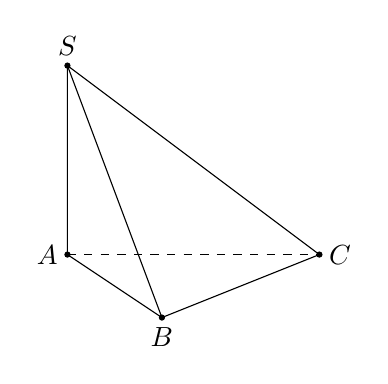
\begin{tikzpicture}[scale=0.8]
            \path (0,0) coordinate (A) -- (4,0) coordinate (C) -- (1.5,-1) coordinate (B) -- (0,3) coordinate (S);
            \draw (A) -- (B) -- (C) -- (S) -- (A) (S) node [above] {$S$} -- (B) node [below] {$B$};
            \draw [dashed] (A) node [left] {$A$} -- (C) node [right] {$C$};
            \foreach \x in {S,A,B,C} \draw [fill=black] (\x) circle (0.4 mm);
        \end{tikzpicture}
    }
    \loigiai{
        Ta có $\heva{&SB \cap (ABC)\\&SA\perp (ABC)} \Rightarrow AB$ là hình chiếu của $SB$ lên mặt phẳng $(ABC)$.\\
        Do đó $\left(\widehat{SB,(ABC)}\right)=\widehat{SBA}$.\\
        Do tam giác $ABC$ vuông cân tại $B$ suy ra $AB=\dfrac{AC}{\sqrt{2}}=a\sqrt{2}$.\\
        Xét tam giác $SAB$ vuông tại $A$, có $SA=AB=a\sqrt{2}$.\\
        Suy ra $\triangle SAB$ vuông cân tại $A$ và $\widehat{SBA}=45^{\circ}$.\\
        Vậy góc giữa đường thẳng $SB$ và mặt phẳng $ABC$ bằng $45^{\circ}$.
    }
\end{ex}

\begin{ex}%[1H3B3-3]
    [Mã 101 – 2020 Lần 1]
    \immini{
        Cho hình chóp $S.ABC$ có đáy $ABC$ là tam giác vuông tại $B$, $AB=a$, $BC=2a$, $SA$ vuông góc với mặt phẳng đáy và $SA=a\sqrt{15}$ (tham khảo hình bên). Góc giữa đường thẳng $SC$ và mặt phẳng đáy bằng
        \choice
        {$45^{\circ}$}
        {$30^{\circ}$}
        {\True $60^{\circ}$}
        {$90^{\circ}$}
    }{
        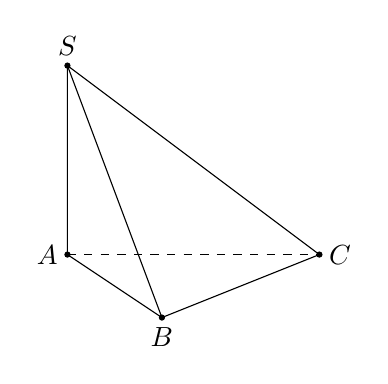
\begin{tikzpicture}[scale=0.8]
            \path (0,0) coordinate (A) -- (4,0) coordinate (C) -- (1.5,-1) coordinate (B) -- (0,3) coordinate (S);
            \draw (A) -- (B) -- (C) -- (S) -- (A) (S) node [above] {$S$} -- (B) node [below] {$B$};
            \draw [dashed] (A) node [left] {$A$} -- (C) node [right] {$C$};
            \foreach \x in {S,A,B,C} \draw [fill=black] (\x) circle (0.4 mm);
        \end{tikzpicture}
    }
    \loigiai{
        Do $SA$ vuông góc với mặt phẳng đáy nên $AC$ là hình chiếu vuông góc của $SC$ lên mặt phẳng đáy. Từ đó suy ra $\left(\widehat{SC,(ABC)}\right)=\left(\widehat{SC,AC}\right)=\widehat{SCA}$.\\
        Trong tam giác $ABC$ vuông tại $B$ ta có $AC=\sqrt{AB^2+BC^2}=\sqrt{a^2+4a^2}=a\sqrt{5}$.\\
        Trong tam giác $SAC$ vuông tại $A$ ta có $\tan\widehat{SCA}=\dfrac{SA}{AC}=\dfrac{a\sqrt{15}}{a\sqrt{5}}=\sqrt{3}\Rightarrow \widehat{SCA}=60^{\circ}$.\\
        Vậy $\left(\widehat{SC,(ABC)}\right)=60^{\circ}$.
    }
\end{ex}

\begin{ex}%[1H3B3-3]
    [Mã 102 – 2020 Lần 1]
    \immini{
        Cho hình chóp $S.ABC$ có đáy là tam giác vuông tại $B$, $AB=3a$, $BC=a\sqrt{3}$, $SA$ vuông góc với mặt phẳng đáy và $SA=2a$ (tham khảo hình vẽ). Góc giữa đường thẳng $SC$ và mặt phẳng đáy bằng
        \choice
        {$60^{\circ}$}
        {$45^{\circ}$}
        {\True $30^{\circ}$}
        {$90^{\circ}$}
    }{
        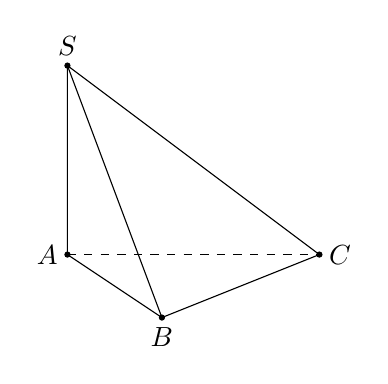
\begin{tikzpicture}[scale=0.8]
            \path (0,0) coordinate (A) -- (4,0) coordinate (C) -- (1.5,-1) coordinate (B) -- (0,3) coordinate (S);
            \draw (A) -- (B) -- (C) -- (S) -- (A) (S) node [above] {$S$} -- (B) node [below] {$B$};
            \draw [dashed] (A) node [left] {$A$} -- (C) node [right] {$C$};
            \foreach \x in {S,A,B,C} \draw [fill=black] (\x) circle (0.4 mm);
        \end{tikzpicture}
    }
    \loigiai{
        Vì $SA$ vuông góc với mặt phẳng đáy nên $AC$ là hình chiếu vuông góc của $SC$ lên đáy.\\
        Suy ra $\left(\widehat{SC,(ABC)}\right)=\left(\widehat{SC,AC}\right)=\widehat{SCA}$.
        \[\tan \widehat{SCA}=\dfrac{SA}{AC}=\dfrac{2a}{\sqrt{(3a)^2+(a\sqrt{3})^2}}=\dfrac{\sqrt{3}}{3}\Rightarrow\widehat{SCA}=30^{\circ}.\]
        Vậy $\left(\widehat{SC,(ABC)}\right)=30^{\circ}$.
    }
\end{ex}

\begin{ex}%[1H3B3-3]
    [Mã 103 – 2020 Lần 1]
    \immini{
        Cho hình chóp $S.ABC$ có đáy $ABC$ là tam giác vuông tại $B$, $AB=a$, $BC=3a$, $SA$ vuông góc với mặt phẳng đáy và $SA=a\sqrt{30}$ (tham khảo hình bên). Góc giữa đường thẳng $SC$ và mặt phẳng đáy bằng
        \choice
        {$45^{\circ}$}
        {$90^{\circ}$}
        {\True $60^{\circ}$}
        {$30^{\circ}$}
    }{
        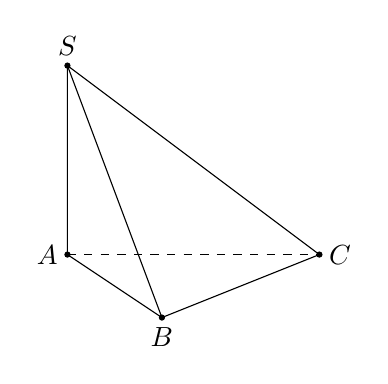
\begin{tikzpicture}[scale=0.8]
            \path (0,0) coordinate (A) -- (4,0) coordinate (C) -- (1.5,-1) coordinate (B) -- (0,3) coordinate (S);
            \draw (A) -- (B) -- (C) -- (S) -- (A) (S) node [above] {$S$} -- (B) node [below] {$B$};
            \draw [dashed] (A) node [left] {$A$} -- (C) node [right] {$C$};
            \foreach \x in {S,A,B,C} \draw [fill=black] (\x) circle (0.4 mm);
        \end{tikzpicture}
    }
    \loigiai{
        Do $AC$ là hình chiếu vuông góc với SC trên mặt phẳng $(ABC)$ nên $\left(\widehat{SC,(ABC)}\right)=\widehat{SCA}$.\\
        Ta có $AC=\sqrt{AB^2+BC^2}=a\sqrt{10}$.\\
        Khi đó $\tan\widehat{SCA}=\dfrac{SA}{AC}=\dfrac{a\sqrt{30}}{a\sqrt{10}}=\sqrt{3}\Rightarrow \widehat{SCA}=60^{\circ}$.\\
        Vậy góc giữa đường thẳng $SC$ và mặt phẳng đáy bằng $60^{\circ}$.
    }
\end{ex}

\begin{ex}%[1H3B3-3]
    [Mã 104 – 2020 Lần 1]
    \immini{
        Cho hình chóp $S.ABC$ có đáy $ABC$ là tam giác vuông tại $B$, $AB=a$, $BC=a\sqrt{2}$, $SA$ vuông góc với mặt phẳng đáy và $SA=a$ (tham khảo hình bên). Góc giữa đường thẳng $SC$ và mặt phẳng đáy bằng
        \choice
        {$90^{\circ}$}
        {$45^{\circ}$}
        {$60^{\circ}$}
        {\True $30^{\circ}$}
    }{
        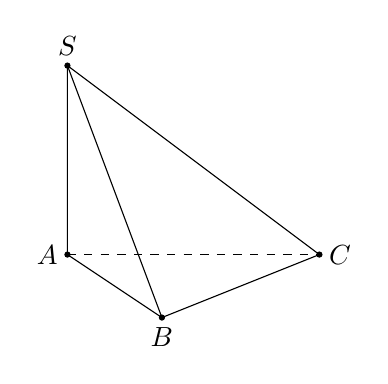
\begin{tikzpicture}[scale=0.8]
            \path (0,0) coordinate (A) -- (4,0) coordinate (C) -- (1.5,-1) coordinate (B) -- (0,3) coordinate (S);
            \draw (A) -- (B) -- (C) -- (S) -- (A) (S) node [above] {$S$} -- (B) node [below] {$B$};
            \draw [dashed] (A) node [left] {$A$} -- (C) node [right] {$C$};
            \foreach \x in {S,A,B,C} \draw [fill=black] (\x) circle (0.4 mm);
        \end{tikzpicture}
    }
    \loigiai{
        Ta có góc giữa $SC$ và đáy là $\widehat{SCA}$.\\
        Xét tam giác $SCA$ vuông tại $A$ có $AC=\sqrt{AB^2+BC^2}=a\sqrt{3}$.\\
        $\tan\widehat{SCA}=\dfrac{SA}{AC}=\dfrac{a}{a\sqrt{3}}\Rightarrow \widehat{SCA}=30^{\circ}$.
    }
\end{ex}

\begin{ex}%[1H3B3-3]
    [Mã 101 – 2020 Lần 2]
    \immini{
        Cho hình hộp chữ nhật $ABCD.A’B’C’D’$ có $AB=BC=a$, $A’A=a\sqrt{6}$ (tham khảo hình bên). Góc giữa đường thẳng $A’C$ và mặt phẳng $(ABCD)$ bằng
        \choice
        {\True $60^{\circ}$}
        {$90^{\circ}$}
        {$30^{\circ}$}
        {$45^{\circ}$}
    }{
        \begin{tikzpicture}[scale=1]
            \path
            (0,0) coordinate (A)
            (-1,-0.8) coordinate (B)
            (1.5,-0.8) coordinate (C)
            ;
            \coordinate (D) at ($(A)+(C)-(B)$);
            \foreach \x / \y in {A'/A,B'/B, C'/C, D'/D}
            \coordinate (\x) at ($(\y)+(0,2)$);
            \draw (A') node [above] {$A'$} -- (B') node [left] {$B'$} -- (C') node [above] {$C'$} -- (D') node [above] {$D'$} -- (D) node [right] {$D$} -- (C)  node [below] {$C$}-- (B) node [below] {$B$} -- (B') 		(C) -- (C') (A') -- (D');
            \draw [dashed] (A') -- (A) node [left] {$A$} -- (D) (A) -- (B) (A') -- (C) -- (A);
            \foreach \x in {A,B,C,D,A',B',C',D'}
            \draw [fill=black] (\x) circle (0.4mm);
            \node at ($(A)!0.35!(C)$) [below] {\tiny $a\sqrt{2}$};
            \node at ($(A)!0.35!(A')$) [above,rotate=90] {\tiny $a\sqrt{6}$};
        \end{tikzpicture}
    }
    \loigiai{
        \immini{
            Ta có góc giữa đường thẳng $A’C$ và mặt phẳng $(ABCD)$ bằng góc giữa $A’C$ và $AC$ là $\widehat{A’CA}$.\\
            Ta có $AC=\sqrt{AB^2+BC^2}=a\sqrt{2}$.\\
            Xét tam giác $A’CA$ có
            \[\tan\widehat{A’CA}=\dfrac{A’A}{AC}=\dfrac{a\sqrt{6}}{a\sqrt{2}}=\sqrt{3}\Rightarrow \widehat{A’CA}=60^{\circ}.\]
            Vậy góc $A’C$ và mặt phẳng $(ABCD)$ bằng $60^{\circ}$.
        }{
            \begin{tikzpicture}[scale=1]
                \path
                (0,0) coordinate (A)
                (-1,-0.8) coordinate (B)
                (1.5,-0.8) coordinate (C)
                ;
                \coordinate (D) at ($(A)+(C)-(B)$);
                \foreach \x / \y in {A'/A,B'/B, C'/C, D'/D}
                \coordinate (\x) at ($(\y)+(0,2)$);
                \draw (A') node [above] {$A'$} -- (B') node [left] {$B'$} -- (C') node [above] {$C'$} -- (D') node [above] {$D'$} -- (D) node [right] {$D$} -- (C)  node [below] {$C$}-- (B) node [below] {$B$} -- (B') 		(C) -- (C') (A') -- (D');
                \draw [dashed] (A') -- (A) node [left] {$A$} -- (D) (A) -- (B) (A') -- (C) -- (A);
                \foreach \x in {A,B,C,D,A',B',C',D'}
                \draw [fill=black] (\x) circle (0.4mm);
                \node at ($(A)!0.35!(C)$) [below] {\tiny $a\sqrt{2}$};
                \node at ($(A)!0.35!(A')$) [above,rotate=90] {\tiny $a\sqrt{6}$};
            \end{tikzpicture}
        }
    }
\end{ex}

\begin{ex}%[1H3B3-3]
    [Mã 102 – 2020 Lần 2]
    \immini{
        Cho hình hộp chữ nhật $ABCD.A’B’C’D’$ có $AB=a$, $AD=2a\sqrt{2}$, $A’A=a\sqrt{3}$ (tham khảo hình bên). Góc giữa đường thẳng $A’C$ và mặt phẳng $(ABCD)$ bằng
        \choice
        {\True $45^{\circ}$}
        {$90^{\circ}$}
        {$60^{\circ}$}
        {$30^{\circ}$}
    }{
        \begin{tikzpicture}[scale=1]
            \path
            (0,0) coordinate (A)
            (-1,-0.8) coordinate (B)
            (1.5,-0.8) coordinate (C)
            ;
            \coordinate (D) at ($(A)+(C)-(B)$);
            \foreach \x / \y in {A'/A,B'/B, C'/C, D'/D}
            \coordinate (\x) at ($(\y)+(0,2)$);
            \draw (A') node [above] {$A'$} -- (B') node [left] {$B'$} -- (C') node [above] {$C'$} -- (D') node [above] {$D'$} -- (D) node [right] {$D$} -- (C)  node [below] {$C$}-- (B) node [below] {$B$} -- (B') 		(C) -- (C') (A') -- (D');
            \draw [dashed] (A') -- (A) node [left] {$A$} -- (D) (A) -- (B) (A') -- (C);
            \foreach \x in {A,B,C,D,A',B',C',D'}
            \draw [fill=black] (\x) circle (0.4mm);
        \end{tikzpicture}
    }
    \loigiai{
        Ta thấy hình chiếu của $A’C$ xuống $(ABCD)$ là $AC$ do đó $\left(A’C,(ABCD)\right)=(A’C,AC)=\widehat{A’CA}$.\\
        Ta có $AC=\sqrt{AB^2+AD^2}=3a$.\\
        Xét tam giác $A’CA$ vuông tại $C$ ta có $\tan\widehat{A’CA}=\dfrac{A’A}{AC}=\dfrac{a\sqrt{3}}{3a}=\dfrac{\sqrt{3}}{3}$. Suy ra $\widehat{A’CA}=30^{\circ}$.\\
        Vậy $\left(\widehat{A’C,(ABCD)}\right)=\widehat{A’CA}=30^{\circ}$.
    }
\end{ex}

\begin{ex}%[1H3B3-3]
    [Mã 103 – 2020 Lần 2]
    \immini{
        Cho hình hộp chữ nhật $ABCD.A’B’C’D’$ có $AB=AA’=a$, $AD=a\sqrt{2}$ (tham khảo hình bên). Góc giữa đường thẳng $A’C$ và mặt phẳng $(ABCD)$ bằng
        \choice
        {\True $30^{\circ}$}
        {$45^{\circ}$}
        {$90^{\circ}$}
        {$60^{\circ}$}
    }{
        \begin{tikzpicture}[scale=1]
            \path
            (0,0) coordinate (A)
            (-1,-0.8) coordinate (B)
            (1.5,-0.8) coordinate (C)
            ;
            \coordinate (D) at ($(A)+(C)-(B)$);
            \foreach \x / \y in {A'/A,B'/B, C'/C, D'/D}
            \coordinate (\x) at ($(\y)+(0,2)$);
            \draw (A') node [above] {$A'$} -- (B') node [left] {$B'$} -- (C') node [above] {$C'$} -- (D') node [above] {$D'$} -- (D) node [right] {$D$} -- (C)  node [below] {$C$}-- (B) node [below] {$B$} -- (B') 		(C) -- (C') (A') -- (D');
            \draw [dashed] (A') -- (A) node [left] {$A$} -- (D) (A) -- (B) (A') -- (C);
            \foreach \x in {A,B,C,D,A',B',C',D'}
            \draw [fill=black] (\x) circle (0.4mm);
        \end{tikzpicture}
    }
    \loigiai{
        Vì $ABCD$ là hình chữ nhật, có $AB=a$, $AD=a\sqrt{2}$ nên
        \[AC=BD=\sqrt{AB^2+AD^2}=\sqrt{a^2+\left(a\sqrt{2}\right)^2}=a\sqrt{3}.\]
        Ta có $\left(\widehat{A’C,(ABCD)}\right)=\left(\widehat{A’C,CA}\right)=\widehat{A’CA}$.\\
        Do tam giác $A’AC$ vuông tại $A$ nên $\tan\widehat{A’AC}=\dfrac{A’A}{AC}=\dfrac{a}{a\sqrt{3}}=\dfrac{1}{\sqrt{3}}\Rightarrow \widehat{A’AC}=30^{\circ}$.\\
        Vậy góc giữa đường thẳng $A’C$ và mặt phẳng $(ABCD)$ bằng $30^{\circ}$.
    }
\end{ex}

\begin{ex}%[1H3B3-3]
    [Mã 104 – 2020 Lần 2]
    \immini{
        Cho hình hộp chữ nhật $ABCD.A’B’C’D’$ có $AB=a$, $AD=a\sqrt{3}$, $AA’=2a\sqrt{3}$ (tham khảo hình bên). Góc giữa đường thẳng $A’C$ và mặt phẳng $(ABCD)$ bằng
        \choice
        {$45^{\circ}$}
        {$30^{\circ}$}
        {\True $60^{\circ}$}
        {$90^{\circ}$}
    }{
        \begin{tikzpicture}[scale=1]
            \path
            (0,0) coordinate (A)
            (-1,-0.8) coordinate (B)
            (1.5,-0.8) coordinate (C)
            ;
            \coordinate (D) at ($(A)+(C)-(B)$);
            \foreach \x / \y in {A'/A,B'/B, C'/C, D'/D}
            \coordinate (\x) at ($(\y)+(0,2)$);
            \draw (A') node [above] {$A'$} -- (B') node [left] {$B'$} -- (C') node [above] {$C'$} -- (D') node [above] {$D'$} -- (D) node [right] {$D$} -- (C)  node [below] {$C$}-- (B) node [below] {$B$} -- (B') 		(C) -- (C') (A') -- (D');
            \draw [dashed] (A') -- (A) node [left] {$A$} -- (D) (A) -- (B);
            \foreach \x in {A,B,C,D,A',B',C',D'}
            \draw [fill=black] (\x) circle (0.4mm);
        \end{tikzpicture}
    }
    \loigiai{
        \immini{
            Do $AA’\perp (ABCD)$ nên $AC$ là hình chiếu của $A’C$ lên mặt phẳng $(ABCD)$, suy ra góc giữa đường thẳng $A’C$ và mặt phẳng $(ABCD)$ bằng $\widehat{A’CA}$.\\
            $\tan \widehat{A’CA}=\dfrac{A’A}{\sqrt{AB^2+AD^2}}=\dfrac{2a\sqrt{3}}{\sqrt{a^2+\left(a\sqrt{3}\right)^2}}=\sqrt{3}$.\\
            Suy ra $\widehat{A’CA}=60^{\circ}$.\\
            Vậy góc giữa đường thẳng $A’C$ và mặt phẳng $(ABCD)$ bằng $\widehat{A’CA}=60^{\circ}$.
        }{
            \begin{tikzpicture}[scale=1]
                \path
                (0,0) coordinate (A)
                (-1,-0.8) coordinate (B)
                (1.5,-0.8) coordinate (C)
                ;
                \coordinate (D) at ($(A)+(C)-(B)$);
                \foreach \x / \y in {A'/A,B'/B, C'/C, D'/D}
                \coordinate (\x) at ($(\y)+(0,2)$);
                \draw (A') node [above] {$A'$} -- (B') node [left] {$B'$} -- (C') node [above] {$C'$} -- (D') node [above] {$D'$} -- (D) node [right] {$D$} -- (C)  node [below] {$C$}-- (B) node [below] {$B$} -- (B') 		(C) -- (C') (A') -- (D');
                \draw [dashed] (A') -- (A) node [left] {$A$} -- (D) (A) -- (B) (A') -- (C) -- (A);
                \foreach \x in {A,B,C,D,A',B',C',D'}
                \draw [fill=black] (\x) circle (0.4mm);
            \end{tikzpicture}
        }
    }
\end{ex}

\begin{ex}%[1H3B3-3]
    [Mã 103 – 2018]
    \immini{
        Cho hình chóp $S.ABC$ có đáy là tam giác vuông tại $C$, $AC=a$, $BC=a\sqrt{2}$, $SA$ vuông góc với mặt phẳng đáy và $SA=a$. Góc giữa đường thẳng $SB$ và mặt phẳng đáy bằng
        \choice
        {$60^{\circ}$}
        {$90^{\circ}$}
        {\True $30^{\circ}$}
        {$45^{\circ}$}
    }{
        \begin{tikzpicture}[scale=0.8]
            \path (0,0) coordinate (A) -- (4,0) coordinate (C) -- (1.5,-1) coordinate (B) -- (0,3) coordinate (S);
            \draw (A) -- (B) -- (C) -- (S) -- (A) (S) node [above] {$S$} -- (B) node [below] {$B$};
            \draw [dashed] (A) node [left] {$A$} -- (C) node [right] {$C$};
            \foreach \x in {S,A,B,C} \draw [fill=black] (\x) circle (0.4 mm);
            \node at ($(A)!0.5!(B)$) [below] {\tiny $a\sqrt{3}$};
            \node at ($(A)!0.5!(C)$) [above] {\tiny $a$};
            \node at ($(C)!0.5!(B)$) [below] {\tiny $a\sqrt{2}$};
        \end{tikzpicture}
    }
    \loigiai{
        Có $SA\perp (ABC)$ nên $AB$ là hình chiếu $SA$ trên mặt phẳng $(ABC)$.\\
        Suy ra $\left(\widehat{SB,(ABC)}\right)=(\widehat{SB,AB})=\widehat{SBA}$.\\
        Mặt khác có $\triangle ABC$ vuông tại $C$ nên $AB=\sqrt{AC^2+BC^2}=a\sqrt{3}$.\\
        Khi đó $\tan\widehat{SBA}=\dfrac{SA}{AB}=\dfrac{1}{\sqrt{3}}$ nên $\left(\widehat{SB,(ABC)}\right)=30^{\circ}$.
    }
\end{ex}

\begin{ex}%[1H3B3-3]
    [Mã 102 – 2019]
    \immini{
        Cho hình chóp $S.ABC$ có $SA$ vuông góc với mặt phẳng $(ABC)$, $SA=2a$, tam giác $ABC$ vuông tại $B$, $AB=a$ và $BC=a\sqrt{3}$ (minh hoạ như hình bên). Góc giữa đường thẳng $SC$ và mặt phẳng $(ABC)$ bằng
        \choice
        {$30^{\circ}$}
        {$60^{\circ}$}
        {\True $45^{\circ}$}
        {$90^{\circ}$}
    }{
        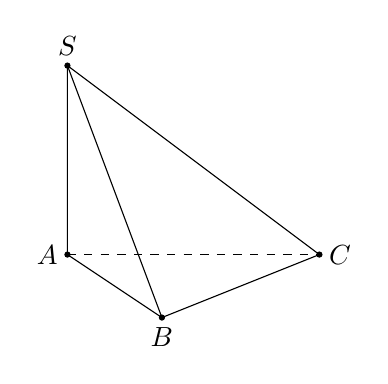
\begin{tikzpicture}[scale=0.8]
            \path (0,0) coordinate (A) -- (4,0) coordinate (C) -- (1.5,-1) coordinate (B) -- (0,3) coordinate (S);
            \draw (A) -- (B) -- (C) -- (S) -- (A) (S) node [above] {$S$} -- (B) node [below] {$B$};
            \draw [dashed] (A) node [left] {$A$} -- (C) node [right] {$C$};
            \foreach \x in {S,A,B,C} \draw [fill=black] (\x) circle (0.4 mm);
        \end{tikzpicture}
    }
    \loigiai{
        Vì $SA\perp (ABC)$ suy ra góc giữa đường thẳng $SC$ và mặt phẳng $(ABC)$ bằng $\widehat{SCA}$.\\
        Mà $\tan\widehat{SCA}=\dfrac{SA}{AC}=\dfrac{2a}{\sqrt{a^2+3a^2}}=1$.\\
        Vậy $\widehat{SCA}=45^{\circ}$
    }
\end{ex}
% Câu 14
\begin{ex}%[1H3B3-3]
    [THPT Phan Đình Phùng – Quảng Bình - 2021]
    \immini{
        Cho hình chóp $S.ABC$ có $SA$ vuông góc với mặt phẳng $(ABC)$, $SA=a\sqrt{2}$, tam giác $ABC$ vuông tại $A$ và $AC=a$, $\sin B=\dfrac{1}{\sqrt{3}}$ (minh hoạ như hình bên). Góc giữa đường thẳng $SB$ và mặt phẳng $(ABC)$ bằng
        \choice
        {$90^{\circ}$}
        {$30^{\circ}$}
        {\True $45^{\circ}$}
        {$60^{\circ}$}
    }{
        \begin{tikzpicture}[scale=1]
            \path (0,0) coordinate (A) -- (4,0) coordinate (C) -- (1.5,-1) coordinate (B) -- (0,3) coordinate (S);
            \draw (A) -- (B) -- (C) -- (S) -- (A) (S) node [above] {$S$} -- (B) node [below] {$B$};
            \draw [dashed] (A) node [left] {$A$} -- (C) node [right] {$C$};
            \foreach \x in {S,A,B,C} \draw [fill=black] (\x) circle (0.4 mm);
        \end{tikzpicture}
    }
    \loigiai{
        Ta có $SA\perp (ABC) \Rightarrow \left(\widehat{SB,(ABC)}\right)=\widehat{SBA}$.\\
        Do $\sin B=\sin \widehat{SBA}=\dfrac{1}{\sqrt{3}}$ nên ta có
        \[\Rightarrow \cos B=\cos \widehat{SBA}=\dfrac{\sqrt{6}}{3},\tan B=\tan \widehat{SBA}=\dfrac{AC}{AB}=\dfrac{1}{\sqrt{2}} \Rightarrow AB=a\sqrt{2}.\]
        Vậy tam giác $SAB$ vuông cân tại $A$.\\
        Suy ra $\left(\widehat{SB,(ABC)}\right)=\widehat{SBA}=45^{\circ}$.
    }
\end{ex}

\begin{ex}%[1H3B3-3]
    [THPT Hậu Lộc 4 - Thanh Hóa - 2021] Cho hình chóp $S.ABC$ có $SA\perp(ABC)$, $SA=a\sqrt{3}$, tam giác $ABC$ vuông tại $B$ có $AC=2a$, $BC=a$. Góc giữa đường thẳng $SB$ và mặt phẳng $(ABC)$ bằng
    \choice
    {$60^{\circ}$}
    {$90^{\circ}$}
    {$30^{\circ}$}
    {\True $45^{\circ}$}
    \loigiai{
        \immini{
            Vì $SA\perp(ABC)$ nên $AB$ là hình chiếu vuông góc của $SB$ lên $(ABC)$.\\
            Do đó $\left(\widehat{SB,(ABC)}\right)=\left(\widehat{SB,AB}\right)=\widehat{SBA}$.\\
            Tam giác $ABC$ vuông tại $B$ nên $AB=\sqrt{(2a)^2-a^2}=a\sqrt{3}$.\\
            Do đó $\triangle SAB$ vuông cân tại $A$ suy ra $\widehat{SBA}=45^{\circ}$.\\
            Vậy $\left(\widehat{SB,(ABC)}\right)=45^{\circ}$.}
        {
            \begin{tikzpicture}
                \def\a{4}
                \path 	(0:0) coordinate (A)
                ++(0:\a) coordinate (C)
                ++(-120:\a/2) coordinate (B)
                ($(A)+(90:\a)$) coordinate (S);
                \draw[dashed] 	(A)--(C);
                \draw (S)--(A)--(B) (B)--(C) (S)--(B) (S)--(C);
                \foreach \x/\g in {A/180,B/-90,C/0,S/90}
                \fill[black] 	(\x) circle (1pt)
                ($(\g:3mm)+(\x)$) node {$\x$};
                %Hình chóp S.ABC có SA vuông góc đáy
        \end{tikzpicture}}

    }
\end{ex}
\begin{ex}[Sở Lào Cai - 2021]%[1H3K3-3]%Câu 16.
    Cho hình lập phương $ABCD.A'B'C'D'$. Gọi $M$, $N$ lần lượt là trung điểm $AC$ và $B'C'$, $\alpha$ là góc giữa đường thẳng $MN$ và mặt phẳng $(A'B'C'D')$. Tính giá trị $\alpha$.
    \choice
    {$\sin\alpha=\dfrac{\sqrt{2}}{2}$}
    {\True $\sin\alpha=\dfrac{2\sqrt{5}}{5}$}
    {$\sin\alpha=\dfrac{1}{2}$}
    {$\sin\alpha=\dfrac{\sqrt{5}}{5}$}
    \loigiai{
        \begin{center}
            \begin{tikzpicture}[line cap=round,line join=round,>=triangle 45,thick]
                \draw (1,4)-- (4,4) -- (3,3) -- (0,3) -- (1,4);
                \draw [dashed] (0,0) -- (1,1) -- (1,4) (1,1) -- (4,1);
                \draw (0,0)-- (0,3) (3,3)-- (3,0) -- (0,0) (3,0)-- (4,1) -- (4,4) (1,4)-- (3,3);
                \draw [dashed] (2,3.5)-- (2,0.5) -- (3.5,0.5) -- (2,3.5);
                \draw (1,4) node[above] {$A$};
                \draw (4,4) node[above] {$B$};
                \draw (3,3) node[right] {$C$};
                \draw (0,3) node[left] {$D$};
                \draw (1,1) node[left] {$A'$};
                \draw (4,1) node[right] {$B'$};
                \draw (3,0) node [right] {$C'$};
                \draw (0,0) node [left] {$D'$};
                \draw (2,3.5) node[above] {$M$};
                \draw (3.5,0.5) node[right] {$N$};
                \draw (2,0.5) node[left] {$O'$};
            \end{tikzpicture}
        \end{center}
        Giả sử cạnh hình lập phương là $a$.\\
        Gọi $O'$ là tâm của hình vuông $A'B'C'D'$. Suy ra $O'N$ là hình chiếu của $MN$ lên $(A'B'C'D')$. Do đó góc giữa $MN$ và $(A'B'C'D')$ là góc giữa $MN$ và $O'N$.\\
        Tam giác $O'MN$ vuông tại $O$ có $O'N=\dfrac{1}{2}a$, $O'M=a$ nên\\ $\sin\widehat{O'NM}=\dfrac{O'M}{MN}=\dfrac{O'M}{\sqrt{O'N^2+O'M^2}}=\dfrac{a}{\sqrt{\dfrac{a^2}{4}+a^2}}=\dfrac{2\sqrt{5}}{5}$.
    }
\end{ex}
\begin{ex}[Sở Tuyên Quang - 2021]%[1H3K3-3]%Câu 17.
    Cho hình chóp $S.ABCD$ có đáy $ABCD$ là hình vuông cạnh $a$, đường thẳng $SA$ vuông góc với mặt phẳng đáy và $SA=2a$. Góc giữa đường thẳng $SC$ và mặt phẳng $(ABCD)$ là $\alpha$. Khi đó $\tan\alpha$ bằng
    \choice
    {$2\sqrt{2}$}
    {$2$}
    {\True $\sqrt{2}$}
    {$\dfrac{2}{\sqrt{3}}$}
    \loigiai{
        \begin{center}
            \begin{tikzpicture}[line cap=round,line join=round,>=triangle 45,thick]
                \draw (1,4) -- (4,) (1,4) -- (3,0) (1,4) -- (0,0);
                \draw [dashed] (0,0) -- (1,1) -- (1,4) (3,0) -- (1,1) -- (4,1);
                \draw (0,0)-- (3,0) -- (4,1);
                \draw [shift={(3,0)}] (0,0) -- (116.565:0.6) arc (116.565:153.435:0.6);
                \draw (1,4) node[above] {$S$};
                \draw (1,1) node[left] {$A$};
                \draw (4,1) node[right] {$B$};
                \draw (3,0) node [right] {$C$};
                \draw (0,0) node [left] {$D$};
                \draw (2.35,0.7) node {$\alpha$};
            \end{tikzpicture}
        \end{center}
        Ta có $\widehat{\left(SC;(ABCD)\right)}=\widehat{SCA}=\alpha$.\\
        Xét tam giác $SAC$ vuông tại $A$ có: $\tan\widehat{SCA}=\dfrac{SA}{AC} =\dfrac{2a}{a\sqrt{2}} =\sqrt{2}$ \\
        $ \Rightarrow\tan\alpha=\sqrt{2}$.
    }
\end{ex}
\begin{ex}[Chuyên Thoại Ngọc Hầu - An Giang - 2021]%[1H3K3-3]%Câu 18.
    Cho hình chóp $S.ABCD$ có đáy là hình vuông $ABCD$ cạnh bằng $3a$, $SA$ vuông góc với mặt đáy $(ABCD)$, $SB=5a$. Tính $\sin$ của góc giữa cạnh $SC$ và mặt đáy $(ABCD)$.
    \choice
    {$\dfrac{3\sqrt{2}}{4}$}
    {\True $\dfrac{2\sqrt{34}}{17}$}
    {$\dfrac{4}{5}$}
    {$\dfrac{2\sqrt{2}}{3}$}
    \loigiai{
        \begin{center}
            \begin{tikzpicture}[line cap=round,line join=round,>=triangle 45,thick]
                \draw (1,4) -- (4,) (1,4) -- (3,0) (1,4) -- (0,0);
                \draw [dashed] (0,0) -- (1,1) -- (1,4) (3,0) -- (1,1) -- (4,1);
                \draw (0,0)-- (3,0) -- (4,1);
                \draw [shift={(3,0)}] (0,0) -- (116.565:0.6) arc (116.565:153.435:0.6);
                \draw (1,4) node[above] {$S$};
                \draw (1,1) node[left] {$A$};
                \draw (4,1) node[right] {$B$};
                \draw (3,0) node [right] {$C$};
                \draw (0,0) node [left] {$D$};
                \draw (2.35,0.7) node {$\alpha$};
            \end{tikzpicture}
        \end{center}
        Do $SA\perp(ABCD)$ nên $AC$ là hình chiếu của $SC$ lên mặt phẳng $(ABCD)$. Do đó góc giữa cạnh $SC$ và mặt đáy $(ABCD)$ là $\widehat{SCA}$.\\
        Xét tam giác $ABC$ có $AC=\sqrt{AB^2+BC^2}=3a\sqrt{2}$.\\
        Xét tam giác $SAB$ có $SA=\sqrt{SB^2-AB^2}=4a$.\\
        Xét tam giác $SAC$ có $SC=\sqrt{SA^2+AC^2}=a\sqrt{34}$.\\
        Xét tam giác $SAC$ có $\sin\widehat{SCA}=\dfrac{SA}{SC}=\dfrac{4a}{a\sqrt{34}}=\dfrac{2\sqrt{34}}{17}$.\\
        Vậy $\sin$ của góc giữa cạnh $SC$ và mặt đáy $(ABCD)$ bằng $\dfrac{2\sqrt{34}}{17}$.
    }
\end{ex}
\begin{ex}[Chuyên Lê Hồng Phong - TPHCM - 2021]%[1H3K3-3]%Câu 19.
    Cho hình chóp $S.ABC$ có đáy $ABC$ là tam giác đều cạnh $a$, cạnh $SA$ vuông góc với mặt phẳng đáy và $SA=2a$, gọi $M$ là trung điểm của $SC$. Tính cosin của góc $\alpha$ là góc giữa đường thẳng $BM$ và $(ABC)$.
    \choice
    {$\cos\alpha=\dfrac{\sqrt{7}}{14}$}
    {$\cos\alpha=\dfrac{2\sqrt{7}}{7}$}
    {\True $\cos\alpha=\dfrac{\sqrt{21}}{7}$}
    {$\cos\alpha=\dfrac{\sqrt{5}}{7}$}
    \loigiai{
        \begin{center}
            \begin{tikzpicture}[line cap=round,line join=round,>=triangle 45,thick]
                \draw (1,4) -- (4,) (1,4) -- (3,0) (1,4) -- (0,0);
                \draw [dashed] (0,0) -- (1,1) -- (1,4) (3,0) -- (1,1) -- (4,1) -- (2,0.5) -- (2,2);
                \draw (0,0)-- (3,0) -- (4,1) -- (2,2);
                \draw [shift={(4,1)}] (0,0) -- (153.435:0.556) arc (153.435:194.036:0.556);
                \draw (1,4) node[above] {$S$};
                \draw (1,1.1) node[left] {$A$};
                \draw (4,1) node[right] {$B$};
                \draw (3,0) node [right] {$C$};
                \draw (0,0) node [left] {$D$};
                \draw (2,2) node [left] {$M$};
                \draw (2.1,0.6) node [below left] {$H$};
                \draw (3.2,1.2) node {$\alpha$};
            \end{tikzpicture}
        \end{center}
        Trong mặt phẳng $(SAC)$, dựng $MH\perp AC$ tại $H$.\\
        Do $SA\perp(ABC)\Rightarrow SA\perp AC\subset(ABC)\Rightarrow SA\parallel MH$.\\
        Khi đó: $MH\perp(ABC)$.\\
        Suy ra: $\left(\widehat{BM,(ABC)}\right)=\left(\widehat{BM,BH}\right)=\widehat{MBH}$. Khi đó:
        \[\cos\alpha=\dfrac{BH}{BM}=\dfrac{\dfrac{a\sqrt{3}}{2}}{\sqrt{\left(\dfrac{a\sqrt{3}}{2}\right)^2+\left(\dfrac{2a}{2}\right)^2}}=\dfrac{\sqrt{21}}{7}.\]
    }
\end{ex}
\begin{ex}[Chuyên Hoàng Văn Thụ - Hòa Bình - 2021]%[1H3B3-3]%Câu 20.
    Cho hình chóp $S.ABCD$ có đáy là hình vuông cạnh $a$, $SA\perp(ABC),SA=a\sqrt{2}$. Góc giữa đường thẳng $SC$ và mặt phẳng $(ABCD)$ bằng
    \choice
    {$60^{\circ}$}
    {$90^{\circ}$}
    {\True $45^{\circ}$}
    {$30^{\circ}$}
    \loigiai{
        \begin{center}
            \begin{tikzpicture}[line cap=round,line join=round,>=triangle 45,thick]
                \draw (1,4) -- (4,) (1,4) -- (3,0) (1,4) -- (0,0);
                \draw [dashed] (0,0) -- (1,1) -- (1,4) (3,0) -- (1,1) -- (4,1);
                \draw (0,0)-- (3,0) -- (4,1);
                \draw [shift={(3,0)}] (0,0) -- (116.565:0.6) arc (116.565:153.435:0.6);
                \draw (1,4) node[above] {$S$};
                \draw (1,1.1) node[left] {$A$};
                \draw (4,1) node[right] {$B$};
                \draw (3,0) node [right] {$C$};
                \draw (0,0) node [left] {$D$};
            \end{tikzpicture}
        \end{center}
        Ta có $AC=a\sqrt{2}$ suy ra $\triangle SAC$ vuông cân tại $A$.\\
        Góc giữa $SC$ và mp $(ABCD)$ chính là góc $\widehat{SCA}=45^{\circ}$.
    }
\end{ex}
\begin{ex}[Sở Yên Bái - 2021]%[1H3B3-3]%Câu 21.
    Cho hình chóp $S.ABCD$ có đáy là hình vuông canh $a, SA$ vuông góc với mặt phẳng đáy và $SA=a\sqrt{6}$. Góc giữa đường thẳng $SC$ và mặt phẳng $(ABCD)$ bằng
    \choice
    {\True $60^{\circ}$}
    {$45^{\circ}$}
    {$90^{\circ}$}
    {$30^{\circ}$}
    \loigiai{
        \begin{center}
            \begin{tikzpicture}[line cap=round,line join=round,>=triangle 45,thick]
                \draw (1,4) -- (4,) (1,4) -- (3,0) (1,4) -- (0,0);
                \draw [dashed] (0,0) -- (1,1) -- (1,4) (3,0) -- (1,1) -- (4,1);
                \draw (0,0)-- (3,0) -- (4,1);
                \draw [shift={(3,0)}] (0,0) -- (116.565:0.6) arc (116.565:153.435:0.6);
                \draw (1,4) node[above] {$S$};
                \draw (1,1.1) node[left] {$A$};
                \draw (4,1) node[right] {$B$};
                \draw (3,0) node [right] {$C$};
                \draw (0,0) node [left] {$D$};
            \end{tikzpicture}
        \end{center}
        Ta có $AC$ là hình chiếu của $SC$ lên mặt đáy $(ABCD)$ \\
        $\Rightarrow\widehat{\left(SC,(ABCD)\right)}=\widehat{(SC,AC)}=\widehat{SCA}\Rightarrow\tan\widehat{SCA}=\dfrac{SA}{AC}=\sqrt{3}\Rightarrow\widehat{\left(SC,(ABCD)\right)}=60^{\circ}$.
    }
\end{ex}
\begin{ex}[THPT Lương Thế Vinh - 2021]%[1H3K3-3]%Câu 22.
    Cho hình chóp $S.ABCD$ có đáy là hình thoi tâm $O$, $\triangle ABD$ đều cạnh $a\sqrt{2}, SA$ vuông góc với mặt phẳng đáy và $SA=\dfrac{3a\sqrt{2}}{2}$. Góc giữa đường thẳng $SO$ và mặt phẳng $(ABCD)$ bằng
    \choice
    {$45^{\circ}$}
    {$90^{\circ}$}
    {$30^{\circ}$}
    {\True $60^{\circ}$}
    \loigiai{
        \begin{center}
            \begin{tikzpicture}[line cap=round,line join=round,>=triangle 45,thick]
                \draw (1,4) -- (3,0) (4,1) -- (1,4) -- (0,0);
                \draw [dashed] (0,0) -- (1,1) -- (1,4) -- (2,0.5) (3,0) -- (1,1) -- (4,1);
                \draw (0,0)-- (3,0) -- (4,1);
                \draw [shift={(2,0.5)},dashed] (0,0) -- (105.945:0.452) arc (105.945:153.435:0.452) -- cycle;
                \draw (1,4) node[above] {$S$};
                \draw (1,1.1) node[left] {$A$};
                \draw (4,1) node[right] {$B$};
                \draw (3,0) node [right] {$C$};
                \draw (0,0) node [left] {$D$};
                \draw (2.1,0.4) node [left] {$O$};
            \end{tikzpicture}
        \end{center}
        Ta có: $ABCD$ là hình thoi có tâm là $O\Rightarrow O$ là trung điểm của $BD$.\\
        Mà $\triangle ABD$ đều nên $AO\perp BD$.\\
        Lại có $SA\perp(ABCD)\Rightarrow\widehat{\left(SO,(ABCD)\right)}=\widehat{SOA}$.\\
        Xét $\triangle ABO$ có: $AO=\sqrt{AB^2-BO^2}=\sqrt{(a\sqrt{2})^2-\left(\dfrac{a\sqrt{2}}{2}\right)^2}=\dfrac{a\sqrt{6}}{2}$.\\
        Ta có: $\tan\widehat{SAO}=\dfrac{SA}{AO}=\dfrac{\dfrac{3a\sqrt{2}}{2}}{\dfrac{a\sqrt{6}}{2}}=\sqrt{3}\Rightarrow\widehat{SOA}=60^{\circ}$.
    }
\end{ex}
\begin{ex}[THPT Đặng Thúc Hứa - Nghệ An - 2021]%[1H3B3-3]%Câu 23.
    Cho khối lăng trụ đứng $ABC.A'B'C'$ có $AA'=a\sqrt{6}$, đáy $ABC$ là tam giác vuông cân tại $B$ và $BA=BC=a$. Góc giữa đường thẳng $A'C$ và mặt phẳng đáy bằng
    \choice
    {$45^{\circ}$}
    {$90^{\circ}$}
    {\True $60^{\circ}$}
    {$30^{\circ}$}
    \loigiai{
        \begin{center}
            \begin{tikzpicture}[line cap=round,line join=round,>=triangle 45,thick]
                \draw (1,5)-- (4,5) -- (3,4) -- (1,1);
                \draw [dashed, thick] (1,1) -- (4,1);
                \draw (1,1)-- (3,0)-- (4,1) -- (4,5) (1,1) -- (1,5)-- (3,4) -- (3,0);
                \draw (1,5) node[above] {$A$};
                \draw (4,5) node[above] {$B$};
                \draw (3,4) node[right] {$C$};
                \draw (1,1) node[left] {$A'$};
                \draw (4,1) node[right] {$B'$};
                \draw (3,0) node [right] {$C'$};
            \end{tikzpicture}
        \end{center}
        Ta có $AA'\perp(ABC)\Rightarrow AC$ là hình chiếu của $A'C$ lên mặt phẳng $(ABC)$.\\
        Khi đó $\widehat{\left(A'C,(ABC)\right)}=\widehat{(A'C,AC)}=\widehat{A'CA}$.\\
        Ta có $AC=AB\sqrt{2}=a\sqrt{2}$.\\
        $\tan\widehat{A'CA}=\dfrac{AA'}{AC}=\dfrac{a\sqrt{6}}{a\sqrt{2}}=\sqrt{3}\Rightarrow\widehat{A'CA}=60^{\circ}$.
    }
\end{ex}
\begin{ex}[THPT Chu Văn An - Thái Nguyên - 2021]%[1H3B3-3]%Câu 24.
    Cho chóp $S.ABC$ có đáy là tam giác vuông tại $B$. $AB=3a,BC=\sqrt{3}a$. $SA$ vuông góc với đáy và $SA=2a$. Góc giữa $SC$ và đáy là
    \choice
    {$90^{\circ}$}
    {$45^{\circ}$}
    {$60^{\circ}$}
    {\True $30^{\circ}$}
    \loigiai{
        \begin{center}
            \begin{tikzpicture}[line cap=round,line join=round,>=triangle 45,thick]
                \draw (1,1) -- (1,4) -- (3,0) (4,1) -- (1,4);
                \draw [dashed] (1,1) -- (1,4) (3,0) -- (1,1) -- (4,1);
                \draw (1,1) -- (3,0) -- (4,1);
                \draw (1,4) node[above] {$S$};
                \draw (1,1.1) node[left] {$A$};
                \draw (4,1) node[right] {$C$};
                \draw (3,0) node [below] {$B$};
            \end{tikzpicture}
        \end{center}
        Ta có $AC=\sqrt{12}a$.\\
        Xét tam giác $\triangle SAC$ ta có  $\tan\widehat{SCA}=\dfrac{2a}{\sqrt{12}a}=\dfrac{1}{\sqrt{3}}\Rightarrow\widehat{SCA}={30}^{\circ}$.
    }
\end{ex}
\begin{ex}[THPT Quảng Xương 1-Thanh Hóa - 2021]%[1H3K3-3]%Câu 25.
    Cho hình chóp $S.ABCD$ có đáy là hình thoi tâm $O$, $\triangle ABD$ đều cạnh $a\sqrt{2}$, $SA$ vuông góc với mặt phẳng đáy và $SA=\dfrac{3a\sqrt{2}}{2}$. Góc giữa đường thẳng $SO$ và mặt phẳng $(ABCD)$ bằng
    \choice
    {$45^{\circ}$}
    {$30^{\circ}$}
    {\True $60^{\circ}$}
    {$90^{\circ}$}
    \loigiai{
        \begin{center}
            \begin{tikzpicture}[line cap=round,line join=round,>=triangle 45,thick]
                \draw (1,4) -- (3,0) (4,1) -- (1,4) -- (0,0);
                \draw [dashed] (0,0) -- (1,1) -- (1,4) -- (2,0.5) (3,0) -- (1,1) -- (4,1);
                \draw (0,0)-- (3,0) -- (4,1);
                \draw [shift={(2,0.5)},dashed] (0,0) -- (105.945:0.452) arc (105.945:153.435:0.452) -- cycle;
                \draw (1,4) node[above] {$S$};
                \draw (1,1.1) node[left] {$A$};
                \draw (4,1) node[right] {$B$};
                \draw (3,0) node [right] {$C$};
                \draw (0,0) node [left] {$D$};
                \draw (2.1,0.4) node [left] {$O$};
            \end{tikzpicture}
        \end{center}
        Tam giác $ABD$ đều cạnh $a\sqrt{2}$, suy ra $AO=\dfrac{(a\sqrt{2})\sqrt{3}}{2}=\dfrac{a\sqrt{6}}{2}$.\\
        Vì $SA\perp(ABCD)$, suy ra $OA$ là hình chiếu của $OS$ lên mặt phẳng $(ABCD)$, suy ra:\\
        $\left(SO;(ABCD)\right)=\widehat{SOA}$.\\
        Xét tam giác vuông $SAO$ ta có $\tan\widehat{SOA}=\dfrac{SA}{AO}=\dfrac{3a\sqrt{2}}{2}\cdot\dfrac{2}{a\sqrt{6}}=\sqrt{3}\Rightarrow\widehat{SOA}=60^{\circ}$.\\
        Vậy $\left(SO;(ABCD)\right)=60^{\circ}$.
    }
\end{ex}
\begin{ex}[Trung Tâm Thanh Tường - 2021]%[1H3B3-3]%Câu 26.
    Cho hình chóp $S.ABC$ có $SA\perp(ABC)$, $SA=a\sqrt{3}$, tam giác $ABC$ vuông tại $B$ có $AC=2a,BC=a\sqrt{3}$. Góc giữa $SB$ và mặt phẳng $(ABC)$ bằng
    \choice
    {$90^{\circ}$}
    {$45^{\circ}$}
    {$30^{\circ}$}
    {\True $60^{\circ}$}
    \loigiai{
        \begin{center}
            \begin{tikzpicture}[line cap=round,line join=round,>=triangle 45,thick]
                \draw (1,1) -- (1,4) -- (3,0) (4,1) -- (1,4);
                \draw [dashed] (1,1) -- (1,4) (3,0) -- (1,1) -- (4,1);
                \draw (1,1) -- (3,0) -- (4,1);
                \draw (1,4) node[above] {$S$};
                \draw (1,1.1) node[left] {$A$};
                \draw (4,1) node[right] {$C$};
                \draw (3,0) node [below] {$B$};
            \end{tikzpicture}
        \end{center}
        Ta có $AB=\sqrt{AC^2-BC^2}=\sqrt{(2a)^2-(a\sqrt{3})^2}=a$.\\
        Dễ thấy $\widehat{\left(SB;(ABC)\right)}=\widehat{(SB;AB)}=\widehat{SBA}$. Khi đó $\tan\widehat{SBA}=\dfrac{SA}{AB}=\dfrac{a\sqrt{3}}{a}=\sqrt{3}\Rightarrow\widehat{SBA}=60^{\circ}$.\\
        Vậy $\widehat{\left(SB;(ABC)\right)}=60^{\circ}$.
    }
\end{ex}
\begin{ex}[THPT Trần Phú - Đà Nẵng - 2021]%[1H3K3-3]%Câu 27.
    \immini{
        Cho hình chóp tứ giác $S.ABCD$ có đáy $ABCD$ là hình vuông tâm $I$, cạnh $a$. Biết $SA$ vuông góc với mặt đáy $(ABCD)$ và $SA=a\sqrt{3}$ (tham khảo hình vẽ bên). Khi đó $\tan$ của góc giữa đường thẳng $SI$ và mặt phẳng $(ABCD)$ là
        \choice
        {\True $\sqrt{6}$}
        {$\dfrac{\sqrt{6}}{6}$}
        {$\sqrt{3}$}
        {$\dfrac{\sqrt{3}}{3}$}
    }{
        \begin{tikzpicture}[line cap=round,line join=round,>=triangle 45,thick]
            \draw (1,4) -- (3,0) (4,1) -- (1,4) -- (0,0);
            \draw [dashed] (0,0) -- (1,1) -- (1,4) -- (2,0.5) (3,0) -- (1,1) -- (4,1) -- (0,0);
            \draw (0,0)-- (3,0) -- (4,1);
            \draw (1,4) node[above] {$S$};
            \draw (1,1.1) node[left] {$A$};
            \draw (4,1) node[right] {$B$};
            \draw (3,0) node [right] {$C$};
            \draw (0,0) node [left] {$D$};
            \draw (2.25,0.25) node [left] {$I$};
        \end{tikzpicture}
    }
    \loigiai{
        Ta có: $AI=\dfrac{1}{2}AC=\dfrac{a\sqrt{2}}{2}$.\\
        Mà $SA\perp(ABCD)$ nên $AI$ là hình chiếu của $SI$ trên mặt phẳng $(ABCD)$ \\
        $ \Rightarrow\widehat{\left(SI;(ABCD)\right)}=\widehat{(SI; AI)}=\widehat{SIA} $ (do tam giác $SAI$ vuông tại $A$).\\
        Vậy $\tan\widehat{\left(SI;(ABCD)\right)}=\tan\widehat{SIA}=\dfrac{SA}{AI}=\sqrt{6}$.
    }
\end{ex}
\begin{ex}[Chuyên Biên Hòa - 2021]%[1H3K3-3]%Câu 28.
    Cho hình chóp $S.ABCD$ có đáy $ABCD$ là hình thoi cạnh $a$, $O$ là giao điểm của $AC$ và $BD$. $\widehat{ABC}=60^{\circ}$; $SO$ vuông góc với $(ABCD)$ và $SO=a\sqrt{3}$. Góc giữa $SB$ và mặt phẳng $(SAC)$ bằng
    \choice
    {\True $\left(25^{\circ}; 27^{\circ}\right)$}
    {$\left(62^{\circ}; 66^{\circ}\right)$}
    {$\left(53^{\circ}; 61^{\circ}\right)$}
    {$\left(27^{\circ}; 33^{\circ}\right)$}
    \loigiai{
        \begin{center}
            \begin{tikzpicture}[line cap=round,line join=round,>=triangle 45,thick]
                \draw (2,4) -- (3,0) (4,1) -- (2,4) -- (0,0);
                \draw [dashed] (0,0) -- (1,1) -- (2,4) -- (2,0.5) (3,0) -- (1,1) -- (4,1) (0,0) -- (4,1);
                \draw (0,0)-- (3,0) -- (4,1);
                \draw (2,4) node[above] {$S$};
                \draw (1,1.1) node[left] {$A$};
                \draw (4,1) node[right] {$B$};
                \draw (3,0) node [right] {$C$};
                \draw (0,0) node [left] {$D$};
                \draw (2.25,0.25) node [left] {$O$};
            \end{tikzpicture}
        \end{center}
        Ta có $\widehat{ABC}=60^{\circ};\triangle ABC$ cân tại $B$ nên $\triangle ABC$ đều cạnh $a$.\\
        Suy ra: $BO=\dfrac{a\sqrt{3}}{2}$.\\
        Do $OB\perp (SAC)$ nên góc giữa $SB$ và mặt phẳng $(SAC)$ chính là góc $\widehat{BSO}$.\\
        Ta có tam giác $SOB$ vuông tại $O$ nên $\tan\widehat{BSO}=\dfrac{BO}{SO}=\dfrac{1}{2}\Rightarrow\widehat{BSO}\approx 26,56^{\circ}$.
    }
\end{ex}
\begin{ex}[Sở Cần Thơ - 2021]%[1H3B3-3]%Câu 29
    Cho hình chóp $S.ABC$ có tam giác $ABC$ vuông tại $B$, có $AB=a\sqrt{3}$, $BC=a, SA$ vuông góc với mặt phẳng $(ABC)$ và $SA=2a$. Góc giữa đường thẳng $SC$ và mặt phẳng $(ABC)$ bằng
    \choice
    {\True $45^{\circ}$}
    {$30^{\circ}$}
    {$60^{\circ}$}
    {$90^{\circ}$}
    \loigiai{
        \begin{center}
            \begin{tikzpicture}[line cap=round,line join=round,>=triangle 45,thick]
                \draw (1,1) -- (1,4) -- (3,0) (4,1) -- (1,4);
                \draw [dashed] (1,1) -- (1,4) (3,0) -- (1,1) -- (4,1);
                \draw (1,1) -- (3,0) -- (4,1);
                \draw (1,4) node[above] {$S$};
                \draw (1,1.1) node[left] {$A$};
                \draw (4,1) node[right] {$C$};
                \draw (3,0) node [below] {$B$};
            \end{tikzpicture}
        \end{center}
        Hình chiếu của $SC$ lên mặt phẳng $(ABC)$ là $AC$. Khi đó $(SC,(ABC))=(SC, AC)=\widehat{SCA}$.\\
        Xét tam giác $ABC$ vuông tại $B$ ta có $AC=\sqrt{AB^2+BC^2}=\sqrt{(a\sqrt{3})^2+a^2}=2a$.\\
        Xét tam giác $SAC$ vuông tại $A$ ta có $\tan\widehat{SCA}=\dfrac{SA}{AC}=\dfrac{2a}{2a}=1\Rightarrow\widehat{SCA}=45^{\circ}$.
    }
\end{ex}
\begin{ex}[Sở Quảng Bình - 2021]%[1H3B3-3]
    Cho hình chóp $S.ABCD$ có đáy $ABCD$ là hình vuông cạnh $a$, biết $SA\perp(ABCD)$ và $SA=a\sqrt{2}$. Góc giữa đường thẳng $SC$ và mặt phẳng $(ABCD)$ bằng
    \choice
    {$60^{\circ}$}
    {\True $45^{\circ}$}
    {$30^{\circ}$}
    {$90^{\circ}$}
    \loigiai{\immini{
            Ta có $SA\perp(ABCD)$ nên $AC$ là hình chiếu của $SC$ trên mặt phẳng $(ABCD)$.\\
            Do đó: $\widehat{\left(SC,(ABCD)\right)}=\widehat{(SC,AC)}=\widehat{SCA}$.\\
            Xét hình vuông $ABCD$ ta có: $AC=a\sqrt{2}$.\\
            Xét $\triangle ABC$ vuông tại $A$, ta có: $\tan \widehat{SCA}=\dfrac{SA}{AC}=\dfrac{a\sqrt{2}}{a\sqrt{2}}=1\Rightarrow\widehat{SCA}=45^{\circ}$.	}
        {	\begin{tikzpicture}[scale=0.57,>=stealth, font=\footnotesize, line join=round, line cap=round]	%hình chóp có đáy là hình thang.
                \coordinate[label=above left:$A$] (A) at (0,0);
                \coordinate[label=below left:$B$] (B) at (-4,-3);
                \coordinate[label=below left:$C$] (C) at (4,-3);
                \coordinate[label=right:$D$] (D) at (8,0);
                \coordinate[label=above:$S$] (S) at ($(A)+(0,6)$);
                \draw (S)--(B)--(C)--(D)--(S)--(C);
                \draw[dashed] (A)--(B) (S)--(A)--(D) (A)--(C);
                \pic[draw,angle radius=2mm,angle eccentricity=2] {right angle = S--A--D};
                \pic[draw,angle radius=4mm,angle eccentricity=2] {angle = S--C--A};
                \foreach \diem in {A,B,C,D,S}	\fill (\diem)circle(1.5pt);
        \end{tikzpicture}}
    }
\end{ex}
\begin{ex}[Chuyên Tuyên Quang - 2021]%[1H3B3-3]
    Cho hình chóp $S.ABCD$ có đáy là hình thoi tâm $O$, tam giác $ABD$ đều cạnh bằng $a\sqrt{2}$, $SA=\dfrac{3a\sqrt{2}}{2}$ và vuông góc với mặt phẳng đáy. Góc giữa đường thẳng $SO$ và mặt phẳng $(ABCD)$ bằng
    \choice
    {\True $60^{\circ}$}
    {$45^{\circ}$}
    {$30^{\circ}$}
    {$90^{\circ}$}
    \loigiai{\immini{
            Ta có $AO$ là hình chiếu vuông góc của $SO$ trên mp $(ABCD)$ nên góc giữa giữa đường thẳng $SO$ và mặt phẳng $(ABCD)$ bằng góc giữa $SO$ và $AO$.\\
            Xét tam giác $SAO$ vuông tại $A$ có\\ $SA=\dfrac{3a\sqrt{2}}{2}$; $AO=\dfrac{a\sqrt{6}}{2}$.\\
            $\tan\widehat{SOA}=\dfrac{SA}{OA}=\dfrac{\dfrac{3a\sqrt{2}}{2}}{\dfrac{\sqrt{6}a}{2}}=\sqrt{3}\Rightarrow\widehat{SOA}=60^{\circ}$.\\
            Vậy góc giữa giữa đường thẳng $SO$ và mặt phẳng $(ABCD)$ bằng $60^{\circ}$.}
        {\begin{tikzpicture}[scale=0.57,>=stealth, font=\footnotesize, line join=round, line cap=round]	%hình chóp có đáy là hình thang.
                \coordinate[label=above left:$A$] (A) at (0,0);
                \coordinate[label=below left:$B$] (B) at (-4,-3);
                \coordinate[label=below left:$C$] (C) at (4,-3);
                \coordinate[label=right:$D$] (D) at (8,0);
                \coordinate[label=above:$S$] (S) at ($(A)+(0,4)$);
                \coordinate[label=below:$O$] (O) at ($(B)!1/2!(D)$);
                \draw (S)--(B)--(C)--(D)--(S)--(C);
                \draw[dashed] (C)--(A)--(B) (S)--(A)--(D) (B)--(D) (S)--(O);
                \pic[draw,angle radius=2mm,angle eccentricity=2] {right angle = S--A--B};
                \pic[draw,angle radius=2mm,angle eccentricity=2] {right angle = S--A--D};
                \pic[draw,angle radius=4mm,angle eccentricity=2] {angle = S--O--A};
                \foreach \diem in {A,B,C,D,S,O}	\fill (\diem)circle(1.5pt);
        \end{tikzpicture}}
    }
\end{ex}
\begin{ex}[Chuyên Vinh - 2021]%[1H3K3-3]
    Cho hình lăng trụ tam giác đều $ABC.A'B'C'$ có $AB=a$, $AA'=a\sqrt{2}$. Góc giữa đường thẳng $A'C$ và mặt phẳng $(ABB'A')$ bằng
    \choice
    {$45^{\circ}$}
    {$75^{\circ}$}
    {$60^{\circ}$}
    {\True $30^{\circ}$}
    \loigiai{
        \immini{
            Gọi $M$ là trung điểm $AB$. Do tam giác $ABC$ đều nên $CM\perp AB$.\\
            Lại có $CM\perp A'A$ nên suy ra $CM\perp(ABB'A')\\ \Rightarrow\widehat{\left(A'C,(ABB'A')\right)}=\widehat{(A'C, A'M)}=\widehat{MA'C}$.\\
            Ta có $A'C=\sqrt{A'A^2+AC^2}=\sqrt{2a^2+a^2}=a\sqrt{3}$ và $CM=\dfrac{a\sqrt{3}}{2}$.\\
            Trong tam giác vuông $CMA'$, ta có\\ $\sin\widehat{MA'C}=\dfrac{MC}{A'C}=\dfrac{\dfrac{a\sqrt{3}}{2}}{a\sqrt{3}}=\dfrac{1}{2}\Rightarrow\widehat{MA'C}=30^{\circ}$.\\
            Vậy góc giữa đường thẳng $A'C$ và mặt phẳng $(ABB'A')$ bằng $30^{\circ}$.	}
        {\begin{tikzpicture}[scale=0.7, font=\footnotesize, line join=round, line cap=round, >=stealth]
                \coordinate[label=above :$A'$] (A') at (0,4);
                \coordinate[label=above:$B'$] (B') at (4.5,2.5);
                \coordinate[label=right :$C'$] (C') at (6,4);
                \coordinate[label=below :$A$] (A) at (0,0);
                \coordinate[label=below :$B$] (B) at ($(A)+(B')-(A')$);
                \coordinate[label=below :$C$] (C) at ($(B)+(C')-(B')$);
                \coordinate[label=below :$M$] (M) at ($(A)!0.5!(B)$);
                \draw (A)--(B)--(C)--(C')--(A')--(B')--(B) (B')--(C') (A)--(A')--(B);
                \draw[dashed] (A)--(C) (A')--(M)--(C) (A')--(C);
                \pic[draw,angle radius=2mm,angle eccentricity=1.5] {right angle = C--M--B};
                \pic[draw,angle radius=4mm,angle eccentricity=2] {angle = M--A'--C};
                \foreach \diem in {A,B,M,A',B',C'}	\fill (\diem)circle(1.5pt);
        \end{tikzpicture}}
    }
\end{ex}
\begin{ex}[Cụm Liên Trường Hải Phòng 2019]%[1H3K3-3]
    Cho khối chóp $S.ABC$ có $SA\perp(ABC)$, tam giác $ABC$ vuông tại $B$, $AC=2a$, $BC=a$, $SB=2a\sqrt{3}$. Tính góc giữa $SA$ và mặt phẳng $(SBC)$.
    \choice
    {$45^{\circ}$}
    {\True $30^{\circ}$}
    {$60^{\circ}$}
    {$90^{\circ}$}
    \loigiai{
        \immini{
            Trong $(SAB)$ kẻ $AH\perp SB (H\in SB)$.\\
            Vì $\heva{&SA\perp BC\\&AB\perp BC}\Rightarrow BC\perp(SAB)\Rightarrow BC\perp AH$.\\
            Mà $SB\perp AH$ do cách dựng nên $AH\perp(SBC)$, hay $H$ là hình chiếu của $A$ lên $(SBC)$ suy ra góc giữa $SA$ và $(SBC)$ là góc $\widehat{ASH}$ hay góc $\widehat{ASB}$.\\
            Tam giác $ABC$ vuông ở $B\Rightarrow AB=\sqrt{AC^2-BC^2}=a\sqrt{3}$.\\
            Tam giác $SAB$ vuông ở $A\Rightarrow\sin\widehat{ASB}=\dfrac{AB}{SB}=\dfrac{1}{2}\Rightarrow\widehat{ASB}=30^{\circ}$.}
        {\begin{tikzpicture}[scale=0.8,>=stealth, font=\footnotesize, line join=round, line cap=round]
                \coordinate (S) at (0,3);
                \coordinate (A) at (0,0);
                \coordinate (B) at (2.5,-1.5);
                \coordinate (C) at (5,0);
                \coordinate[label=below:$H$] (H) at ($(S)!0.75!(B)$);
                \draw (A) node[left]{$A$}--(B) node[below]{$B$}--(C) node[right]{$C$}--(S) node[above]{$S$}--(A)--(H) (S)--(B);
                \draw[dashed] (A)--(C);
                \pic[draw,angle radius=2mm,angle eccentricity=2] {right angle = S--A--C};
                \pic[draw,angle radius=2mm,angle eccentricity=2] {right angle = S--H--A};
                \pic[draw,angle radius=4mm,angle eccentricity=2] {right angle =A--B--C};
                \pic[draw,angle radius=4mm,angle eccentricity=4] {angle = A--S--B};
                \foreach \diem in {A,B,C,H}	\fill (\diem)circle(1.5pt);
            \end{tikzpicture}
        }
    }
\end{ex}
\begin{ex}[Chuyên Bắc Ninh 2019]%[1H3K3-3]
    Cho hình chóp $SABCD$ có đáy là hình thang vuông tại $A$ và $B$,  $AB=BC=a,AD=2a$. Biết $SA$ vuông góc với đáy $(ABCD)$ và $SA=a$. Gọi $M$, $N$ lần lượt là trung điểm của $SB$ và $CD$. Tính sin góc giữa đường thẳng $MN$ và mặt phẳng $\left(SAC\right)$.
    \choice
    {$\dfrac{\sqrt{5}}{5}$}
    {$\dfrac{\sqrt{55}}{10}$}
    {\True $\dfrac{3\sqrt{5}}{10}$}
    {$\dfrac{2\sqrt{5}}{5}$}
    \loigiai{
        \immini{	Ta gọi $E,~F$ lần lượt là trung điểm của $SC,~AB$.\\
            Ta có $ME\parallel NF$ (do cùng song song với $BC$).\\ Nên tứ giác $MENF$ là hình thang,\\
            và $\heva{&MF\parallel SA\\&SA\perp (ABCD)}\Rightarrow MF\perp (ABCD)$\\ hay tứ giác $MENF$ là hình thang vuông tại $M,~F$.\\
            Gọi $K=NF\cap AC,I=EK\cap M$ thì $I=MN\cap (SAC)$.\\
            Ta có $\heva{&NC\perp AC\\&NC\perp SA}\Rightarrow NC\perp (SAC)$\\ hay $C$ là hình chiếu vuông góc của $N$ lên $(SAC)$.\\
            Từ đó ta có được, góc giữa $MN$ và $(SAC)$ là góc giữa $MN$ và $CI$.\\
            Suy ra, gọi $\alpha$ là góc giữa $MN$ và $(SAC)$ thì $\sin\alpha=\dfrac{CN}{IN}$.
        }
        {\begin{tikzpicture}[scale=0.8,>=stealth, font=\footnotesize, line join=round, line cap=round]	%hình chóp có đáy là hình thang.
                \coordinate[label=left:$A$] (A) at (0,0);
                \coordinate[label=below left:$B$] (B) at (-2,-3);
                \coordinate[label=below left:$C$] (C) at (1,-3);
                \coordinate[label=right:$D$] (D) at (6,0);
                \coordinate[label=above:$S$] (S) at ($(A)+(0.5,4)$);
                \coordinate[label=below:$N$] (N) at ($(C)!.5!(D)$);
                \coordinate[label= left:$M$] (M) at ($(S)!.5!(B)$);
                \coordinate[label= below right:$F$] (F) at ($(A)!.5!(B)$);
                \coordinate[label=right:$E$] (E) at ($(S)!0.5!(C)$);
                \coordinate[label=below left:$K$] (K) at (intersection of N--F and A--C);
                \coordinate[label=below left:$I$] (I) at (intersection of E--K and M--N);
                \draw (S)--(B)--(C)--(D)--(S)--(C) (M)--(E)--(N);
                \draw[dashed] (C)--(A)--(B) (S)--(A)--(D) (F)--(A) (C)--(I) (F)--(N) (M)--(F) (K)--(E) (M)--(N);
                \pic[draw,angle radius=2mm,angle eccentricity=2] {right angle = B--F--A};
                \pic[draw,angle radius=2mm,angle eccentricity=2] {right angle = B--A--D};
                \pic[draw,angle radius=2mm,angle eccentricity=2] {right angle = C--B--A};
                \pic[draw,angle radius=2mm,angle eccentricity=2] {right angle = A--C--D};
                \pic[draw,angle radius=2mm,angle eccentricity=2] {right angle = S--A--D};
                \pic[draw,angle radius=2mm,angle eccentricity=2] {right angle = E--M--F};
                \pic[draw,angle radius=2mm,angle eccentricity=2] {right angle = M--F--N};
                \pic[draw,angle radius=8mm,angle eccentricity=2] {angle = S--C--A};
                \foreach \diem in {A,B,C,D,S,M,N,K,F,I,E}	\fill (\diem)circle(1.5pt);
        \end{tikzpicture}}
        \noindent
        $NC=\dfrac{1}{2}CD=\dfrac{a\sqrt{2}}{2}$; $\dfrac{IN}{IM}=\dfrac{KN}{ME}=2\Rightarrow IN=\dfrac{2}{3}MN =\dfrac{2}{3}\sqrt{MF^2+FN^2}=\dfrac{a\sqrt{10}}{3}$.\\
        Vậy $\sin\alpha=\dfrac{CN}{IN}=\dfrac{3\sqrt{5}}{10}$.
    }
\end{ex}
\begin{ex}[Mã 102 - 2018]%[1H3B3-3]
    Cho hình chóp $S.ABCD$ có đáy là hình vuông cạnh $a$, $SA$ vuông góc với mặt phẳng đáy và $SA=\sqrt{6}a$. Góc giữa đường thẳng $SC$ và mặt phẳng đáy bằng
    \choice
    {$45^{\circ}$}
    {\True $60^{\circ}$}
    {$30^{\circ}$}
    {$90^{\circ}$}
    \loigiai{\immini
        {
            Do $SA\perp(ABCD)$ nên góc giữa đường thẳng $SC$ và mặt phẳng đáy bằng góc $\widehat{SCA}$.\\
            Ta có $SA=\sqrt{6}a$, $AC=\sqrt{2}a\\ \Rightarrow\tan\widehat{SCA}=\dfrac{SA}{AC} =\sqrt{3}\Rightarrow\widehat{SCA}=60^{\circ}$.\\
            Vậy góc giữa đường thẳng $SC$ và và mặt phẳng đáy bằng bằng $60^{\circ}$.}
        {	\begin{tikzpicture}[scale=0.5,>=stealth, font=\footnotesize, line join=round, line cap=round]
                \coordinate[label=above left:$A$] (A) at (0,0);
                \coordinate[label=below left:$B$] (B) at (-4,-3);
                \coordinate[label=below left:$C$] (C) at (4,-3);
                \coordinate[label=right:$D$] (D) at (8,0);
                \coordinate[label=above:$S$] (S) at ($(A)+(0,6)$);
                \draw (S)--(B)--(C)--(D)--(S)--(C);
                \draw[dashed] (A)--(B) (S)--(A)--(D) (A)--(C);
                \pic[draw,angle radius=2mm,angle eccentricity=2] {right angle = S--A--D};
                \pic[draw,angle radius=4mm,angle eccentricity=2] {angle = S--C--A};
                \foreach \diem in {A,B,C,D,S}	\fill (\diem)circle(1.5pt);
        \end{tikzpicture}}
    }
\end{ex}
\begin{ex}[Mã 101 - 2018]%[1H3B3-3]
    Cho hình chóp $S.ABCD$ có đáy là hình vuông cạnh $a$, $SA$ vuông góc với mặt phẳng đáy và $SB=2a$. Góc giữa đường thẳng $SB$ và mặt phẳng đáy bằng
    \choice
    {$45^{\circ}$}
    {\True $60^{\circ}$}
    {$90^{\circ}$}
    {$30^{\circ}$}
    \loigiai{
        \immini{Do $SA\perp(ABCD)$ nên góc giữa đường thẳng $SB$ và mặt phẳng đáy bằng góc $\widehat{SBA}$.\\
            Ta có $\cos\widehat{SBA}=\dfrac{AB}{SB} =\dfrac{1}{2}\Rightarrow\widehat{SBA}=60^{\circ}$.\\
            Vậy góc giữa đường thẳng $SB$ và và mặt phẳng đáy bằng bằng $60^{\circ}$.	}
        {	\begin{tikzpicture}[scale=0.5,>=stealth, font=\footnotesize, line join=round, line cap=round]
                \coordinate[label=above left:$A$] (A) at (0,0);
                \coordinate[label=below left:$B$] (B) at (-4,-3);
                \coordinate[label=below left:$C$] (C) at (4,-3);
                \coordinate[label=right:$D$] (D) at (8,0);
                \coordinate[label=above:$S$] (S) at ($(A)+(0,6)$);
                \draw (S)--(B)--(C)--(D)--(S)--(C);
                \draw[dashed] (A)--(B) (S)--(A)--(D);
                \pic[draw,angle radius=2mm,angle eccentricity=2] {right angle = S--A--D};
                \pic[draw,angle radius=4mm,angle eccentricity=2] {angle = A--B--S};
                \foreach \diem in {A,B,C,D,S}	\fill (\diem)circle(1.5pt);
    \end{tikzpicture}}	}
\end{ex}
\begin{ex}[Mã 101 - 2019]%[1H3B3-3]
    \immini{	Cho hình chóp $S.ABC$ có $SA$ vuông góc với mặt phẳng $(ABC)$,     $SA=2a$, tam giác $ABC$ vuông tại $B, AB=a\sqrt{3}$ và $BC=a$ (minh họa như hình vẽ bên). Góc giữa đường thẳng $SC$ và mặt phẳng $(ABC)$ bằng
        \choice
        {\True $45^{\circ}$}
        {$30^{\circ}$}
        {$60^{\circ}$}
        {$90^{\circ}$}}
    {	{\begin{tikzpicture}[scale=0.8,>=stealth, font=\footnotesize, line join=round, line cap=round]
                \coordinate (S) at (0,3);
                \coordinate (A) at (0,0);
                \coordinate (B) at (2.5,-1.5);
                \coordinate (C) at (5,0);
                \draw (A) node[left]{$A$}--(B) node[below]{$B$}--(C) node[right]{$C$}--(S) node[above]{$S$}--(A) (S)--(B);
                \draw[dashed] (A)--(C);
                \pic[draw,angle radius=2mm,angle eccentricity=2] {right angle = S--A--C};
                \pic[draw,angle radius=4mm,angle eccentricity=2] {right angle =A--B--C};
                \pic[draw,angle radius=4mm,angle eccentricity=4] {angle = S--C--A};
                \foreach \diem in {A,B,C,S}	\fill (\diem)circle(1.5pt);
            \end{tikzpicture}
    }}
    \loigiai{
        Ta có $SA\perp (ABC)$ nên $AC$ là hình chiếu của $SC$ lên mặt phẳng $(ABC)$.\\
        Do đó $\left(SC,(ABC)\right)=(SC,AC)=\widehat{SCA}$.\\
        Tam giác $ABC$ vuông tại $B, AB=a\sqrt{3}$ và $BC=a$ nên $AC=\sqrt{AB^2+BC^2}=\sqrt{4a^2}=2a$.\\
        Do đó tam giác $SAC$ vuông cân tại $A$ nên $\widehat{SCA}=45^{\circ}$.\\
        Vậy $\left(SC,(ABC)\right)=45^{\circ}$.
    }
\end{ex}
\begin{ex}[Đề Tham Khảo 2018]%[1H3K3-3]
    \immini{
        Cho hình chóp tứ giác đều $S.ABCD$ có tất cả các cạnh bằng $a$. Gọi $M$ là trung điểm của $SD$ (tham khảo hình vẽ bên). Tang của góc giữa đường thẳng $BM$ và mặt phẳng $(ABCD)$ bằng
        \choice
        {$\dfrac{\sqrt{2}}{2}$}
        {$\dfrac{\sqrt{3}}{3}$}
        {$\dfrac{2}{3}$}
        {\True $\dfrac{1}{3}$}
    }
    {\begin{tikzpicture}[scale=1,>=stealth, font=\footnotesize, line join=round, line cap=round]
            \coordinate[label=left:$A$] (A) at (0,0);
            \coordinate[label=below:$B$] (B) at (-1.9,-1.6);
            \coordinate[label=below:$C$] (C) at (1.6,-1.6);
            \coordinate[label=right:$D$] (D) at ($(A)+(C)-(B)$);
            \coordinate[label=above:$S$] (S) at ($(O)+(0,3.5)$);
            \coordinate[label=right:$M$] (M) at ($(S)!0.5!(D)$);
            \draw (S)--(B)--(C)--(D)--(S)--(C);
            \draw[dashed] (D)--(A) (S)--(A)--(B)--(M);
            \foreach \diem in {A,B,C,S,M}	\fill (\diem)circle(1.5pt);
    \end{tikzpicture}}
    \loigiai{
        \immini{
            Gọi $O$ là tâm của hình vuông.\\ Ta có $SO\perp(ABCD)$ và $SO=\sqrt{a^2-\dfrac{a^2}{2}}=\dfrac{a\sqrt{2}}{2}$.\\
            Gọi $M$ là trung điểm của $OD$ ta có $MH\parallel SO$ nên $H$ là hình chiếu của $M$ lên mặt phẳng $(ABCD)$ và $MH=\dfrac{1}{2}SO=\dfrac{a\sqrt{2}}{4}$.\\
            Do đó góc giữa đường thẳng $BM$ và mặt phẳng $(ABCD)$ là $\widehat{MBH}$.\\
            Khi đó ta có $\tan\widehat{MBH}=\dfrac{MH}{BH}=\dfrac{\dfrac{a\sqrt{2}}{4}}{\dfrac{3a\sqrt{2}}{4}}=\dfrac{1}{3}$.
        }
        {\begin{tikzpicture}[scale=1,>=stealth, font=\footnotesize, line join=round, line cap=round]
                \coordinate[label=left:$A$] (A) at (0,0);
                \coordinate[label=below:$B$] (B) at (-1.9,-1.6);
                \coordinate[label=below:$C$] (C) at (1.6,-1.6);
                \coordinate[label=right:$D$] (D) at ($(A)+(C)-(B)$);
                \coordinate[label=below:$O$] (O) at ($(A)!1/2!(C)$);
                \coordinate[label=above:$S$] (S) at ($(O)+(0,3.5)$);
                \coordinate[label=right:$M$] (M) at ($(S)!0.5!(D)$);
                \coordinate[label=below:$H$] (H) at ($(O)!0.5!(D)$);
                \draw (S)--(B)--(C)--(D)--(S)--(C);
                \draw[dashed](S)--(O) (D)--(A)--(C) (B)--(D) (S)--(A)--(B)--(M)--(H);
                \pic[draw,angle radius=4mm,angle eccentricity=2] {right angle =S--O--D};
                \pic[draw,angle radius=4mm,angle eccentricity=2] {right angle =M--H--D};
                \pic[draw,angle radius=4mm,angle eccentricity=2] {angle = H--B--M};
                \foreach \diem in {A,B,C,S,M,O,H}	\fill (\diem)circle(1.5pt);
        \end{tikzpicture}}
        Vậy tang của góc giữa đường thẳng $BM$ và mặt phẳng $(ABCD)$ bằng $\dfrac{1}{3}$.
    }
\end{ex}
\begin{ex}[Mã 104 - 2019]%[1H3K3-3]
    \immini{
        Cho hình chóp $S.ABC$ có $SA$ vuông góc với mặt phẳng $(ABC)$, $SA=2a$, tam giác $ABC$ vuông cân tại $B$ và $AB=a\sqrt{2}$ (minh họa như hình vẽ bên). Góc giữa đường thẳng $SC$ và mặt phẳng $(ABC)$ bằng
        \choice
        {$30^{\circ}$}
        {$90^{\circ}$}
        {$60^{\circ}$}
        {\True $45^{\circ}$}
    }
    {\begin{tikzpicture}[scale=0.8,>=stealth, font=\footnotesize, line join=round, line cap=round]
            \coordinate (S) at (0,3);
            \coordinate (A) at (0,0);
            \coordinate (B) at (2.5,-1.5);
            \coordinate (C) at (5,0);
            \draw (A) node[left]{$A$}--(B) node[below]{$B$}--(C) node[right]{$C$}--(S) node[above]{$S$}--(A) (S)--(B);
            \draw[dashed] (A)--(C);
            \pic[draw,angle radius=2mm,angle eccentricity=2] {right angle = S--A--C};
            \pic[draw,angle radius=4mm,angle eccentricity=2] {right angle =A--B--C};
            \pic[draw,angle radius=4mm,angle eccentricity=4] {angle = S--C--A};
            \foreach \diem in {A,B,C,S}	\fill (\diem)circle(1.5pt);
        \end{tikzpicture}
    }
    \loigiai{
        Ta có $SA\perp(ABC)$ nên đường thẳng $AC$ là hình chiếu vuông góc của đường thẳng $SC$ lên mặt phẳng $(ABC)$.\\
        Do đó, $\alpha=\left(\widehat{SC,(ABC)}\right)=\left(\widehat{SC, AC}\right)=\widehat{SCA}$ (tam giác $SAC$ vuông tại $A$).\\
        Tam giác $ABC$ vuông cân tại $B$ nên $AC=AB\sqrt{2}=2a$.\\
        Suy ra $\tan\widehat{SCA}=\dfrac{SA}{AC}=1$ nên $\alpha=45^{\circ}$.
    }
\end{ex}
\begin{ex}[Sở Vĩnh Phúc 2019]%[1H3K3-3]
    Cho hình chóp tứ giác đều $S.ABCD$ có tất cả các cạnh bằng $2a$. Gọi $M$ là trung điểm của $SD$. Tính $\tan$ của góc giữa đường thẳng $BM$ và mặt phẳng $(ABCD)$.
    \choice
    {$\dfrac{\sqrt{2}}{2}$}
    {$\dfrac{\sqrt{3}}{3}$}
    {$\dfrac{2}{3}$}
    {\True $\dfrac{1}{3}$}
    \loigiai{
        \immini{
            Trong tam giác $SOD$ dựng $MH\parallel SO,H\in OD$ ta có $MH\perp(ABCD)$.\\
            Vậy góc tạo bởi $BM$ và mặt phẳng $(ABCD)$ là $\widehat{MBH}$.\\
            Ta có $MH=\dfrac{1}{2}SO=\dfrac{1}{2}\sqrt{SD^2-OD^2}=\dfrac{1}{2}\sqrt{4a^2-2a^2}=\dfrac{a\sqrt{2}}{2}$.\\
            $BH=\dfrac{3}{4}BD=\dfrac{3}{4}2a\sqrt{2}=\dfrac{3a\sqrt{2}}{2}$.\\
            Vậy $\tan\widehat{MBH}=\dfrac{MH}{BH}=\dfrac{1}{3}$.	}
        {\begin{tikzpicture}[scale=1,>=stealth, font=\footnotesize, line join=round, line cap=round]
                \coordinate[label=left:$A$] (A) at (0,0);
                \coordinate[label=below:$B$] (B) at (-1.9,-1.6);
                \coordinate[label=below:$C$] (C) at (1.6,-1.6);
                \coordinate[label=right:$D$] (D) at ($(A)+(C)-(B)$);
                \coordinate[label=below:$O$] (O) at ($(A)!1/2!(C)$);
                \coordinate[label=above:$S$] (S) at ($(O)+(0,3.5)$);
                \coordinate[label=right:$M$] (M) at ($(S)!0.5!(D)$);
                \coordinate[label=below:$H$] (H) at ($(O)!0.5!(D)$);
                \draw (S)--(B)--(C)--(D)--(S)--(C);
                \draw[dashed](S)--(O) (D)--(A)--(C) (B)--(D) (S)--(A)--(B)--(M)--(H);
                \pic[draw,angle radius=4mm,angle eccentricity=2] {right angle =S--O--D};
                \pic[draw,angle radius=4mm,angle eccentricity=2] {right angle =M--H--D};
                \pic[draw,angle radius=4mm,angle eccentricity=2] {angle = H--B--M};
                \foreach \diem in {A,B,C,S,M,O,H}	\fill (\diem)circle(1.5pt);
        \end{tikzpicture}}
    }
\end{ex}
\begin{ex}[Chuyên Bắc Giang 2019]%[1H3K3-3]
    Cho hình chóp $S.ABCD$ có đáy $ABCD$ là hình vuông cạnh $a$ và $SA\perp(ABCD)$. Biết $SA=\dfrac{a\sqrt{6}}{3}$. Tính góc giữa $SC$ và $(ABCD)$.
    \choice
    {\True $30^{\circ}$}
    {$60^{\circ}$}
    {$75^{\circ}$}
    {$45^{\circ}$}
    \loigiai{\immini{
            Ta có $AC=a\sqrt{2}$.\\
            Vì $AC$ là hình chiếu của SC lên $(ABCD)$ nên góc giữa $SC$ và $(ABCD)$ là góc giữa $SC$ và $AC$.\\
            Xét $\triangle SAC$ vuông tại A, ta có\\ $\tan\widehat{SCA}=\dfrac{\dfrac{a\sqrt{6}}{3}}{a\sqrt{2}}=\dfrac{\sqrt{3}}{3}$. Suy ra $\widehat{SCA}=30^{\circ}$.
        }
        {	\begin{tikzpicture}[scale=0.57,>=stealth, font=\footnotesize, line join=round, line cap=round]	%hình chóp có đáy là hình thang.
                \coordinate[label=above left:$A$] (A) at (0,0);
                \coordinate[label=below left:$B$] (B) at (-4,-3);
                \coordinate[label=below left:$C$] (C) at (4,-3);
                \coordinate[label=right:$D$] (D) at (8,0);
                \coordinate[label=above:$S$] (S) at ($(A)+(0,6)$);
                \draw (S)--(B)--(C)--(D)--(S)--(C);
                \draw[dashed] (A)--(B) (S)--(A)--(D) (A)--(C);
                \pic[draw,angle radius=2mm,angle eccentricity=2] {right angle = S--A--D};
                \pic[draw,angle radius=4mm,angle eccentricity=2] {angle = S--C--A};
                \foreach \diem in {A,B,C,D,S}	\fill (\diem)circle(1.5pt);
        \end{tikzpicture}}
    }
\end{ex}
\begin{ex}[Chuyên Hùng Vương Gia Lai 2019]%[1H3K3-3]
    Cho hình chóp $S.ABCD$ có đáy $ABCD$ là hình vuông cạnh $a$, $SA$ vuông góc với đáy và $SA=a\sqrt{3}$. Gọi $\alpha$ là góc giữa $SD$ và $(SAC)$. Giá trị $\sin\alpha$ bằng
    \choice
    {\True $\dfrac{\sqrt{2}}{4}$}
    {$\dfrac{\sqrt{2}}{2}$}
    {$\dfrac{\sqrt{3}}{2}$}
    {$\dfrac{\sqrt{2}}{3}$}
    \loigiai{
        \immini{
            Gọi $O=AC\cap BD$. \\Ta có $\heva{&DO\perp AC\\&DO\perp SA\left(SA\perp(ABCD)\right)}\\ \Rightarrow DO\perp(ABCD)$ \\
            $ \Rightarrow SO $ là hình chiếu của $SD$ lên mặt phẳng $(SAC)\\ \Rightarrow\widehat{\left(SD;(SAC)\right)}=\widehat{(SD; SO)}=\widehat{DSO}=\alpha$.\\
            Xét $\triangle SAD$ vuông tại $A$ có $SD=\sqrt{3a^2+a^2}=2a$.\\
            Xét $\triangle SOD$ vuông tại $O$ có có $SD=2a$, $OD=\dfrac{a\sqrt{2}}{2}\\ \Rightarrow\sin\alpha=\sin\widehat{DSO}=\dfrac{DO}{SD}=\dfrac{\sqrt{2}}{4}$.
        }
        {	\begin{tikzpicture}[scale=0.57,>=stealth, font=\footnotesize, line join=round, line cap=round]	%hình chóp có đáy là hình thang.
                \coordinate[label=above left:$A$] (A) at (0,0);
                \coordinate[label=below left:$B$] (B) at (-4,-3);
                \coordinate[label=below left:$C$] (C) at (4,-3);
                \coordinate[label=right:$D$] (D) at (8,0);
                \coordinate[label=above:$S$] (S) at ($(A)+(0,6)$);
                \coordinate[label=below left:$O$] (O) at ($(A)!0.5!(C)$);
                \draw (S)--(B)--(C)--(D)--(S)--(C);
                \draw[dashed] (A)--(B) (S)--(A)--(D) (A)--(C) (B)--(D) (S)--(O);
                \pic[draw,angle radius=2mm,angle eccentricity=2] {right angle = S--A--D};
                \pic[draw,angle radius=2mm,angle eccentricity=2] {right angle = S--O--D};
                \pic[draw,angle radius=4mm,angle eccentricity=2] {angle = O--S--D};
                \foreach \diem in {A,B,C,D,S}	\fill (\diem)circle(1.5pt);
        \end{tikzpicture}}
    }
\end{ex}
\begin{ex}[Sở Bắc Giang 2019]%[1H3K3-3]
    Cho hình chóp tam giác $S.ABC$ có đáy là tam giác đều cạnh $a$. Tam giác $SAB$ cân tại $S$ và thuộc mặt phẳng vuông góc với đáy. Biết $SC$ tạo với mặt phẳng đáy một góc $60^{\circ}$, gọi $M$ là trung điểm của $BC$. Gọi $\alpha$ là góc giữa đường thẳng $SM$ và mặt phẳng $(ABC)$. Tính $\cos\alpha$.
    \choice
    {$\cos\alpha=\dfrac{\sqrt{6}}{3}$}
    {$\cos\alpha=\dfrac{\sqrt{3}}{3}$}
    {$\cos\alpha=\dfrac{3}{\sqrt{10}}$}
    {\True $\cos\alpha=\dfrac{1}{\sqrt{10}}$}
    \loigiai{
        \immini{
            Gọi $H$ là trung điểm $AB$ dễ thấy $SH\perp(ABC)$.\\
            $SC$ tạo với mặt phẳng đáy một góc $60^{\circ}$ suy ra $\widehat{SCH}=60^{\circ}$.\\
            Có $HC=\dfrac{a\sqrt{3}}{2}\Rightarrow SH=HC\cdot\tan\widehat{SCH}=\dfrac{3a}{2}$.\\
            Dễ thấy $\alpha=\widehat{SMH}$, $HM=\dfrac{1}{2}AC=\dfrac{a}{2}\\
            \Rightarrow SM=\dfrac{a\sqrt{10}}{2}\Rightarrow\cos\alpha=\dfrac{HM}{SM}=\dfrac{1}{\sqrt{10}}$.	}
        {\begin{tikzpicture}[scale=1,>=stealth, font=\footnotesize, line join=round, line cap=round]
                \tkzDefPoints{0/0/A,1.2/-1.5/B,4/0/C}
                \coordinate[label=left:$A$] (A) at (0,0);
                \coordinate[label=below:$B$] (B) at (1.2,-1.5);
                \coordinate[label=right:$C$] (C) at (4,0);
                \coordinate[label=above:$S$] (S) at ($(A)+(1,3)$);
                \coordinate[label=left:$H$](H) at ($(A)!0.5!(B)$);
                \coordinate[label=below:$M$] (M) at ($(C)!0.5!(B)$);
                \draw (A)--(B)  (S)--(A) (B)--(S)--(C)--(B) (S)--(H) (S)--(M);
                \draw[dashed] (A)--(C) (H)--(M);
                \coordinate[label=above:$60^\circ$] () at ($(C)+(-1.0,.15)$);
                \pic[draw,angle radius=6mm,angle eccentricity=3] { angle = S--C--A};
                \pic[draw,angle radius=6mm,angle eccentricity=3] { angle = S--M--H};
                \pic[draw,angle radius=2mm,angle eccentricity=3] { right angle = A--H--S};
                \foreach \diem in {A,B,C,S,M,H}	\fill (\diem)circle(1.5pt);
        \end{tikzpicture}}
    }
\end{ex}

\begin{ex}[THCS - THPT Nguyễn Khuyến 2019]%[1H3K3-3]%Câu 70.
    Cho hình chóp tứ giác đều $S.ABCD$ có $AB=a$, $O$ là trung điểm $AC$ và $SO=b$. Gọi $(\Delta)$ là đường thẳng đi qua $C$, $(\Delta)$ chứa trong mặt phẳng $(ABCD)$ và khoảng cách từ $O$ đến $(\Delta)$ là $\dfrac{a\sqrt{14}}{6}$. Giá trị lượng giác $\cos\left((SA),(\Delta)\right)$ bằng
    \choice
    {$\dfrac{2a}{3\sqrt{4b^2-2a^2}}$}
    {\True $\dfrac{2a}{3\sqrt{2a^2+4b^2}}$}
    {$\dfrac{a}{3\sqrt{2a^2+4b^2}}$}
    {$\dfrac{a}{3\sqrt{4b^2-2a^2}}$}
    \loigiai{
        \immini{
            Gọi $(\Delta')$ là đường thẳng đi qua $A$ và song song với $(\Delta)$. Hạ $OH\perp(\Delta')\left(H\in(\Delta')\right)$. Do $O$ là trung điểm của $AC$ và $(\Delta)\parallel(\Delta')$ nên $\mathrm{d}\left(O,(\Delta')\right)=\mathrm{d}\left(O,(\Delta)\right)$ hay $OH=\dfrac{a\sqrt{14}}{6}$.\\
            Do $S.ABCD$ là hình chóp tứ giác đều nên đáy $ABCD$ là hình vuông và $SO\perp(ABCD)$.\\
            Do $AH\perp OH$ và $AH\perp SO$ nên, suy ra $AH\perp SH$.\\
            Do $ABCD$ là hình vuông cạnh $a$ nên $AC=a\sqrt{2}$, suy ra $OA=\dfrac{a\sqrt{2}}{2}$.
        }{
            \begin{tikzpicture}[line join=round,line cap=round, font=\footnotesize,scale=1,>=stealth]
                \def\r{1.8}
                \path
                (0,0) coordinate (O)
                (-\r,0) coordinate (M)
                (\r,0) coordinate (N)
                (10:1.5*\r) coordinate (B)
                (90:1.9*\r) coordinate (S)
                ($(M)+(B)-(N)$) coordinate (A)
                ($(B)!2!(O)$) coordinate (D)
                ($(A)!2!(O)$) coordinate (C)
                ($(C)!1.2!-15:(B)$) coordinate (B')node[below]{$(\Delta)$}
                ($(B')!1.3!(C)$) coordinate (K)
                ($(A)+(B')-(C)$) coordinate (m)node[above]{$(\Delta')$}
                ($(m)!1.3!(A)$) coordinate (n)
                ($(m)!0.7!(A)$) coordinate (H)
                ;
                \draw (S)--(B)-- (C) --(D)--(S)(S)--(C)(B')--(K)
                pic [draw,angle radius=2mm] {right angle =A--H--O};
                \begin{scope}
                    \clip (H)--(A)--(S);
                    \draw (A) circle(.4);
                \end{scope}
                \draw[dashed] (S)--(A)--(B)(A)--(D)(m)--(n)(A)--(C)(B)--(D)(H)--(S)--(O)--(H);
                \foreach \x/\g in {S/90,A/120,B/0,C/-80,D/180,O/-90,H/120}\fill[black] (\x) circle(1pt)+(\g:0.3)node{$\x$};
            \end{tikzpicture}
        }
        \noindent Áp dụng Định lí Pitago vào tam giác vuông $AHO$ ta có\\
        $AH=\sqrt{OA^2-OH^2}=\sqrt{\left(\dfrac{a\sqrt{2}}{2}\right)^2-\left(\dfrac{a\sqrt{14}}{6}\right)^2}=\dfrac{a}{3}$.\\
        Áp dụng Định lí Pitago vào tam giác vuông $SAO$ ta có\\
        $SA=\sqrt{OA^2+SO^2}=\sqrt{\left(\dfrac{a\sqrt{2}}{2}\right)^2+b^2}=\dfrac{\sqrt{2a^2+4b^2}}{2}$.\\
        Do $(\Delta)\parallel(\Delta')$ nên $\cos\left((SA),(\Delta)\right)=\cos\left((SA),(\Delta')\right)=\cos\widehat{SAH}=\dfrac{AH}{SA}=\dfrac{2a}{3\sqrt{2a^2+4b^2}}$.
    }
\end{ex}

\begin{ex}[HSG Bắc Ninh 2019]%[1H3K3-3]%Câu 71.
    Cho hình chóp $S.ABCD$ có đáy $ABCD$ là hình chữ nhật, $AB=a$, $AD=a\sqrt{3}$. Mặt bên $SAB$ là tam giác đều và nằm trong mặt phẳng vuông góc với mặt đáy. Cosin của góc giữa đường thẳng $SD$ và mặt phẳng $(SBC)$ bằng
    \choice
    {\True $\dfrac{\sqrt{13}}{4}$}
    {$\dfrac{\sqrt{3}}{4}$}
    {$\dfrac{2\sqrt{5}}{5}$}
    {$\dfrac{1}{4}$}
    \loigiai{
        \immini{
            Gọi $H$, $M$ lần lượt là trung điểm của $AB, SB$; $O$ là tâm của hình chữ nhật $ABCD$.\\
            Ta có $MO\parallel SD$.\\
            Dễ thấy $BC\perp(SAB)\Rightarrow BC\perp AM$, mà $SB\perp AM$ nên $AM\perp(SBC)$.\\
            Xét tam giác $AMO$, có:\\
            $AM=\dfrac{a\sqrt{3}}{2}$;\\
            $AO=\dfrac{1}{2}AC=\dfrac{1}{2}\sqrt{a^2+3a^2}=a$;
        }{
            \begin{tikzpicture}[line join=round,line cap=round, font=\footnotesize,scale=1,>=stealth]
                \def\r{1.8}
                \path
                (0,0) coordinate (O)
                (-\r,0) coordinate (H)
                (\r,0) coordinate (N)
                (10:1.5*\r) coordinate (D)
                (90:2*\r) coordinate (S')
                ($(H)+(S')-(O)$) coordinate (S)
                ($(H)+(D)-(N)$) coordinate (A)
                ($(D)!2!(O)$) coordinate (B)
                ($(A)!2!(O)$) coordinate (C)
                ($(S)!0.5!(B)$) coordinate (M)
                ;
                \draw (S)--(B)-- (C) --(D)--(S)(S)--(C)
                pic [draw,angle radius=2mm] {right angle =A--H--S};
                \draw[dashed] (S)--(A)--(B)(A)--(D)(A)--(C)(B)--(D)(H)--(S)--(O)--(H)(O)--(M)(A)--(M);
                \foreach \x/\g in {S/90,A/-100,B/180,C/-80,D/0,O/-90,H/150,M/160}\fill[black] (\x) circle(1pt)+(\g:0.3)node{$\x$};
            \end{tikzpicture}
        }
        \noindent $MO=\dfrac{1}{2}SD=\dfrac{1}{2}\sqrt{SH^2+HD^2}=\dfrac{1}{2}\sqrt{SH^2+HA^2+AD^2}=\dfrac{1}{2}\sqrt{\left(\dfrac{a\sqrt{3}}{2}\right)^2+\left(\dfrac{a}{2}\right)^2+3a^2}=a$ \\
        $ \Rightarrow\triangle AMO$ cân tại $O$. \\
        $\Rightarrow\sin\widehat{AMO}=\dfrac{\mathrm{d}(O;AM)}{OM}=\dfrac{\sqrt{MO^2-\dfrac{AM^2}{4}}}{OM}=\dfrac{\sqrt{a^2-\dfrac{3a^2}{16}}}{a}=\dfrac{\sqrt{13}}{4}$.\\
        $\Rightarrow\cos\left(SD,(SBC)\right)=\sin\widehat{AMO}=\dfrac{\sqrt{13}}{4}$.
    }
\end{ex}

\begin{ex}[Sở Hà Nội 2019]%[1H3K3-3]%Câu 72.
    Cho hình chóp $S.ABC$ có đáy là tam giác vuông tại $C$, $CH$ vuông góc với $AB$ tại $H$, $I$ là trung điểm của đoạn $HC$. Biết $SI$ vuông góc với mặt phẳng đáy, $\widehat{ASB}=90^{\circ}$. Gọi $O$ là trung điểm của đoạn $AB$, $O'$ là tâm mặt cầu ngoại tiếp tứ diện $SABI$. Góc tạo bởi đường thẳng $OO'$ và mặt phẳng $(ABC)$ bằng
    \choice
    {$60^{\circ}$}
    {\True $30^{\circ}$}
    {$90^{\circ}$}
    {$45^{\circ}$}
    \loigiai{
        \immini{Do $\widehat{ASB}=90^{\circ}$ nên tâm $O'$ của mặt cầu ngoại tiếp tứ diện $SABI$ nằm trên đường thẳng $d$ đi qua trung điểm $O$ của đoạn thẳng $AB$ và $d\perp(SAB)$. $(1)$\\
            Trong mặt phẳng $(SCH)$ kẻ $IK\perp SH$ tại $K$.\\
            Theo giả thiết $SI\perp(ABC)$ suy ra $SI\perp AB$.\\
            Từ $SI\perp AB$ và $AB\perp CH$ suy ra $AB\perp(SCH)\Rightarrow AB\perp IK$.\\
            Từ $IK\perp SH$ và $AB\perp IK$ ta có $IK\perp(SAB)$. $(2)$\\
            Từ $(1)$ và $(2)$ ta có $IK\parallel d$. Bởi vậy \\
            $\left(OO';(ABC)\right)=\left(d;(ABC)\right)=\left(IK;(ABC)\right)$.\\
            Vì $(SCH)\perp(ABC)$ nên $IH$ là hình chiếu vuông góc của $IK$ trên mặt phẳng $(ABC)$. Bởi vậy
        }{
            \begin{tikzpicture}[line join=round,line cap=round, font=\footnotesize,scale=1,>=stealth]
                \def\r{3}
                \path
                (0,0) coordinate (C)
                (\r,0) coordinate (A)
                (-40:0.6*\r) coordinate (B)
                (90:1*\r) coordinate (S')
                ($(B)!0.4!(A)$) coordinate (H)
                ($(C)!0.5!(H)$) coordinate (I)
                ($(S')+(I)$) coordinate (S)
                ($(A)!0.5!(B)$) coordinate (O)
                ($(S)!0.6!(H)$) coordinate (K)
                ($(K)+(O)-(I)$) coordinate (d')
                ($(O)!1.5!(d')$) coordinate (d)node[above]{$d$}
                ($(O)!1.3!(d')$) coordinate (O')
                ;
                \draw (S)--(A)-- (B) --(C)--(S)--(A)(S)--(B)(S)--(H)(O)--(d)
                pic [draw,angle radius=2mm] {right angle =B--C--A};
                \draw[dashed] (A)--(C)--(H)(O)--(I)(S)--(I)--(K);
                \foreach \x/\g in {S/90,A/0,B/-90,C/180,H/-60,I/-90,O/-10,K/60,O'/-20}\fill[black] (\x) circle(1pt)+(\g:0.3)node{$\x$};
            \end{tikzpicture}
        }
        \noindent $\left(IK,(ABC)\right)=(IK,IH)=\widehat{HIK}=\widehat{HSI}$.\\
        Do tam giác $ABC$ vuông tại $C$ và $SAB$ vuông tại $S$ nên $CO=SO=\dfrac{AB}{2}$.\\
        Xét hai tam giác vuông $CHO$ và $SHO$ có $CO=SO$, cạnh $OH$ chung nên\\
        $\triangle CHO=\triangle SHO$ (c.g.c), bởi vậy $CH=SH$.\\
        Xét tam giác $SIH$ vuông tại $I$ có $IH=\dfrac{CH}{2}=\dfrac{SH}{2}$, ta có $\sin\widehat{HSI}=\dfrac{IH}{SH}=\dfrac{1}{2}\Rightarrow\widehat{HSI}=30^{\circ}$.\\
        Vậy $\left(OO';(ABC)\right)=30^{\circ}$.
    }
\end{ex}

\begin{ex}[Sở Bắc Ninh 2019]%[1H3K3-3]%Câu 73.
    Cho hình chóp $S.ABCD$ có đáy $ABCD$ là hình thoi cạnh $a$ và $\widehat{ABC}=60^{\circ}$. Hình chiếu vuông góc của điểm $S$ lên mặt phẳng $(ABCD)$ trùng với trọng tâm của tam giác $ABC$, gọi $\varphi$ là góc giữa đường thẳng $SB$ và mặt phẳng $(SCD)$, tính $\sin\varphi$ biết rằng $SB=a$.
    \choice
    {$\sin\varphi=\dfrac{\sqrt{3}}{2}$}
    {$\sin\varphi=\dfrac{1}{4}$}
    {$\sin\varphi=\dfrac{1}{2}$}
    {\True $\sin\varphi=\dfrac{\sqrt{2}}{2}$}
    \loigiai{
        \immini{
            \textbf{Cách 1:}
            Gọi $O$ là trọng tâm của tam giác $ABC$. Dựng đường thẳng $d$ qua $O$ và $d\parallel SB$, $d$ cắt $SD$ tại $K$. Khi đó góc giữa $SB$ và $(SCD)$ chính là góc giữa $OK$ và $(SCD)$.\\
            Vì $SO\perp (ABCD)\Rightarrow SO\perp CD$.\\
            Ta lại có $\triangle ABC$ đều ($\triangle ABC$ cân tại $B$ và $\widehat{BAC}=60^{\circ}$)\\
            $\Rightarrow AB\perp CO\Rightarrow CD\perp CO$ \\
            $\Rightarrow CD\perp (SCO)\Rightarrow (SCD)\perp (SCO)$.\\
            Gọi $H$ là hình chiếu của $O$ trên $SC$, khi đó ta có:\\
            $\heva{&OH\perp SC\\&OH\perp CD}\Rightarrow OH\perp(SCD)$. Do đó góc giữa $SB$ và mặt phẳng $(SCD)$ là $\widehat{OKH}=\varphi$.
        }{
            \begin{tikzpicture}[line join=round,line cap=round, font=\footnotesize,scale=1,>=stealth]
                \def\r{3}
                \path
                (0,0) coordinate (A)
                (\r,0) coordinate (D)
                (235:0.55*\r) coordinate (B)
                ($(B)+(D)$) coordinate (C)
                ($(A)!0.5!(C)$) coordinate (I)
                ($(B)!1/3!(D)$) coordinate (O)
                ($(C)!1/3!(D)$) coordinate (m)
                ($(O)!1.7!90:(m)$) coordinate (S)
                ($(S)!1/3!(D)$) coordinate (K)
                ($(S)!0.5!(C)$) coordinate (H)
                ;
                \draw (S)--(B)-- (C) --(D)--(S)--(C)(H)--(K)
                pic [draw,angle radius=2mm] {right angle =O--H--C};
                \draw[dashed] (D)--(A)--(B)(O)--(S)--(A)(A)--(C)(B)--(D)(O)--(K)(O)--(H)(O)--(C);
                \foreach \x/\g in {S/90,A/160,B/180,C/-90,D/0,O/-90,K/60,H/30}\fill[black] (\x) circle(1pt)+(\g:0.3)node{$\x$};
            \end{tikzpicture}
        }
        \noindent Ta có $\sin\varphi=\sin\widehat{OKH}=\dfrac{OH}{OK}$.\\
        Tứ diện $S.ABC$ là tứ diện đều cạnh $a$ nên ta tính được:\\
        $OC=\dfrac{a\sqrt{3}}{3}$, $SO=\dfrac{a\sqrt{6}}{3}\Rightarrow OH=\dfrac{a\sqrt{2}}{3}$.\\
        Vì $OK\parallel SB\Rightarrow\dfrac{OK}{SB}=\dfrac{DO}{DB}=\dfrac{2}{3}\Rightarrow OK=\dfrac{2}{3}SB=\dfrac{2}{3}a$.\\
        Vậy: $\sin\varphi=\dfrac{OH}{OK}=\dfrac{\sqrt{2}}{2}$.\\
        \textbf{Cách 2:}
        Trước hết ta chứng minh được $\sin (SB;(SCD))=\dfrac{\mathrm{d}(B,(SCD))}{SB}$ (như hình trên).\\
        Gọi $O$ là trọng tâm tam giác $ABC$. Khi đó ta có $CO\perp CD$.\\
        Dựng $OH\perp SC$ suy ra $OH\perp (SCD)$. Ta tính được $OC=\dfrac{a\sqrt{3}}{3},SO=\dfrac{a\sqrt{6}}{3}\Rightarrow OH=\dfrac{a\sqrt{2}}{3}$.\\
        Khi đó $\mathrm{d}(B,(SCD))=\dfrac{3}{2}\mathrm{d}(O,(SCD))=\dfrac{3}{2}OH=\dfrac{3}{2}\dfrac{a\sqrt{2}}{3}=\dfrac{a\sqrt{2}}{2}$.\\
        Vậy $\sin (SB;(SCD))=\dfrac{\dfrac{a\sqrt{2}}{2}}{a}=\dfrac{\sqrt{2}}{2}$.
    }
\end{ex}

\begin{ex}[Sở Bình Phước - 2018]%[1H3K3-3]%Câu 74.
    Cho hình chóp $S.ABCD$ có đáy là hình vuông cạnh $a$, $SA\perp(ABCD)$, $SA=x$. Xác định $x$ để hai mặt phẳng $(SBC)$ và $(SCD)$ hợp với nhau góc $60^{\circ}$.
    \choice
    {$x=2a$}
    {\True $x=a$}
    {$x=\dfrac{3a}{2}$}
    {$x=\dfrac{a}{2}$}
    \loigiai{
        \immini{
            $SB=SD=\sqrt{SA^2+AD^2}$ = $\sqrt{x^2+a^2}$.\\
            $\triangle SDC=\triangle SBC$; $BM\perp SC$; $DM\perp SC$; $BM=DM$; $M\in SC$.\\
            $SC=\sqrt{SA^2+AC^2}$ = $\sqrt{x^2+2a^2}$; $MD=\dfrac{SD\cdot CD}{SC}$ = $\dfrac{a\sqrt{x^2+a^2}}{\sqrt{x^2+2a^2}}$.\\
            $\left(\widehat{(SBC);(SDC)}\right)=\widehat{(BM;BD)}=60^{\circ}$.\\
            TH1: $\widehat{BMD}=60^{\circ}\Rightarrow MD=BD\Leftrightarrow\dfrac{a\sqrt{x^2+a^2}}{\sqrt{x^2+2a^2}}=a\sqrt{2}$ (vô nghiệm).
        }{
            \begin{tikzpicture}[line join=round,line cap=round, font=\footnotesize,scale=0.8,>=stealth]
                \def\r{3}
                \path
                (0,0) coordinate (A)
                (\r,0) coordinate (B)
                (90:0.9*\r) coordinate (S)
                (235:0.55*\r) coordinate (D)
                ($(B)+(D)$) coordinate (C)
                ($(S)!0.55!(C)$) coordinate (M)
                ;
                \draw (S)--(B)-- (C) --(D)--(S)--(C)(D)--(M)--(B)
                pic [draw,angle radius=2mm] {right angle =C--M--D};
                \draw[dashed] (D)--(A)--(B)(S)--(A)(B)--(D);
                \foreach \x/\g in {S/90,A/160,B/0,C/0,D/180,M/40}\fill[black] (\x) circle(1pt)+(\g:0.3)node{$\x$};
            \end{tikzpicture}
        }
        \noindent TH2: $\widehat{BMD}=120^{\circ}\Rightarrow BD=MD\sqrt{3}\Leftrightarrow a\sqrt{2}=\dfrac{a\sqrt{3}\sqrt{x^2+a^2}}{\sqrt{x^2+2a^2}}\Leftrightarrow x=a$.

    }
\end{ex}

\begin{ex}[Sở Lào Cai - 2018]%[1H3K3-3]%Câu 75.
    Cho hình chóp $S.ABC$ có đáy là tam giác vuông tại $B$, cạnh bên $SA$ vuông góc với mặt đáy, $AB=2a$, $\widehat{BAC}=60^{\circ}$ và $SA=a\sqrt{2}$. Góc giữa đường thẳng $SB$ và mặt phẳng $(SAC)$ bằng
    \choice
    {\True $45^{\circ}$}
    {$60^{\circ}$}
    {$30^{\circ}$}
    {$90^{\circ}$}
    \loigiai{
        \immini{
            Kẻ $BH\perp AC$ ($H\in AC$) và theo giả thiết $BH\perp SA$ nên $BH\perp (SAC)$.\\
            Do đó, $SH$ là hình chiếu vuông góc của $SB$ lên mặt phẳng $(SAC)$.\\
            Suy ra, $(SB,(SAC))=(SB,SH)=\widehat{BSH}$.\\
            Mà ta có: $SB=a\sqrt{6}$, $HB=AB\sin 60^{\circ}=a\sqrt{3}$.\\
            $\Rightarrow\sin (\widehat{BSH)}=\dfrac{1}{\sqrt{2}}\Rightarrow\widehat{BSH}=45^{\circ}$.
        }{
            \begin{tikzpicture}[line join=round,line cap=round, font=\footnotesize,scale=1,>=stealth]
                \def\r{3}
                \path
                (0,0) coordinate (A)
                (\r,0) coordinate (B)
                (90:0.9*\r) coordinate (S)
                (-40:0.7*\r) coordinate (C)
                ($(A)!0.6!(C)$) coordinate (H)
                ;
                \draw (A)--(S)-- (B) --(C)--(A)(C)--(S)--(H)
                pic [draw,angle radius=2mm] {right angle =B--H--C};
                \draw[dashed] (A)--(B)--(H);
                \foreach \x/\g in {S/90,A/160,B/0,C/0,H/200}\fill[black] (\x) circle(1pt)+(\g:0.3)node{$\x$};
            \end{tikzpicture}
        }
        \noindent
    }
\end{ex}

\begin{ex}[Chuyên Hạ Long - 2018]%[1H3K3-3]%Câu 76.
    Cho hình chóp $S.ABCD$ có đáy $ABCD$ là hình vuông cạnh $a$, cạnh bên $SA$ vuông góc với mặt phẳng đáy, $SA=a\sqrt{2}$. Gọi $M$, $N$ lần lượt là hình chiếu vuông góc của điểm $A$ trên các cạnh $SB$, $SD$. Góc giữa mặt phẳng $(AMN)$ và đường thẳng $SB$ bằng
    \choice
    {$45^{\circ}$}
    {$90^{\circ}$}
    {$120^{\circ}$}
    {\True $60^{\circ}$}
    \loigiai{
        \immini{
            Ta có $BC\perp(SAB)\Rightarrow BC\perp AM\Rightarrow AM\perp(SBC)\Rightarrow AM\perp SC$. Tương tự ta cũng có $AN\perp SC\Rightarrow(AMN)\perp SC$. Gọi $\varphi$ là góc giữa đường thẳng $SB$ và $(AMN)$.\\
            Chuẩn hóa và chọn hệ trục tọa độ sao cho $A(0;0;0)$, $B(0;1;0)$, $D(1;0;0)$, $S\left(0;0;\sqrt{2}\right)$, $C(1;1;0)$,\\
            $\overrightarrow{SC}=\left(1;1;-\sqrt{2}\right)$, $\overrightarrow{SB}=\left(0;1;-\sqrt{2}\right)$.\\
            Do $(AMN)\perp SC$ nên $(AMN)$ có véc-tơ pháp tuyến $\overrightarrow{SC}$.\\
            $\sin\varphi=\dfrac{|3|}{2\sqrt{3}} =\dfrac{\sqrt{3}}{2}\Rightarrow\varphi=60^{\circ}$.
        }{
            \begin{tikzpicture}[line join=round,line cap=round, font=\footnotesize,scale=1,>=stealth]
                \def\r{3}
                \path
                (0,0) coordinate (A)
                (\r,0) coordinate (D)
                (90:0.9*\r) coordinate (S)
                (235:0.55*\r) coordinate (B)
                ($(B)+(D)$) coordinate (C)
                ($(S)!0.45!(B)$) coordinate (M)
                ($(S)!0.45!(D)$) coordinate (N)
                ($(A)!1.3!(S)$) coordinate (z)
                ($(A)!1.3!(D)$) coordinate (x)
                ($(A)!1.3!(B)$) coordinate (y)
                ;
                \draw (S)--(D)-- (C) --(B)--(S)--(C)
                pic [draw,angle radius=2mm] {right angle =B--M--A}
                pic [draw,angle radius=2mm] {right angle =A--N--D};
                \draw[dashed] (D)--(A)--(B)(M)--(A)--(N)--(M)(S)--(A)(B)--(D);
                \draw[->] (S)--(z)node[right]{$z$};
                \draw[->] (D)--(x)node[above]{$x$};
                \draw[->] (B)--(y)node[right]{$y$};
                \foreach \x/\g in {S/170,A/160,B/160,C/0,D/60,M/150,N/40}\fill[black] (\x) circle(1pt)+(\g:0.3)node{$\x$};
            \end{tikzpicture}
        }
    }
\end{ex}

\begin{ex}[Sở Bắc Giang - 2018]%[1H3K3-3]%Câu 77.
    Cho hình chóp $S.ABCD$ có đáy $ABCD$ là hình chữ nhật, $AB=a$, $BC=a\sqrt{3}$, $SA=a$ và $SA$ vuông góc với đáy $ABCD$. Tính $\sin\alpha$, với $\alpha$ là góc tạo bởi giữa đường thẳng $BD$ và mặt phẳng $(SBC)$.
    \choice
    {$\sin\alpha=\dfrac{\sqrt{7}}{8}$}
    {$\sin\alpha=\dfrac{\sqrt{3}}{2}$}
    {\True $\sin\alpha=\dfrac{\sqrt{2}}{4}$}
    {$\sin\alpha=\dfrac{\sqrt{3}}{5}$}
    \loigiai{
        \immini{
            Đặt hệ trục tọa độ $Oxyz$ như hình vẽ. Khi đó, ta có $A(0;0;0)$, $B(a;0;0)$, $D\left(0;a\sqrt{3};0\right)$, $S(0;0;a)$.\\
            Ta có $\overrightarrow{BD}=\left(-a;a\sqrt{3};0\right)=a\left(-1;\sqrt{3};0\right)$, nên đường thẳng $BD$ có véc-tơ chỉ phương là $\overrightarrow{u}=\left(-1;\sqrt{3};0\right)$.\\
            Ta có $\overrightarrow{SB}=(a;0;-a)$, $\overrightarrow{BC}=\left(0;a\sqrt{3};0\right)\Rightarrow\left[\overrightarrow{SB},\overrightarrow{BC}\right]=\left(a^2\sqrt{3};0;a^2\sqrt{3}\right) =a^2\sqrt{3}(1;0;1)$.\\
            Như vậy, mặt phẳng $(SBC)$ có véc-tơ pháp tuyến là $\overrightarrow{n}=(1;0;1)$.\\
            Do đó, $\alpha$ là góc tạo bởi giữa đường thẳng $BD$ và mặt phẳng $(SBC)$ thì\\
            $\sin\alpha=\dfrac{\left|\overrightarrow{u}\cdot\overrightarrow{n}\right|}{\left|\overrightarrow{u}\right|\cdot\left|\overrightarrow{n}\right|} =\dfrac{\left|(-1)\cdot 1+\sqrt{3}\cdot 0+0\cdot 1\right|}{\sqrt{(-1)^2+\sqrt{3}^2+0^2}\cdot\sqrt{1^2+0^2+1^2}} =\dfrac{\sqrt{2}}{4}$.
        }{
            \begin{tikzpicture}[line join=round,line cap=round, font=\footnotesize,scale=1,>=stealth]
                \def\r{2.5}
                \path
                (0,0) coordinate (A)
                (\r,0) coordinate (B)
                (90:0.9*\r) coordinate (S)
                (235:0.55*\r) coordinate (D)
                ($(B)+(D)$) coordinate (C)
                ($(A)!1.3!(S)$) coordinate (z)
                ($(A)!1.3!(D)$) coordinate (y)
                ($(A)!1.3!(B)$) coordinate (x)
                ;
                \draw (S)--(B)-- (C) --(D)--(S)--(C);
                \draw[dashed] (D)--(A)--(B)(S)--(A)(B)--(D);
                \draw[->] (S)--(z)node[right]{$z$};
                \draw[->] (B)--(x)node[above]{$x$};
                \draw[->] (D)--(y)node[right]{$y$};
                \foreach \x/\g in {S/170,A/160,B/60,C/0,D/160}\fill[black] (\x) circle(1pt)+(\g:0.3)node{$\x$};
            \end{tikzpicture}
        }
        \noindent
    }
\end{ex}

\begin{ex}[Chuyên ĐHSPHN - 2018]%[1H3K3-3]%Câu 78.
    Cho hình chóp $S.ABC$ có đáy là tam giác vuông tại $B$, cạnh bên $SA$ vuông góc với mặt phẳng đáy, $AB=2a$, $\widehat{BAC}=60^{\circ}$ và $SA=a\sqrt{2}$. Góc giữa đường thẳng $SB$ và mặt phẳng $(SAC)$ bằng
    \choice
    {$30^{\circ}$}
    {\True $45^{\circ}$}
    {$60^{\circ}$}
    {$90^{\circ}$}
    \loigiai{
        \immini{
            Trong mặt phẳng $(ABC)$ kẻ $BH\perp AC$.\\
            Mà $BH\perp SA\Rightarrow BH\perp(SAC)$.\\
            Góc giữa đường thẳng $SB$ và mặt phẳng $(SAC)$ bằng $\widehat{BSH}$.\\
            Xét tam giác $ABH$ vuông tại $H$, $BH=AB\cdot\sin 60^{\circ} =2a\cdot\dfrac{\sqrt{3}}{2} =a\sqrt{3}$.\\
            $AH=AB\cdot\cos 60^{\circ} =2a\cdot\dfrac{1}{2} =a$.\\
            Xét tam giác $SAH$ vuông tại $S$ có\\
            $SH=\sqrt{SA^2+AH^2} =\sqrt{(a\sqrt{2})^2+a^2} =a\sqrt{3}$.
        }{
            \begin{tikzpicture}[line join=round,line cap=round, font=\footnotesize,scale=1,>=stealth]
                \def\r{3}
                \path
                (0,0) coordinate (A)
                (\r,0) coordinate (B)
                (90:0.8*\r) coordinate (S)
                (-40:0.7*\r) coordinate (C)
                ($(A)!0.6!(C)$) coordinate (H)
                ;
                \draw (A)--(S)-- (B) --(C)--(A)(C)--(S)--(H)
                pic [draw,angle radius=2mm] {right angle =B--H--C};
                \draw[dashed] (A)--(B)--(H);
                \foreach \x/\g in {S/90,A/160,B/0,C/0,H/200}\fill[black] (\x) circle(1pt)+(\g:0.3)node{$\x$};
            \end{tikzpicture}
        }
        \noindent Xét tam giác $SBH$ vuông tại $H$ có $SH=HB=a\sqrt{3}$ suy ra tam giác $SBH$ vuông tại $H$.\\
        Vậy $\widehat{BSH}=45^{\circ}$.
    }
\end{ex}

\begin{ex}[Chuyên Vĩnh Phúc - 2018]%[1H3K3-3]%Câu 79.
    Cho hình chóp tứ giác đều $S.ABCD$ có cạnh đáy bằng $a$, tâm $O$. Gọi $M$ và $N$ lần lượt là trung điểm của $SA$ và $BC$. Biết rằng góc giữa $MN$ và $(ABCD)$ bằng $60^{\circ}$, cosin góc giữa $MN$ và mặt phẳng $(SBD)$ bằng
    \choice
    {$\dfrac{\sqrt{41}}{41}$}
    {$\dfrac{\sqrt{5}}{5}$}
    {\True $\dfrac{2\sqrt{5}}{5}$}
    {$\dfrac{2\sqrt{41}}{41}$}
    \loigiai{
        \immini{
            Gọi $E$, $F$ lần lượt là trung điểm $SO$, $OB$ thì $EF$ là hình chiếu của $MN$ trên $(SBD)$.\\
            Gọi $P$ là trung điểm $OA$ thì $PN$ là hình chiếu của $MN$ trên $(ABCD)$.\\
            Theo bài ra: $\widehat{MNP}=60^{\circ}$.\\
            Áp dụng định lý cos trong tam giác $CNP$ ta được:\\
            $\begin{aligned}
                NP^2=\,&CP^2+CN^2-2CP\cdot CN\cdot\cos 45^{\circ}\\
                =&\left(\dfrac{3a\sqrt{2}}{4}\right)^2+\dfrac{a^2}{4}-2\cdot\dfrac{3a\sqrt{2}}{4}\cdot\dfrac{a}{2}\cdot\dfrac{\sqrt{2}}{2}=\dfrac{5a^2}{8}.\end{aligned}$
        }{
            \begin{tikzpicture}[line join=round,line cap=round, font=\footnotesize,scale=1,>=stealth]
                \def\r{1.8}
                \path
                (0,0) coordinate (O)
                (-\r,0) coordinate (m)
                (\r,0) coordinate (N)
                (10:1.5*\r) coordinate (B)
                (90:2*\r) coordinate (S)
                ($(m)+(B)-(N)$) coordinate (A)
                ($(S)!0.5!(A)$) coordinate (M)
                ($(B)!2!(O)$) coordinate (D)
                ($(A)!2!(O)$) coordinate (C)
                ($(S)!0.5!(O)$) coordinate (E)
                ($(B)!0.5!(O)$) coordinate (F)
                ($(A)!0.5!(O)$) coordinate (P)
                (intersection of E--F and M--N) coordinate (I)
                ;
                \draw (S)--(B)-- (C) --(D)--(S)(S)--(C);
                \draw[dashed] (S)--(A)--(B)(A)--(D)(A)--(C)(S)--(O)(B)--(D)(E)--(F)(M)--(N)(M)--(P)--(N);
                \foreach \x/\g in {S/90,A/180,B/0,C/-80,D/180,O/-90,E/60,F/160,M/200,N/-70,P/220,I/80}\fill[black] (\x) circle(1pt)+(\g:0.3)node{$\x$};
            \end{tikzpicture}
        }
        \noindent Suy ra: $NP=\dfrac{a\sqrt{10}}{4}$, $MP=NP\cdot\tan 60^{\circ}=\dfrac{a\sqrt{30}}{4}$; $SO=2MP=\dfrac{a\sqrt{30}}{2}$.\\
        $SB=\sqrt{SO^2+OB^2}=2a\sqrt{2}\Rightarrow EF=a\sqrt{2}$.\\
        Ta lại có: $MENF$ là hình bình hành (vì $ME$ và $NF$ song song và cùng bằng $\dfrac{1}{2}OA$).\\
        Gọi $I$ là giao điểm của $MN$ và $EF$, khi đó góc giữa $MN$ và mặt phẳng $(SBD)$ là $\widehat{NIF}$.\\
        $\cos\widehat{NIF}=\dfrac{IK}{IN}=\dfrac{a\sqrt{2}}{2}\cdot\dfrac{4}{a\sqrt{10}}=\dfrac{2\sqrt{5}}{5}$.
    }
\end{ex}

\begin{ex}[Chuyên Vinh -2018]%[1H3K3-3]%Câu 80.
    \immini{Cho hình chóp $S.ABCD$ có đáy $ABCD$ là hình bình hành, $AB=2a$, $BC=a$, $\widehat{ABC}=120^{\circ}$. Cạnh bên $SD=a\sqrt{3}$ và $SD$ vuông góc với mặt phẳng đáy (tham khảo hình vẽ bên). Tính $\sin$ của góc tạo bởi $SB$ và mặt phẳng $(SAC)$
        \choice
        {$\dfrac{3}{4}$}
        {$\dfrac{\sqrt{3}}{4}$}
        {\True $\dfrac{1}{4}$}
        {$\dfrac{\sqrt{3}}{7}$}
    }{
        \begin{tikzpicture}[line join=round,line cap=round, font=\footnotesize,scale=0.75,>=stealth]
            \def\r{2.5}
            \path
            (0,0) coordinate (D)
            (\r,0) coordinate (A)
            (90:0.9*\r) coordinate (S)
            (235:0.55*\r) coordinate (C)
            ($(A)+(C)$) coordinate (B)
            ;
            \draw (S)--(A)--(B)-- (C) --(S)--(B);
            \draw[dashed] (C)--(D)--(A)(S)--(D);
            \foreach \x/\g in {S/90,A/0,B/0,C/180,D/180}\fill[black] (\x) circle(1pt)+(\g:0.3)node{$\x$};
        \end{tikzpicture}
    }
    \loigiai{
        \immini{
            Ta có $\sin\left(SB,(SAC)\right)=\dfrac{\mathrm{d}\left(B,(SAC)\right)}{SB} =\dfrac{\mathrm{d}(D, SAC)}{SB}$.\\
            Xét tam giác $ABC$ ta có\\
            $AC=\sqrt{BA^2+BC^2-2BA\cdot BC\cdot\cos\widehat{BAC}} =a\sqrt{7}$.\\
            $BO=\sqrt{\dfrac{BA^2+BC^2}{2}-\dfrac{AC^2}{4}} =\sqrt{\dfrac{4a^2+a^2}{2}-\dfrac{7a^2}{4}}=\dfrac{a\sqrt{3}}{2}$ \\
            $\Rightarrow BD=a\sqrt{3} $ và $SB=\sqrt{SD^2+BD^2} =\sqrt{3a^2+3a^2} =a\sqrt{6}$.\\
            Xét tam giác $ADC$ ta có
        }{
            \begin{tikzpicture}[line join=round,line cap=round, font=\footnotesize,scale=0.8,>=stealth]
                \def\r{3}
                \path
                (0,0) coordinate (D)
                (\r,0) coordinate (A)
                (90:0.9*\r) coordinate (S)
                (235:0.55*\r) coordinate (C)
                ($(A)+(C)$) coordinate (B)
                ($(C)!0.4!(A)$) coordinate (K)
                ($(S)!0.6!(K)$) coordinate (I)
                ;
                \draw (S)--(A)--(B)-- (C) --(S)--(B)
                pic [draw,angle radius=2mm] {right angle =D--K--C}
                pic [draw,angle radius=2mm] {right angle =D--I--K};
                \draw[dashed] (C)--(D)--(A)(S)--(D)(A)--(C)(B)--(D)--(K)--(S)(D)--(I);
                \foreach \x/\g in {S/90,A/0,B/0,C/180,D/180,I/60,K/-80}\fill[black] (\x) circle(1pt)+(\g:0.3)node{$\x$};
            \end{tikzpicture}
        }
        $\dfrac{AD}{\sin C}=\dfrac{AC}{\sin D}\Rightarrow\sin C=\dfrac{AD\cdot\sin D}{AC} =\dfrac{a\cdot\sin 120^{\circ}}{a\sqrt{7}}=\dfrac{\sqrt{21}}{14}$.\\
        Gọi $K$ là hình chiếu của $D$ lên $AC$, và $I$ là hình chiếu của $D$ lên $SK$.\\
        Ta có $\heva{&AC\perp DK\\&AC\perp SD}\Rightarrow AC\perp DI$. Do đó $\heva{&DI\perp SK\\&DI\perp AC}\Rightarrow\mathrm{d}\left(D,(SAC)\right)=DI$.\\
        Mặt khác $\sin C=\dfrac{DK}{DC}\Rightarrow DK=DC\cdot \sin C =2a\cdot\dfrac{\sqrt{21}}{14} =\dfrac{a\sqrt{21}}{7}$.\\
        Xét tam giác $SDK$ ta có $DI=\dfrac{SD\cdot DK}{\sqrt{SD^2+DK^2}} =\dfrac{a\sqrt{3}\cdot\dfrac{a\sqrt{21}}{7}}{\sqrt{3a^2+\dfrac{21}{49}a^2}} =\dfrac{\sqrt{6}}{4}a$.\\
        Vậy $\sin\left(SB,(SAC)\right)=\dfrac{\mathrm{d}(D, SAC)}{SB} =\dfrac{DI}{SB} =\dfrac{\dfrac{\sqrt{6}}{4}a}{a\sqrt{6}}=\dfrac{1}{4}$.\\
        Trong mặt phẳng $(SDK)$ kẻ $DI\perp SK$ suy ra $\mathrm{d}\left(D,(SAC)\right)=DI$.
    }
\end{ex}

\begin{ex}[Chuyên Lương Văn Chánh - Phú Yên - 2020]%[1H3K3-3]%Câu 81.
    \immini{Cho hình chóp $S.ABCD$ có $SA$ vuông góc với mặt phẳng đáy, $SA=a\sqrt{3}$, tứ giác $ABCD$ là hình vuông, $BD=a\sqrt{2}$ (minh họa như hình bên). Góc giữa đường thẳng $SB$ và mặt phẳng $(SAD)$ bằng
        \choice
        {$0^{\circ}$}
        {\True $30^{\circ}$}
        {$45^{\circ}$}
        {$60^{\circ}$}
    }{
        \begin{tikzpicture}[line join=round,line cap=round, font=\footnotesize,scale=0.75,>=stealth]
            \def\r{2.5}
            \path
            (0,0) coordinate (A)
            (\r,0) coordinate (B)
            (90:0.9*\r) coordinate (S)
            (235:0.55*\r) coordinate (D)
            ($(B)+(D)$) coordinate (C)
            ;
            \draw (S)--(B)-- (C) --(D)--(S)--(C);
            \draw[dashed] (D)--(A)--(B)(S)--(A);
            \foreach \x/\g in {S/170,A/160,B/60,C/0,D/160}\fill[black] (\x) circle(1pt)+(\g:0.3)node{$\x$};
        \end{tikzpicture}
    }
    \loigiai{
        \immini{
            Đáy $ABCD$ là hình vuông có đường chéo $BD=a\sqrt{2}$ nên cạnh $AB=a$.\\
            Ta có $\heva{&AB\perp AD\\&AB\perp SA}\Rightarrow AB\perp(SAD)\Rightarrow SA$ là hình chiếu của $SB$ trên mặt phẳng $(SAD)$ \\
            $\Rightarrow\left(SB,(SAD)\right)=\left(SB, SA\right)=\widehat{BSA}$.\\
            Trong tam giác vuông $BSA$, ta có $\tan\widehat{BSA}=\dfrac{AB}{AS}=\dfrac{a}{a\sqrt{3}}=\dfrac{\sqrt{3}}{3}\Rightarrow\widehat{BSA}=30^{\circ}$.\\
            Vậy $\left(SB,(SAD)\right)=30^{\circ}$.
        }{
            \begin{tikzpicture}[line join=round,line cap=round, font=\footnotesize,scale=1,>=stealth]
                \def\r{3}
                \path
                (0,0) coordinate (A)
                (\r,0) coordinate (B)
                (90:0.9*\r) coordinate (S)
                (235:0.55*\r) coordinate (D)
                ($(B)+(D)$) coordinate (C)
                ;
                \draw (S)--(B)-- (C) --(D)--(S)--(C);
                \draw[dashed] (D)--(A)--(B)(S)--(A)(B)--(D);
                \foreach \x/\g in {S/170,A/160,B/60,C/0,D/160}\fill[black] (\x) circle(1pt)+(\g:0.3)node{$\x$};
            \end{tikzpicture}
        }
    }
\end{ex}

\begin{ex}[Chuyên Thái Bình - 2020]%[1H3K3-3]%Câu 82.
    Cho hình chóp tứ giác đều $S.ABCD$ có đáy là hình vuông tâm $O$, cạnh $a$. Gọi $M,N$ lần lượt là trung điểm của $SA$ và $BC$. Góc giữa đường thẳng $MN$ và mặt phẳng $(ABCD)$ bằng $60^{\circ}$. Tính cos của góc giữa đường thẳng $MN$ và mặt phẳng $(SBD)$.
    \choice
    {$\dfrac{\sqrt{41}}{4}$}
    {$\dfrac{\sqrt{5}}{5}$}
    {\True $\dfrac{2\sqrt{5}}{5}$}
    {$\dfrac{2\sqrt{41}}{4}$}
    \loigiai{
        \immini{
            Từ giả thiết ta có $SO\perp(ABCD)$.\\
            Gọi $I$ là trung điểm $OA$ thì $MI$ là đường trung bình của $\triangle SOA\Rightarrow MI\parallel SO\Rightarrow MI\perp(ABCD)$ \\
            $\Rightarrow I $ là hình chiếu của $M$ trên mặt phẳng $(ABCD)\Rightarrow IN$ là hình chiếu của $MN$ trên mặt phẳng $(ABCD)$. Suy ra $\left(\widehat{MN,(ABCD)}\right)=\left(\widehat{MN,IN}\right)\Rightarrow\widehat{MNI}=60^{\circ}$.\\
            Ta có $NC=\dfrac{1}{2}BC=\dfrac{a}{2}$; $IC=\dfrac{3}{4}AC=\dfrac{3a\sqrt{2}}{4}$.\\
            Áp dụng định lý cosin trong $\triangle INC$ ta có
        }{
            \begin{tikzpicture}[line join=round,line cap=round, font=\footnotesize,scale=1,>=stealth]
                \def\r{1.8}
                \path
                (0,0) coordinate (O)
                (-\r,0) coordinate (m)
                (\r,0) coordinate (N)
                (10:1.5*\r) coordinate (B)
                (90:2*\r) coordinate (S)
                ($(m)+(B)-(N)$) coordinate (A)
                ($(S)!0.5!(A)$) coordinate (M)
                ($(B)!2!(O)$) coordinate (D)
                ($(A)!2!(O)$) coordinate (C)
                ($(S)!0.5!(O)$) coordinate (F)
                ($(B)!0.5!(O)$) coordinate (E)
                ($(A)!0.5!(O)$) coordinate (I)
                ($(M)!0.5!(N)$) coordinate (J)
                ;
                \draw (S)--(B)-- (C) --(D)--(S)(S)--(C);
                \draw[dashed] (S)--(A)--(B)(A)--(D)(A)--(C)(S)--(O)(B)--(D)(E)--(F)(M)--(N)(F)--(M)--(I)--(N);
                \foreach \x/\g in {S/90,A/180,B/0,C/-80,D/180,O/-90,E/160,F/60,M/200,N/-70,I/200,J/80}\fill[black] (\x) circle(1pt)+(\g:0.3)node{$\x$};
            \end{tikzpicture}
        }
        \noindent $IN^2=CI^2+CN^2-2CI\cdot CN\cdot\cos\widehat{NCI}$ \\
        $ \Rightarrow IN^2=\left(\dfrac{3a\sqrt{2}}{4}\right)^2+\left(\dfrac{a}{2}\right)^2-2\cdot\dfrac{3a\sqrt{2}}{4}\cdot\dfrac{a}{2}\cdot\cos 45^{\circ}=\dfrac{5a^2}{8}\Rightarrow IN=\dfrac{a\sqrt{10}}{4} $.\\
        Do $\triangle MIN$ vuông tại $I$ nên $\cos\widehat{MNI}=\dfrac{IN}{MN}\Rightarrow MN=\dfrac{IN}{\cos 60^{\circ}}=\dfrac{a\sqrt{10}}{4}\colon\dfrac{1}{2}=\dfrac{a\sqrt{10}}{2}$.\\
        Lại có $AC\perp BD,AC\perp SO\Rightarrow AC\perp(SBD)$.\\
        Gọi $E$ là trung điểm $OB\Rightarrow EN$ là đường trung bình của $\triangle BOC\Rightarrow EN\parallel OC$ hay $EN\parallel AC$ \\
        $\Rightarrow NE\perp(SBD) $ hay $E$ là hình chiếu của $N$ trên mặt phẳng $(SBD)$.\\
        Gọi $F$ là trung điểm của $SO\Rightarrow MF$ là đường trung bình của $\triangle SAO\Rightarrow MF\parallel AO$ hay $MF\parallel AC$ \\
        $\Rightarrow MF\perp(SBD) $ hay $F$ là hình chiếu của $M$ trên mặt phẳng $(SBD)$.\\
        Ta có $MF\parallel NE$ nên bốn điểm $E,N,F,M$ cùng nằm trên một mặt phẳng.\\
        Trong mặt phẳng $(ENFM)$ gọi $J=MN\cap EF\Rightarrow J=MN\cap(SBD)$ (do $EF\subset(SBD)$).\\
        Suy ra $\left(\widehat{MN,(SBD)}\right)=\left(\widehat{MN,EF}\right)=\widehat{EJN}$ (do $\widehat{EJN}<90^{\circ}$).\\
        Ta có $EN=\dfrac{1}{2}OC=\dfrac{1}{4}AC=\dfrac{a\sqrt{2}}{4}$; $MF=\dfrac{1}{2}AO=\dfrac{1}{4}AC=\dfrac{a\sqrt{2}}{4}\Rightarrow EN=MF$, mà $EN\parallel MF$ \\
        $\Rightarrow $ Tứ giác $ENFM$ là hình bình hành $\Rightarrow J$ là trung điểm $MN\Rightarrow JN=\dfrac{1}{2}MN=\dfrac{a\sqrt{10}}{4}$.\\
        Vậy $\cos\left(MN,(SBD)\right)=\cos\widehat{EJN}=\dfrac{JE}{JN}=\dfrac{\sqrt{\left(\dfrac{a\sqrt{10}}{4}\right)^2-\left(\dfrac{a\sqrt{2}}{4}\right)^2}}{\dfrac{a\sqrt{10}}{4}} =\dfrac{2\sqrt{5}}{5}$.
    }
\end{ex}

\begin{ex}[Đô Lương 4 - Nghệ An - 2020]%[1H3K3-3]%Câu 83.
    Cho hình chóp tứ giác đều $S.ABCD$ có cạnh đáy bằng $a$, tâm $O$. Gọi $M$ và $N$ lần lượt là trung điểm của $SA$ và $BC$. Biết rằng góc giữa $MN$ và $(ABCD)$ bằng $60^{\circ}$, côsin của góc giữa đường thẳng $MN$ và mặt phẳng $(SBD)$ bằng
    \choice
    {$\dfrac{\sqrt{5}}{5}$}
    {$\dfrac{\sqrt{41}}{41}$}
    {\True $\dfrac{2\sqrt{5}}{5}$}
    {$\dfrac{2\sqrt{41}}{41}$}
    \loigiai{
        \immini{
            Chọn hệ trục tọa độ $Oxyz$ như hình vẽ.\\
            Đặt $SO=m,(m>0)$.\\
            $A\left(\dfrac{a\sqrt{2}}{2};0;0\right); S(0;0;m); N\left(-\dfrac{a\sqrt{2}}{4};\dfrac{a\sqrt{2}}{4};0\right)$\\
            $\Rightarrow M\left(\dfrac{a\sqrt{2}}{4}; 0;\dfrac{m}{2}\right)$. $\Rightarrow\overrightarrow{MN}=\left(-\dfrac{a\sqrt{2}}{2};\dfrac{a\sqrt{2}}{4};-\dfrac{m}{2}\right)$.\\
            Mặt phẳng $(ABCD)$ có véc-tơ pháp tuyến $\overrightarrow{k}=(0;0;1)$
        }{
            \begin{tikzpicture}[line join=round,line cap=round, font=\footnotesize,scale=1,>=stealth]
                \def\r{1.5}
                \path
                (0,0) coordinate (O)
                (-\r,0) coordinate (m)
                (\r,0) coordinate (N)
                (10:1.5*\r) coordinate (B)
                (90:1.7*\r) coordinate (S)
                ($(m)+(B)-(N)$) coordinate (A)
                ($(S)!0.5!(A)$) coordinate (M)
                ($(B)!2!(O)$) coordinate (D)
                ($(A)!2!(O)$) coordinate (C)
                ($(O)!1.5!(A)$) coordinate (x)
                ($(O)!1.3!(B)$) coordinate (y)
                ($(O)!1.3!(S)$) coordinate (z)
                ;
                \draw (S)--(B)-- (C) --(D)--(S)(S)--(C);
                \draw[dashed] (S)--(A)--(B)(A)--(D)(A)--(C)(S)--(O)(B)--(D)(M)--(N);
                \draw[dashed,->] (A)--(x)node[above]{$x$};
                \draw[->] (B)--(y)node[above]{$y$};
                \draw[->] (S)--(z)node[right]{$z$};
                \foreach \x/\g in {S/30,A/-120,B/-50,C/-80,D/180,O/-90,M/200,N/-70}\fill[black] (\x) circle(1pt)+(\g:0.3)node{$\x$};
            \end{tikzpicture}
        }
        \noindent Ta có $\sin\left(MN,(ABCD)\right)=\dfrac{\left|\overrightarrow{MN}\cdot\overrightarrow{k}\right|}{\left|\overrightarrow{MN}\right|\left|\overrightarrow{k}\right|}=\dfrac{\dfrac{m}{2}}{\sqrt{\dfrac{5a^2}{8}+\dfrac{m^2}{4}}}=\dfrac{\sqrt{3}}{2}\Leftrightarrow m^2=\dfrac{15a^2}{8}+\dfrac{3m^2}{4}$ \\
        $ \Rightarrow 2m^2=15a^2\Rightarrow m=\dfrac{a\sqrt{30}}{2}$.\\
        Nên $\overrightarrow{MN}=\left(-\dfrac{a\sqrt{2}}{2};\dfrac{a\sqrt{2}}{4};-\dfrac{a\sqrt{30}}{4}\right)$, mặt phẳng $(SBD)$ có véc-tơ pháp tuyến là $\overrightarrow{i}=(1;0;0)$.\\
        $\Rightarrow\sin\left(MN,(SBD)\right)=\dfrac{\left|\overrightarrow{MN}\cdot\overrightarrow{i}\right|}{\left|\overrightarrow{MN}\right|\left|\overrightarrow{i}\right|}=\dfrac{\dfrac{a\sqrt{2}}{2}}{\sqrt{\dfrac{a^2}{2}+\dfrac{a^2}{8}+\dfrac{30a^2}{16}}}=\dfrac{\sqrt{5}}{5}$.\\
        Suy ra $\cos\left(MN,(SBD)\right)=\dfrac{2\sqrt{5}}{5}$.
    }
\end{ex}
%%==========Câu 84
\begin{ex}[THPT Nguyễn Viết Xuân - 2020]%Câu 58.%[1H3G4-3]
    Cho hình lăng trụ đứng $ABC.A'B'C'$ có $AB=AC=a, \widehat{BAC}=120^{\circ}$. Gọi $M, N$ lần lượt là trung điểm của $B'C'$ và $CC'$. Biết thể tích khối lăng trụ $ABC.A'B'C'$ bằng $\dfrac{\sqrt{3}a^3}{4}$. Gọi $\alpha$ là góc giữa mặt phẳng $(AMN)$ và mặt phẳng $(ABC)$. Khi đó
    \choice
    {$\cos\alpha=\dfrac{\sqrt{3}}{2}$}
    {$\cos\alpha=\dfrac{1}{2}$}
    {$\cos\alpha=\dfrac{\sqrt{13}}{4}$}
    {\True $\cos\alpha=\dfrac{\sqrt{3}}{4}$}
    \loigiai{
        \immini{Ta có: $V_{ABC.A'BC'}=CC'\cdot S_{\triangle ABC}=\dfrac{\sqrt{3}a^3}{4}\\
            \Rightarrow CC'=a$ vì $S_{\triangle ABC}=\dfrac{\sqrt{3}a^2}{4}$.\\
            Chọn hệ trục tọa độ $Oxyz$ như hình vẽ. Ta có $M\equiv O$.\\
            $M(0;0;0), A'\left(\dfrac{a}{2};0;0\right), B'\left(0;\dfrac{\sqrt{3}a}{2};0\right), C'\left(0;-\dfrac{\sqrt{3}a}{2};0\right)$; $A\left(\dfrac{a}{2};0;a\right); N\left(0;-\dfrac{\sqrt{3}a}{2};\dfrac{a}{2}\right)$.\\
            Ta có: $(ABC)\perp Oz$ nên $(ABC)$ có một véc-tơ pháp tuyến là $\overrightarrow{k}=(0;0;1)$.\\
            Ta có $\overrightarrow{MA}=\left(\dfrac{a}{2};0;a\right)$, $\overrightarrow{MN}=\left(0;-\dfrac{\sqrt{3}a}{2};\dfrac{a}{2}\right)$.\\
            Gọi $\overrightarrow{v}_1=\dfrac{a}{2}\overrightarrow{MA}\Rightarrow\overrightarrow{v}_1=(1;0;2)$,\\ $\overrightarrow{v}_2=\dfrac{a}{2}\overrightarrow{MN}\Rightarrow\overrightarrow{v}_2=\left(0;-\sqrt{3};1\right)$.
        }{\begin{tikzpicture}[scale=1, font=\footnotesize, line join=round, line cap=round, >=stealth]
                \coordinate[label=above right:$M$] (M)at(0,0);
                \coordinate[label=left:$C'$] (C')at(-2,0);
                \coordinate[label=above right:$B'$] (B')at(2,0);
                \coordinate[label=right:$A'$] (A')at(-1,-2);
                \coordinate[label=left:$C$] (C)at(-2,4);
                \coordinate[label=right:$B$] (B)at(2,4);
                \coordinate[label=above:$A$] (A)at(-1,2);
                \coordinate[label=below:$y$] (y) at ($(M)!1.5!(B')$);
                \coordinate[label=left:$x$] (x) at ($(M)!1.5!(A')$);
                \coordinate (E) at ($(B)!0.5!(C)$);
                \coordinate[label=left:$z$] (z) at ($(M)!1.2!(E)$);
                \coordinate[label=left:$N$] (N) at ($(C)!0.5!(C')$);
                \draw (C')--(A')--(B')--(B)--(A)--(C)--cycle (B)--(C) (A')--(A)--(N);
                \draw[->](A')--(x) ;
                \draw[->](B')--(y);
                \draw[->](E)--(z);
                \draw[dashed](B')--(C') (A')--(M)--(E) (N)--(M)--(A);
                \foreach \diem in {A,B,C,A',B',C',M,N} \fill (\diem)circle(1.5pt);
        \end{tikzpicture}}
        \noindent
        Khi đó mặt phẳng $(AMN)$ song song hoặc chứa giá của hai véc-tơ không cùng phương là $\overrightarrow{v}_1$ và $\overrightarrow{v}_2$ nên có một véc-tơ pháp tuyến là $\overrightarrow{n}=\left[{\overrightarrow{v}}_1,{\overrightarrow{v}}_2\right]=\left(2\sqrt{3};-1;-\sqrt{3}\right)$.\\
        Vậy $\cos\alpha=\left|\cos\left(\overrightarrow{k},\overrightarrow{n}\right)\right|=\dfrac{\left|\overrightarrow{k}\cdot\overrightarrow{n}\right|}{\left|\overrightarrow{k}\right|\cdot\left|\overrightarrow{n}\right|}=\dfrac{\sqrt{3}}{4}$.
    }
\end{ex}
%%==========Câu 85
\begin{ex}[Chuyên Hạ Long - Quảng Ninh - 2020]%Câu 59.%[1H3G4-3]
    Cho hình chóp $S.ABCD$ có đáy $ABCD$ là hình vuông cạnh bằng $2a$. Tam giác $SAB$ cân tại $S$ và $(SAB)\perp(ABCD)$. Biết thể tích của khối chóp $S.ABCD$ là $\dfrac{4a^3}{3}$. Gọi $\alpha$ là góc giữa $SC$ và $(ABCD)$. Tính $\tan\alpha$.
    \choice
    {\True $\tan\alpha=\dfrac{\sqrt{5}}{5}$}
    {$\tan\alpha=\dfrac{2\sqrt{5}}{5}$}
    {$\tan\alpha=\dfrac{\sqrt{3}}{3}$}
    {$\tan\alpha=\dfrac{\sqrt{7}}{7}$}
    \loigiai{
        \immini{Gọi $H$ là trung điểm $AB$.\\
            Vì $\triangle SAB$ cân tại $S$ nên $SH\perp AB$.\\
            Và $\heva{&(SAB)\perp(ABCD)\\&(SAB)\cap(ABCD)=AB}$\\
            nên suy ra $SH\perp(ABCD)$.\\
            Khi đó ta có: $V_{S.ABCD}=\dfrac{1}{3}\cdot SH\cdot S_{ABCD}\\
            \Rightarrow SH=\dfrac{3V_{S.ABCD}}{S_{ABCD}} =\dfrac{3\cdot\dfrac{4a^3}{3}}{(2a)^2} =a$.
        }{
            \begin{tikzpicture}[scale=1, font=\footnotesize, line join=round, line cap=round, >=stealth]
                \def\bc{3.5} % cạnh BC
                \def\ba{2} % cạnh BA
                \def\h{4} % đường cao
                \def\gocB{25} % góc B của đáy
                \coordinate[label=below left:$B$] (B) at (0,0);
                \coordinate[label=above right:$A$] (A) at (\gocB:\ba);
                \coordinate[label=below:$C$] (C) at (\bc,0);
                \coordinate[label=right:$D$] (D) at ($(C)-(B)+(A)$);
                \coordinate[label=above left:$H$] (H) at ($(A)!1/2!(B)$);
                \coordinate[label=above left:$S$] (S) at ($(H)+(90:\h)$);
                \draw (B)--(C)--(D)--(S)--cycle (S)--(C);
                \draw[dashed] (A)--(D) (H)--(S)--(A)--(B) (H)--(C);
                \foreach \diem in {A,B,C,D,S,H}	\fill (\diem)circle(1.5pt);
                \draw pic[angle radius=5mm,draw=gray,fill=gray,opacity=1,"$\alpha$",angle eccentricity=1.5] {angle = S--C--H};
                \newcommand{\gocv}[4][black]{\draw[#1] ($(#3)!5pt!(#2)$)--($(#3)!2!($($(#3)!5pt!(#2)$)!.5!($(#3)!5pt!(#4)$)$)$)--($(#3)!5pt!(#4)$);}
                \gocv{S}{H}{A}
                \gocv{A}{B}{C}
            \end{tikzpicture}
        }
        \noindent
        Lại có $HC$ là cạnh huyền trong tam giác vuông $BHC$ nên $HC=\sqrt{BH^2+BC^2}=a\sqrt{5}$.\\
        Mặt khác, do $SH\perp(ABCD)$, $\left(H\in(ABCD)\right)$ nên $HC$ là hình chiếu của $SC$ lên mặt phẳng $(ABCD)$. Suy ra $\alpha=\widehat{\left(SC,(ABCD)\right)}=\widehat{SCH}$.\\
        Vậy, trong tam giác vuông $SHC$, $\tan\alpha=\tan\widehat{SCH}=\dfrac{SH}{HC} =\dfrac{a}{a\sqrt{5}} =\dfrac{\sqrt{5}}{5}$.
    }
\end{ex}
%%==========Câu 86
\begin{ex}[Chuyên Lê Hồng Phong - Nam Định - 2020]%Câu 60.%[1H3G4-3]
    Cho tứ diện đều $SABC$ cạnh $a$. Gọi $M,N$ lần lượt là trung điểm của các cạnh $AB,SC$. Tính tan của góc giữa đường thẳng $MN$ và mặt phẳng $(ABC)$.
    \choice
    {$\dfrac{\sqrt{3}}{2}$}
    {$\dfrac{1}{2}$}
    {\True $\dfrac{\sqrt{2}}{2}$}
    {$1$}
    \loigiai{
        \immini{Gọi $O$ là tâm đường tròn ngoại tiếp đáy.\\
            Vì $SABC$ là tứ diện đều cạnh $a$ nên $h=\dfrac{\sqrt{6}}{3}a$.\\
            Gọi $H$ là chân đường vuông góc từ $N$ xuống $(ABC)$ \\
            $ \Rightarrow H $ là trung điểm của $OC$ \\
            $ \Rightarrow MH=\dfrac{2}{3}MC=\dfrac{2}{3}\cdot\sqrt{a^2-\left(\dfrac{a}{2}\right)^2}=\dfrac{\sqrt{3}}{3}a $.\\
            Vì $N$ là trung điểm của $SC$ nên $NH=\dfrac{1}{2}h=\dfrac{\sqrt{6}}{6}a$.\\
            Góc giữa đường thẳng $MN$ và mặt phẳng $(ABC)$ là $\widehat{NMH}$.\\
            Vậy $\tan\widehat{NMH}=\dfrac{NH}{MH}=\left(\dfrac{\sqrt{6}}{6}a\right)\colon\left(\dfrac{\sqrt{3}}{3}a\right)=\dfrac{\sqrt{2}}{2}$.
        }{
            \begin{tikzpicture}[scale=1.2, font=\footnotesize, line join=round, line cap=round, >=stealth]
                \def\ac{4} % cạnh AC
                \def\ab{2} % cạnh AB
                \def\h{4} % chiều cao
                \def\gocA{50} % góc A của đáy
                \coordinate[label=left:$A$] (A) at (0,0);
                \coordinate[label=right:$C$] (C) at (\ac,0);
                \coordinate[label=below left:$B$] (B) at (-\gocA:\ab);
                \coordinate[label=below right:$D$] (D) at ($(B)!.5!(C)$);
                \coordinate[label=below:$O$] (O) at ($(A)!2/3!(D)$);
                \coordinate[label=above:$S$] (S) at ($(O)+(90:\h)$);
                \coordinate[label=left:$M$] (M) at ($(A)!0.5!(B)$);
                \coordinate[label=right:$N$] (N) at ($(S)!0.5!(C)$);
                \coordinate[label=below:$H$] (H) at ($(O)!0.5!(C)$);
                \draw (A)--(B)--(C)--(S)--cycle (S)--(B) (M)--(S)--(D);
                \draw[dashed] (D)--(A)--(C) (O)--(S) (N)--(M)--(C) (N)--(H);
                \foreach \diem in {A,B,C,S,O,D,M,H,N}	\fill (\diem)circle(1.5pt);
                \draw pic[angle radius=2mm,draw=black,angle eccentricity=1.5] {right angle = S--O--C};
                \draw pic[angle radius=2mm,draw=black,angle eccentricity=1.5] {right angle = N--H--C};
                \draw pic[angle radius=7mm,draw=blue] {angle = C--M--N};
            \end{tikzpicture}
        }
    }
\end{ex}
%%==========Câu 87
\begin{ex}[Mã 103 - 2022]%Câu 61.%[1H3B3-3]
    \immini{Cho hình lập phương $ABCD.A'B'C'D'$ (tham khảo hình bên). Giá trị sin của góc giữa đường thẳng $AC'$ và mặt phẳng $(ABCD)$ bằng
        \choice
        {\True $\dfrac{\sqrt{3}}{3}$}
        {$\dfrac{\sqrt{6}}{3}$}
        {$\dfrac{\sqrt{3}}{2}$}
        {$\dfrac{\sqrt{2}}{2}$}
    }{
        \begin{tikzpicture}[scale=.7, font=\footnotesize, line join=round, line cap=round, >=stealth]
            \def\bc{4} % cạnh BC
            \def\ba{2} % cạnh BA
            \def\gocB{35} % góc B của đáy
            \coordinate[label=below left:$B$] (B) at (0,0);
            \coordinate[label=above left:$A$] (A) at (\gocB:\ba);
            \coordinate[label=below:$C$] (C) at (\bc,0);
            \coordinate[label=right:$D$] (D) at ($(C)-(B)+(A)$);
            \coordinate[label=above left:$A'$] (A') at ($(A)+(90:\bc)$);
            \coordinate[label=left:$B'$] (B') at ($(B)-(A)+(A')$);
            \coordinate[label=below right:$C'$] (C') at ($(C)-(A)+(A')$);
            \coordinate[label=right:$D'$] (D') at ($(D)-(A)+(A')$);
            \draw (B')--(B)--(C)--(D)--(D')--(A')--(B')--(C')--(D') (C)--(C');
            \draw[dashed] (A')--(A)--(D) (A)--(B) (C)--(A)--(C');
            \foreach \diem in {A,B,C,D,A',B',C',D'}	\fill (\diem)circle(1.5pt);
        \end{tikzpicture}
    }
    \loigiai{
        Ta có $AC=CC'\sqrt{2}$ 	$\Rightarrow AC'=\sqrt{AC^2+CC'^2}=CC'\sqrt{3} $.\\
        Khi đó $\widehat{\left(AC';(ABCD)\right)}=\widehat{(AC';AC)}=\widehat{CAC'}$.\\
        Suy ra $\sin\widehat{CAC'}=\dfrac{CC'}{AC'}=\dfrac{CC'}{CC'\sqrt{3}}=\dfrac{\sqrt{3}}{3}$.
    }
\end{ex}
%%==========Câu 88
\begin{ex}[Mã 104-2022]%Câu 62.%[1H3B3-3]
    \immini{Cho hình lập phương $ABCD.A'B'C'D'$ (tham khảo hình vẽ bên). Giá trị sin của góc giữa đường thẳng $AC'$ và mặt phẳng $(ABCD)$ bằng
        \choice
        {\True $\dfrac{\sqrt{3}}{3}$}
        {$\dfrac{\sqrt{2}}{2}$}
        {$\dfrac{\sqrt{3}}{2}$}
        {$\dfrac{\sqrt{6}}{3}$}
    }{
        \begin{tikzpicture}[scale=.7, font=\footnotesize, line join=round, line cap=round, >=stealth]
            \def\bc{4} % cạnh BC
            \def\ba{2} % cạnh BA
            \def\gocB{35} % góc B của đáy
            \coordinate[label=below left:$B$] (B) at (0,0);
            \coordinate[label=above left:$A$] (A) at (\gocB:\ba);
            \coordinate[label=below:$C$] (C) at (\bc,0);
            \coordinate[label=right:$D$] (D) at ($(C)-(B)+(A)$);
            \coordinate[label=above left:$A'$] (A') at ($(A)+(90:\bc)$);
            \coordinate[label=left:$B'$] (B') at ($(B)-(A)+(A')$);
            \coordinate[label=below right:$C'$] (C') at ($(C)-(A)+(A')$);
            \coordinate[label=right:$D'$] (D') at ($(D)-(A)+(A')$);
            \draw (B')--(B)--(C)--(D)--(D')--(A')--(B')--(C')--(D') (C)--(C');
            \draw[dashed] (A')--(A)--(D) (A)--(B);
            \foreach \diem in {A,B,C,D,A',B',C',D'}	\fill (\diem)circle(1.5pt);
        \end{tikzpicture}
    }
    \loigiai{
        \immini{Hình chiếu của đường thẳng $AC'$ lên mặt phẳng $(ABCD)$ là đường thẳng $AC$ suy ra góc giữa đường thẳng $AC'$ và mặt phẳng $(ABCD)$, suy ra $\widehat{\left(CA',(ACBCD)\right)}=\widehat{(CA,CA')}=\widehat{CAC'}$.\\
            Gọi cạnh hình lập phương bằng 1, suy ra $AC=\sqrt{2}$.\\
            Xét tam giác vuông $CAC'$ vuông tại C ta có:\\
            $AC'=\sqrt{CC'^2+AC'^2}=\sqrt{(\sqrt{2})^2+1}=\sqrt{3}$.\\
            Suy ra: $\sin\widehat{(CA',(ABCD))}=\sin\widehat{CAC'}=\dfrac{CC'}{AC'}=\dfrac{\sqrt{3}}{3}$.
        }{\begin{tikzpicture}[scale=.7, font=\footnotesize, line join=round, line cap=round, >=stealth]
                \def\bc{4} % cạnh BC
                \def\ba{2} % cạnh BA
                \def\gocB{35} % góc B của đáy
                \coordinate[label=below left:$B$] (B) at (0,0);
                \coordinate[label=above left:$A$] (A) at (\gocB:\ba);
                \coordinate[label=below:$C$] (C) at (\bc,0);
                \coordinate[label=right:$D$] (D) at ($(C)-(B)+(A)$);
                \coordinate[label=above left:$A'$] (A') at ($(A)+(90:\bc)$);
                \coordinate[label=left:$B'$] (B') at ($(B)-(A)+(A')$);
                \coordinate[label=below right:$C'$] (C') at ($(C)-(A)+(A')$);
                \coordinate[label=right:$D'$] (D') at ($(D)-(A)+(A')$);
                \draw (B')--(B)--(C)--(D)--(D')--(A')--(B')--(C')--(D') (C)--(C');
                \draw[dashed] (A')--(A)--(D) (A)--(B) (C)--(A)--(C');
                \foreach \diem in {A,B,C,D,A',B',C',D'}	\fill (\diem)circle(1.5pt);
        \end{tikzpicture}}
    }
\end{ex}
%%==========Câu 89
\begin{dang}
	{Góc của mặt phẳng với mặt phẳng}
\end{dang}
\begin{ex}[Chuyên KHTN - 2021]%Câu 1.%[1H3B4-3]
    Cho hình lăng trụ tam giác đều $ABC.A'B'C'$ có cạnh đáy bằng $a$ và cạnh bên bằng $\dfrac{3a}{2}$. Góc giữa hai mặt phẳng $(A'BC)$ và $(ABC)$ bằng
    \choice
    {$30^{\circ}$}
    {\True $60^{\circ}$}
    {$45^{\circ}$}
    {$90^{\circ}$}
    \loigiai{
        \immini{Gọi $M$ là trung điểm của $BC\Rightarrow AM\perp BC$ (vì tam giác $ABC$ đều)\\
            $ \Rightarrow AM=\sqrt{AB^2-BM^2}=\sqrt{a^2-\dfrac{a^2}{4}}=\dfrac{a\sqrt{3}}{2} $.\\
            $\left((A'BC),(ABC)\right)=\widehat{AMA'}$.\\
            Lại có: $\tan\widehat{AMA'}=\dfrac{AA'}{AM}=\dfrac{\dfrac{3a}{2}}{\dfrac{a\sqrt{3}}{2}}=\sqrt{3}$. \\
            $ \Rightarrow\widehat{AMA'}=60^{\circ}\Leftrightarrow\left((A'BC),(ABC)\right)=60^{\circ}$.
        }{\begin{tikzpicture}[scale=1, font=\footnotesize, line join=round, line cap=round, >=stealth]
                \def\ac{4} % cạnh AC
                \def\ab{2} % cạnh AB
                \def\h{3} % chiều cao
                \def\gocA{50} % góc A của đáy
                \coordinate[label=left:$A$] (A) at (0,0);
                \coordinate[label=right:$C$] (C) at (\ac,0);
                \coordinate[label=below left:$B$] (B) at (-\gocA:\ab);
                \coordinate[label=left:$A'$] (A') at ($(A)+(90:\h)$);
                \coordinate[label=below right:$B'$] (B') at ($(B)-(A)+(A')$);
                \coordinate[label=right:$C'$] (C') at ($(C)-(A)+(A')$);
                \coordinate[label=right:$M$] (M) at ($(B)!0.5!(C)$);
                \draw (A')--(A)--(B)--(C)--(C')--(A')--(B')--(C') (A')--(B)--(B');
                \draw[dashed] (A)--(C)--(A')--(M)--cycle;
                \foreach \diem in {A,B,C,A',B',C',M} \fill (\diem)circle(1.5pt);
                \draw pic[angle radius=3mm,draw=blue] {right angle = B--M--A};

            \end{tikzpicture}
        }
    }
\end{ex}
%%==========Câu 90
\begin{ex}[Chuyên Quốc Học Huế - 2021]%Câu 2.%[1H3B4-3]
    Cho hình lập phương $ABCD.A'B'C'D'$ có $O,O'$ lần lượt là tâm của các hình vuông $ABCD$ và $A'B'C'D'$. Góc giữa hai mặt phẳng $(A'BD)$ và $(ABCD)$ bằng
    \choice
    {$\widehat{A'AD}$}
    {$\widehat{A'OC}$}
    {\True $\widehat{A'OA}$}
    {$\widehat{OA'A}$}
    \loigiai{
        \immini{Ta có $ABCD$ là hình vuông nên $AO\perp BD$, đồng thời $BD\perp A'A\Rightarrow BD\perp(A'AO)\Rightarrow BD\perp A'O$.\\
            Ta có $\heva{&(A'BD)\cap(ABCD)=BD\\&AO\perp BD\\&A'O\perp BD}\\
            \Rightarrow\left(\widehat{(A'BD);(ABCD)}\right)=\left(\widehat{A'O;AO}\right)=\widehat{A'OA}$.
        }{\begin{tikzpicture}[scale=1, font=\footnotesize, line join=round, line cap=round, >=stealth]
                \def\bc{4} % cạnh BC
                \def\ba{2} % cạnh BA
                \def\h{3} % đường cao
                \def\gocB{35} % góc B của đáy
                \coordinate[label=below left:$B$] (B) at (0,0);
                \coordinate[label=above left:$A$] (A) at (\gocB:\ba);
                \coordinate[label=below:$C$] (C) at (\bc,0);
                \coordinate[label=right:$D$] (D) at ($(C)-(B)+(A)$);
                \coordinate[label=above left:$A'$] (A') at ($(A)+(90:\h)$);
                \coordinate[label=left:$B'$] (B') at ($(B)-(A)+(A')$);
                \coordinate[label=below right:$C'$] (C') at ($(C)-(A)+(A')$);
                \coordinate[label=right:$D'$] (D') at ($(D)-(A)+(A')$);
                \coordinate[label=below:$O$] (O) at (intersection cs:first line={(A)--(C)}, second line={(B)--(D)});
                \draw (B')--(B)--(C)--(D)--(D')--(A')--(B')--(C')--(D') (C)--(C');
                \draw[dashed] (A')--(A)--(D) (A)--(B)--(D)--(A')--(B) (A')--(O) (A)--(C);
                \draw pic[angle radius=5mm,draw=blue] {angle = A'--O--A};

                \foreach \diem in {A,B,C,D,A',B',C',D',O}	\fill (\diem)circle(1.5pt);
            \end{tikzpicture}
        }
    }
\end{ex}
%%==========Câu 91
\begin{ex}[THPT Thanh Chương 1- Nghệ An - 2021]%Câu 3.%[1H3B4-3]
    Cho hình chóp tứ giác đều $S.ABCD$ có cạnh đáy bằng $2a$ cạnh bên bằng $\sqrt{5}a$. Góc giữa mặt bên và mặt phẳng đáy bằng
    \choice
    {\True $60^{\circ}$}
    {$30^{\circ}$}
    {$70^{\circ}$}
    {$45^{\circ}$}
    \loigiai{
        \immini{Gọi $O$ là tâm hình vuông $ABCD$. Khi đó $SO\perp(ABCD)$.\\
            Gọi $H$ là trung điểm cạnh $CD$. Ta có: $OH\perp CD$ và $HD=OH=\dfrac{CD}{2}=a$.\\
            Do $\triangle SCD$ cân tại $S$ nên $SH\perp CD$.\\
            Vậy góc giữa mặt bên $(SCD)$ và mặt phẳng $(ABCD)$ là góc $\widehat{SHO}$.\\
            Trong $\triangle SHD$ vuông tại $H$ ta có:\\
            $SH=\sqrt{SD^2-HD^2}=\sqrt{5a^2-a^2}=2a$.\\
            Khi đó $\cos\widehat{SHO}=\dfrac{OH}{SH}=\dfrac{a}{2a}=\dfrac{1}{2}\Rightarrow\widehat{SHO}=60^{\circ}$.
        }{
            \begin{tikzpicture}[scale=1, font=\footnotesize, line join=round, line cap=round, >=stealth]
                \def\bc{4} % cạnh BC
                \def\ba{2} % cạnh BA
                \def\h{4} % đường cao
                \def\gocB{30} % góc B của đáy
                \coordinate[label=below left:$B$] (B) at (0,0);
                \coordinate[label=above right:$A$] (A) at (\gocB:\ba);
                \coordinate[label=below:$C$] (C) at (\bc,0);
                \coordinate[label=right:$D$] (D) at ($(C)-(B)+(A)$);
                \coordinate[label=below:$O$] (O) at ($(A)!.5!(C)$);
                \coordinate[label=above:$S$] (S) at ($(O)+(90:\h)$);
                \coordinate[label=right:$H$] (H) at ($(C)!0.5!(D)$);
                \draw (B)--(C)--(D)--(S)--cycle (H)--(S)--(C);
                \draw[dashed] (C)--(A)--(D)--(B) (O)--(S)--(A)--(B) (O)--(H);
                \draw pic[angle radius=2mm,draw=blue] {right angle = D--H--S};
                \draw pic[angle radius=2mm,draw=blue] {right angle = C--H--O};
                \draw pic[angle radius=2mm,draw=blue] {right angle = S--O--H};
                \foreach \diem in {A,B,C,D,S,O,H}	\fill (\diem)circle(1.5pt);
            \end{tikzpicture}
        }
    }
\end{ex}
%%==========Câu 92Câu này trùng với câu 90.
%%==========Câu 93
\begin{ex}[Chuyên Lê Khiết - Quảng Ngãi - 2021]%Câu 5.%[1H3K4-3]
    Cho hình chóp $S.ABC$ có đáy $ABC$ là tam giác vuông cân tại $A$, cạnh $AC=a$, các cạnh bên $SA=SB=SC=\dfrac{a\sqrt{6}}{2}$. Tính góc tạo bởi mặt bên $(SAB)$ và mặt phẳng đáy $(ABC)$.
    \choice
    {$\dfrac{\pi}{6}$}
    {$\dfrac{\pi}{4}$}
    {$\arctan\sqrt{2}$}
    {\True $\arctan 2$}
    \loigiai{
        \immini{Gọi $H$ là trung điểm của $BC\\
            \Rightarrow HA=HB=HC=\dfrac{1}{2}BC=\dfrac{1}{2}a\sqrt{2}$.\\
            mà $SA=SB=SC=\dfrac{a\sqrt{6}}{2}$ nên $SH\perp BC$,\\
            $\triangle SHA=\triangle SHB=\triangle SHC$.\\
            suy ra $SH\perp(ABC)$.\\
            Kẻ $HI\perp AB\Rightarrow\left(\widehat{(SAB),(ABC)}\right)=\left(\widehat{SI,HI}\right)=\widehat{SIH}$.\\
            Ta có $HI=\dfrac{1}{2}AB=\dfrac{1}{2}AC=\dfrac{1}{2}a$ (do tam giác $ABH$ vuông cân tại $H$).\\
            $SH=\sqrt{SC^2-HC^2}=\sqrt{\left(\dfrac{a\sqrt{6}}{2}\right)^2-\left(\dfrac{a\sqrt{2}}{2}\right)^2}=a$.\\
            Xét tam giác $SIH$ vuông tại $H$, ta có\\
            $\tan\widehat{SIH}=\dfrac{SH}{IH}=\dfrac{a}{\dfrac{1}{2}a}=2\Rightarrow\widehat{SIH}=\arctan 2$.
        }{\begin{tikzpicture}[scale=1, font=\footnotesize, line join=round, line cap=round, >=stealth]
                \coordinate[label=left:$B$] (B)at(0,0);
                \coordinate[label=right:$C$] (C)at(5,0);
                \coordinate[label=below:$A$] (A)at(2,-2);
                \coordinate[label=above right:$H$] (H) at ($(B)!0.5!(C)$);
                \coordinate[label=left:$S$] (S) at ($(H)!1.5!90:(C)$);
                \coordinate[label=left:$I$] (I) at ($(A)!0.5!(B)$);

                \draw (S)--(B)--(A)--(C)--cycle (A)--(S)--(I);
                \draw[dashed](S)--(H)--(A) (B)--(C) (H)--(I);
                \foreach \diem in {A,B,C,S,H,I}	\fill (\diem)circle(1.5pt);
            \end{tikzpicture}
        }
    }
\end{ex}
%%==========Câu 94
\begin{ex}[Sở Cần Thơ - 2021]%Câu 6.%[1H3B4-3]
    Cho hình chóp $S.ABCD$ có đáy $ABCD$ là hình vuông cạnh $a$, $SA$ vuông góc với mặt phẳng $(ABCD)$ và $SA=\sqrt{3}a$. Gọi $\varphi$ là góc giữa hai mặt phẳng $(SBC)$ và $(ABCD)$. Giá trị $\tan\varphi$ là
    \choice
    {\True $\sqrt{3}$}
    {$\dfrac{\sqrt{3}}{3}$}
    {$\dfrac{\sqrt{6}}{2}$}
    {$\dfrac{\sqrt{3}}{2}$}
    \loigiai{
        \immini{Ta có\\
            $\heva{&(SBC)\cap(ABCD)=BC\\&SB\subset(SBC),SB\perp BC\\&AB\subset(ABCD),AB\perp BC}\\
            \Rightarrow\widehat{(SBC),(ABCD)}=\widehat{SB,AB}=\widehat{SBA}$.\\
            $\tan\varphi=\tan\widehat{SBA}=\dfrac{SA}{AB}=\dfrac{\sqrt{3}a}{a}=\sqrt{3}$.
        }{\begin{tikzpicture}[scale=1, font=\footnotesize, line join=round, line cap=round, >=stealth]
                \def\bc{4} % cạnh BC
                \def\ba{2} % cạnh BA
                \def\h{3} % đường cao
                \def\gocB{30} % góc B của đáy
                \coordinate[label=below left:$B$] (B) at (0,0);
                \coordinate[label=above left:$A$] (A) at (\gocB:\ba);
                \coordinate[label=below:$C$] (C) at (\bc,0);
                \coordinate[label=right:$D$] (D) at ($(C)-(B)+(A)$);
                \coordinate[label=above:$S$] (S) at ($(A)+(90:\h)$);
                \draw (B)--(C)--(D)--(S)--cycle (S)--(C);
                \draw[dashed] (A)--(D) (S)--(A)--(B);
                \foreach \diem in {A,B,C,D,S}	\fill (\diem)circle(1.5pt);
                \newcommand{\gocv}[4][black]{\draw[#1] ($(#3)!5pt!(#2)$)--($(#3)!2!($($(#3)!5pt!(#2)$)!.5!($(#3)!5pt!(#4)$)$)$)--($(#3)!5pt!(#4)$);}
                \gocv{S}{A}{D}
            \end{tikzpicture}
        }
    }
\end{ex}
%%==========Câu 95
\begin{ex}[Sở Cần Thơ - 2021]%Câu 7.%[1H3B4-3]
    \immini{Cho hình chóp $S.ABCD$ có đáy ABCD là hình vuông, $SA$ vuông góc với mặt phẳng $(ABCD)$. Góc giữa hai mặt phẳng $(SCD)$ và mặt phẳng $(ABCD)$ là
        \choice
        {$\widehat{SDC}$}
        {$\widehat{SCD}$}
        {$\widehat{DSA}$}
        {\True $\widehat{SDA}$}
    }{\begin{tikzpicture}[scale=1, font=\footnotesize, line join=round, line cap=round, >=stealth]
            \def\bc{4} % cạnh BC
            \def\ba{2} % cạnh BA
            \def\h{3} % đường cao
            \def\gocB{30} % góc B của đáy
            \coordinate[label=below left:$B$] (B) at (0,0);
            \coordinate[label=above left:$A$] (A) at (\gocB:\ba);
            \coordinate[label=below:$C$] (C) at (\bc,0);
            \coordinate[label=right:$D$] (D) at ($(C)-(B)+(A)$);
            \coordinate[label=above:$S$] (S) at ($(A)+(90:\h)$);
            \draw (B)--(C)--(D)--(S)--cycle (S)--(C);
            \draw[dashed] (A)--(D) (S)--(A)--(B);
            \foreach \diem in {A,B,C,D,S}	\fill (\diem)circle(1.5pt);
            \newcommand{\gocv}[4][black]{\draw[#1] ($(#3)!5pt!(#2)$)--($(#3)!2!($($(#3)!5pt!(#2)$)!.5!($(#3)!5pt!(#4)$)$)$)--($(#3)!5pt!(#4)$);}
            \gocv{S}{A}{D}
        \end{tikzpicture}
    }
    \loigiai{
        Ta có $(SCD)\cap (ABCD) = CD$.\\
        Mặt khác $CD\perp (SAD)\Rightarrow CD\perp SD$, lại có $AD\perp CD$.\\
        Vậy góc giữa hai mặt phẳng $(SCD)$ và mặt phẳng $(ABCD)$ là $\widehat{SDA}$.
    }
\end{ex}
%%==========Câu 96
\begin{ex}[Sở Sơn La - 2021]%Câu 8.%[1H3B4-3]
    Cho hình chóp $S.ABC$ có đáy tam giác đều cạnh $a$. Cạnh bên $SA=a\sqrt{3}$ vuông góc với mặt đáy $(ABC)$. Gọi $\varphi$ là góc giữa hai mặt phẳng $(SBC)$ và $(ABC)$. Khi đó $\sin\varphi$ bằng
    \choice
    {$\dfrac{\sqrt{3}}{5}$}
    {\True $\dfrac{2\sqrt{5}}{5}$}
    {$\dfrac{2\sqrt{3}}{5}$}
    {$\dfrac{\sqrt{5}}{5}$}
    \loigiai{
        \immini{Ta có $(SBC)\cap(ABC)=BC$; gọi $M$ là trung điểm $BC$ (1), tam giác $ABC$ đều nên $AM\perp BC$ (2).\\
            $\heva{&BC\perp AM\\&BC\perp SA}\Rightarrow BC\perp SM$ (3).\\
            Từ (1), (2) và (3) ta có $\varphi=\widehat{(SM,AM)}=\widehat{SMA}$.\\
            $SM=\sqrt{SA^2+AM^2}=\sqrt{(a\sqrt{3})^2+\left(\dfrac{a\sqrt{3}}{2}\right)^2}=\dfrac{a\sqrt{15}}{2}$.\\
            $\sin\varphi=\sin\widehat{SMA}=\dfrac{SA}{SM}=a\sqrt{3}\colon\dfrac{a\sqrt{15}}{2}=\dfrac{2\sqrt{5}}{5}$.
        }{\begin{tikzpicture}[scale=1, font=\footnotesize, line join=round, line cap=round, >=stealth]
                \def\ac{4} % cạnh AC
                \def\ab{2} % cạnh AB
                \def\h{3} % chiều cao
                \def\gocA{50} % góc A của đáy
                \coordinate[label=left:$A$] (A) at (0,0);
                \coordinate[label=right:$C$] (C) at (\ac,0);
                \coordinate[label=below left:$B$] (B) at (-\gocA:\ab);
                \coordinate[label=above:$S$] (S) at ($(A)+(90:\h)$);
                \coordinate[label=right:$M$] (M) at ($(B)!0.5!(C)$);

                \draw (A)--(B)--(C)--(S)--cycle (M)--(S)--(B);
                \draw[dashed] (M)--(A)--(C);
                \foreach \diem in {A,B,C,S,M}	\fill (\diem)circle(1.5pt);
            \end{tikzpicture}
        }
    }
\end{ex}
%%==========Câu 97
\begin{ex}%[Đề tham khảo - THPT.QG 2018]%[2H3G4-1]
    \immini{Cho hình lăng trụ tam giác đều $ABC.A'B'C'$ có $AB=2\sqrt{3}$ và $AA'=2$. Gọi $M$, $N$, $P$ lần lượt là trung điểm các cạnh $A'B'$, $A'C'$ và $BC$ (tham khảo hình vẽ bên dưới). Côsin của góc tạo bởi hai mặt phẳng $(AB'C')$ và $(MNP)$ bằng
        \choice
        {$\dfrac{6\sqrt{13}}{65}$}
        {\True $\dfrac{\sqrt{13}}{65}$}
        {$\dfrac{17\sqrt{13}}{65}$}
        {$\dfrac{18\sqrt{13}}{65}$}}
    {\begin{tikzpicture}
            \coordinate[label=right:{$A$}] (A) at (4,0);
            \coordinate[label=left:{$B$}] (B) at (0,0);
            \coordinate[label=right:{$C$}] (C) at (3,1.3);
            \coordinate[label=right:{$A'$}] (A') at (4,3);
            \coordinate[label=left:{$B'$}] (B') at ($(B)+(A')-(A)$);
            \coordinate[label=above:{$C'$}] (C') at ($(C)+(A')-(A)$);
            \coordinate[label=above:{$M$}] (M) at ($(B')!1/2!(A')$);
            \coordinate[label=right:{$N$}] (N) at ($(A')!1/2!(C')$);
            \coordinate[label=below:{$P$}] (P) at ($(B)!1/2!(C)$);
            \draw (A')--(C')--(B')--(B)--(A)--(A')--(B')--(A) (M)--(N);
            \draw[dashed] (B)--(C)--(C')--(A)--(C) (M)--(P)--(N);
    \end{tikzpicture}}
    \loigiai{
        \textbf{\underline{Cách 1}: dùng phương pháp cổ điển}\\
        \immini{Gọi $I$, $Q$ lần lượt là trung điểm của $MN$, $B'C'$. Gọi $O=PI\cap AQ$. \\
            Khi đó $\left\{\begin{aligned}
                &O\in ~(AB'C')\cap (MNP) \\
                &B'C'\ \parallel \ MN \\
                &B'C'\subset (AB'C'),~MN\subset (MNP)
            \end{aligned}\right. $ nên giao tuyến của $(AB'C')$ và $(MNP)$ là đường thẳng $d$ qua $O$ và $d \parallel MN \parallel B'C'$. \\
            Tam giác $AB'C'$ cân tại $A$ nên $AQ\perp B'C' \Rightarrow AQ\perp d$. \\
            Tam giác $PMN$ cân tại $P$ nên $PI\perp MN \Rightarrow PI\perp d$. \\
            Vậy $(\widehat{(AB'C'),(MNP)})=(\widehat{AQ,PI})$.}
        {\begin{tikzpicture}
                \coordinate[label=right:{$A$}] (A) at (4,0);
                \coordinate[label=left:{$B$}] (B) at (0,0);
                \coordinate[label=right:{$C$}] (C) at (3,1.3);
                \coordinate[label=right:{$A'$}] (A') at (4,4);
                \coordinate[label=left:{$B'$}] (B') at ($(B)+(A')-(A)$);
                \coordinate[label=above:{$C'$}] (C') at ($(C)+(A')-(A)$);
                \coordinate[label=above:{$M$}] (M) at ($(B')!1/2!(A')$);
                \coordinate[label=right:{$N$}] (N) at ($(A')!1/2!(C')$);
                \coordinate[label=below:{$P$}] (P) at ($(B)!1/2!(C)$);
                \coordinate[label=above:{$Q$}] (Q) at ($(B')!1/2!(C')$);
                \coordinate[label=above:{$I$}] (I) at ($(Q)!1/2!(A')$);
                \coordinate[label=below:{$O$}] (O) at ($(A)!2/3!(Q)$);
                \draw (Q)--(A')--(C')--(B')--(B)--(A)--(A')--(B')--(A) (M)--(N);
                \draw[dashed] (B)--(C)--(C')--(A)--(C) (M)--(P)--(N) (A)--(Q)--(P)--(I) ($(A)!2/3!(B')$)--($(A)!2/3!(C')$);
        \end{tikzpicture}}
        \noindent
        Ta có $AP=3$, $AQ=\sqrt{13}$, $IP=\dfrac{5}{2}$. \\
        Vì $\triangle OAP\backsim \triangle OQI$ và $\dfrac{AP}{IQ}=2$ nên $OA=\dfrac{2}{3}AQ=\dfrac{2\sqrt{13}}{3}$; $OP=\dfrac{2}{3}IP=\dfrac{5}{3}$. \\
        $\cos \left(\widehat{(AB'C'),(MNP)}\right)=\cos (\widehat{AQ,PI})=\left|\cos (\widehat{AOP})\right|=\dfrac{OA^2+OP^2-AP^2}{2OA.OP}=\dfrac{\sqrt{13}}{65}$.\\
        \textbf{\underline{Cách 2}: dùng phương pháp toạ độ hoá một hình không gian}\\
        \immini{Gắn hệ trục toạ độ $Pxyz$ như hình vẽ, lúc đó\\
            $P(0,0,0),\,A(0;3;0),\,B'(\sqrt{3};0;2),\,C'(-\sqrt{3};0;2),\,A'(0;3;2)$\\
            \centerline{$ \Rightarrow M\left(\dfrac{\sqrt{3}}{2};\dfrac{3}{2};2\right),\,N\left(-\dfrac{\sqrt{3}}{2};\dfrac{3}{2};2\right)$.}
            Ta có $\overrightarrow{PM}=\left(\dfrac{\sqrt{3}}{2};\dfrac{3}{2};2\right),\,\overrightarrow{PN}=\left(-\dfrac{\sqrt{3}}{2};\dfrac{3}{2};2\right)$\\
            \centerline{$\Rightarrow \left[\overrightarrow{PM},\overrightarrow{PN}\right]=\left(0;-2\sqrt{3};\dfrac{3\sqrt{3}}{2} \right)$.}
            Và $\left\{\begin{aligned}& \overrightarrow{AB'}=(\sqrt{3};-3;2)\\&\overrightarrow{AC'}=(-\sqrt{3};-3;2)  \end{aligned}\right.\\ \Rightarrow \left[\overrightarrow{AB'},\overrightarrow{AC'}\right]=(0;-4\sqrt{3};-6\sqrt{3})$.
        }
        {\begin{tikzpicture}[line width=0.6pt,>=stealth,scale=0.95]
                \coordinate[label=below:{$A$}] (A) at (4,0);
                \coordinate[label=below:{$B$}] (B) at (0,0);
                \coordinate[label=right:{$C$}] (C) at (3,1.3);
                \coordinate[label=right:{$A'$}] (A') at (4,3);
                \coordinate[label=left:{$B'$}] (B') at ($(B)+(A')-(A)$);
                \coordinate[label=above:{$C'$}] (C') at ($(C)+(A')-(A)$);
                \coordinate[label=above:{$M$}] (M) at ($(B')!1/2!(A')$);
                \coordinate[label=right:{$N$}] (N) at ($(A')!1/2!(C')$);
                \coordinate[label=below:{$P$}] (P) at ($(B)!1/2!(C)$);
                \coordinate[label=below:{$x$}] (x) at ($(P)!3/2!(B)$);
                \coordinate[label=below:{$y$}] (y) at ($(P)!3/2!(A)$);
                \coordinate (P') at ($(B')!1/2!(C')$);
                \coordinate[label=left:{$z$}] (z) at ($(P)!1.2!(P')$);
                \draw (A')--(C')--(B')--(B)--(A)--(A')--(B')--(A) (M)--(N);
                \draw[dashed] (B)--(C)--(C')--(A)--(C) (M)--(P)--(N) (P')--(P)--(A);
                \draw[->] (A)--(y);
                \draw[->] (B)--(x);
                \draw[->] (P')--(z);
        \end{tikzpicture}}
        \noindent
        Như vậy $(PMN)$ có VTPT $\overrightarrow{n_1}=(0;-4;3);~(AB'C')$ có VTPT $\overrightarrow{n_2}=(0;2;3)$.\\
        Cuối cùng $\cos(\widehat{(PMN),(AB'C')})=\dfrac{|\overrightarrow{n_1}.\overrightarrow{n_2}|}{|\overrightarrow{n_1}|.|\overrightarrow{n_2}|}=\dfrac{\sqrt{13}}{65}.$\\
        \textbf{\underline{Cách 3}}\\
        \immini{Gọi $Q$ là trung điểm của $AA'$, khi đó mặt phẳng $(AB'C')$ song song với mặt phẳng $(MNQ)$ nên góc giữa hai mặt phẳng $(AB'C')$ và $(MNP)$ cũng bằng góc giữa hai mặt phẳng $(MNQ)$ và $(MNP)$.\\
            Ta có:\\
            $\heva{&(MNP)\cap(MNQ)=MN\\&PE\subset(MNP); PE\perp MN\\&QE\subset(MNQ); QE\perp MN}\\\Rightarrow\widehat{\left((MNP);(MNQ)\right)}=\widehat{PEQ}$\\
            hoặc $\widehat{\left((MNP);(MNQ)\right)}=180^{\circ}-\widehat{PEQ}$.
        }{\begin{tikzpicture}[scale=1.2]
                \coordinate[label=right:{$A$}] (A) at (4,0);
                \coordinate[label=left:{$B$}] (B) at (0,0);
                \coordinate[label=right:{$C$}] (C) at (3,1.3);
                \coordinate[label=right:{$A'$}] (A') at (4,3);
                \coordinate[label=left:{$B'$}] (B') at ($(B)+(A')-(A)$);
                \coordinate[label=above:{$C'$}] (C') at ($(C)+(A')-(A)$);
                \coordinate[label=above:{$M$}] (M) at ($(B')!1/2!(A')$);
                \coordinate[label=right:{$N$}] (N) at ($(A')!1/2!(C')$);
                \coordinate[label=below:{$P$}] (P) at ($(B)!1/2!(C)$);
                \coordinate[label=above left:$F$] (F) at ($(B')!0.5!(C')$);
                \coordinate[label=above:$E$] (E) at (intersection cs:first line={(M)--(N)}, second line={(A')--(F)});
                \coordinate[label=right:$Q$] (Q) at ($(A)!0.5!(A')$);
                \draw (A')--(C')--(B')--(B)--(A)--(A')--(B')--(A) (M)--(N) (A')--(F) (Q)--(M);
                \draw[dashed] (B)--(C)--(C')--(A)--(C) (M)--(P)--(N) (P)--(F) (N)--(Q)--(E)--(P);
                \draw pic[angle radius=3mm,draw=blue] {angle = P--E--Q};

        \end{tikzpicture}}
        Tam giác $ABC$ đều có cạnh $2\sqrt{3}\Rightarrow AP=3$.\\
        Tam giác $APQ$ vuông tại $A$ nên ta có: $PQ=\sqrt{AP^2+AQ^2}=\sqrt{3^2+1^2}=\sqrt{10}$.\\
        Tam giác $A'QE$ vuông tại $A'$ nên ta có: $QE=\sqrt{A'E^2+A'Q^2}=\sqrt{\left(\dfrac{3}{2}\right)^2+1^2}=\dfrac{\sqrt{13}}{2}$.\\
        Tam giác $PEF$ vuông tại $F$ nên ta có: $PE=\sqrt{FP^2+FE^2}=\sqrt{2^2+\left(\dfrac{3}{2}\right)^2}=\dfrac{5}{2}$.\\
        Áp dụng định lý hàm số côsin vào tam giác $PQE$ ta có:\\
        $\cos\widehat{PEQ}=\dfrac{EP^2+EQ^2-PQ^2}{2\cdot EP\cdot EQ}=\dfrac{\dfrac{25}{4}+\dfrac{13}{4}-10}{2\cdot\dfrac{5}{2}\cdot\dfrac{\sqrt{13}}{2}}=-\dfrac{\sqrt{13}}{65}$.\\
        Do đó: $\cos\widehat{\left((MNP);(AB'C')\right)}=\cos\left({180}^{\circ}-\widehat{PEQ}\right)=-\cos\widehat{PEQ}=\dfrac{\sqrt{13}}{65}$.
    }
\end{ex}
\Closesolutionfile{ans}
\indapan{10}{ans/CD7/DA2}